\PassOptionsToPackage{enable-debug,check-declarations}{expl3}
\RequirePackage{pdfmanagement-testphase}
\DeclareDocumentMetadata {  }
\ExplSyntaxOn
\pdfmanagement_add:nnn{Catalog}{Lang}{(enUS)}
\ExplSyntaxOff

% xmp metadata for pdf
% Originally used \usepackage[a-2a]{pdfx}
% \usepackage{hyperxmp} replaced it
% \RequirePackage{pdfmanagement-testphase} replaced it

\documentclass[11pt,
  english,
  a4paper,
]{article}
\usepackage{sa4ss}
\usepackage{amsmath,amssymb,array}
\usepackage{booktabs}

% From tagged-template.latex
\usepackage{lmodern}
\usepackage{ifxetex,ifluatex}
\ifnum 0\ifxetex 1\fi\ifluatex 1\fi=0 % if pdftex
  \usepackage[T1]{fontenc}
  \usepackage[utf8]{inputenc}
  \usepackage{textcomp} % provide euro and other symbols
\else % if luatex or xetex
  \usepackage{unicode-math}
  \defaultfontfeatures{Scale=MatchLowercase}
  \defaultfontfeatures[\rmfamily]{Ligatures=TeX,Scale=1}
\fi

% Use upquote if available, for straight quotes in verbatim environments
\IfFileExists{upquote.sty}{\usepackage{upquote}}{}
\IfFileExists{microtype.sty}{% use microtype if available
  \usepackage[]{microtype}
  \UseMicrotypeSet[protrusion]{basicmath} % disable protrusion for tt fonts
}{}
\makeatletter
\@ifundefined{KOMAClassName}{% if non-KOMA class
  \IfFileExists{parskip.sty}{%
    \usepackage{parskip}
  }{% else
    \setlength{\parindent}{0pt}
    \setlength{\parskip}{6pt plus 2pt minus 1pt}}
}{% if KOMA class
  \KOMAoptions{parskip=half}}
\makeatother
\usepackage{xcolor}
\IfFileExists{xurl.sty}{\usepackage{xurl}}{} % add URL line breaks if available
\hypersetup{
  pdftitle={Status of vermilion rockfish (Sebastes miniatus) off the waters of Oregon state.},
  pdflang={en},
  hidelinks,
  pdfcreator={LaTeX via pandoc}}
\urlstyle{same} % disable monospaced font for URLs
\usepackage{longtable}
% Correct order of tables after \paragraph or \subparagraph
\usepackage{etoolbox}
\makeatletter
\patchcmd\longtable{\par}{\if@noskipsec\mbox{}\fi\par}{}{}
\makeatother
% Allow footnotes in longtable head/foot
\IfFileExists{footnotehyper.sty}{\usepackage{footnotehyper}}{\usepackage{footnote}}
\makesavenoteenv{longtable}
\usepackage{graphicx}
\makeatletter
\def\maxwidth{\ifdim\Gin@nat@width>\linewidth\linewidth\else\Gin@nat@width\fi}
\def\maxheight{\ifdim\Gin@nat@height>\textheight\textheight\else\Gin@nat@height\fi}
\makeatother
% Scale images if necessary, so that they will not overflow the page
% margins by default, and it is still possible to overwrite the defaults
% using explicit options in \includegraphics[width, height, ...]{}
\setkeys{Gin}{width=\maxwidth,height=\maxheight,keepaspectratio}
% Set default figure placement to htbp
\makeatletter
\def\fps@figure{htbp}
\makeatother
\setlength{\emergencystretch}{3em} % prevent overfull lines
\providecommand{\tightlist}{%
  \setlength{\itemsep}{0pt}\setlength{\parskip}{0pt}}
\setcounter{secnumdepth}{5}
\ifxetex
  % Load polyglossia as late as possible: uses bidi with RTL langages (e.g. Hebrew, Arabic)
  \usepackage{polyglossia}
  \setmainlanguage[]{english}
\else
  \usepackage[shorthands=off,main=english]{babel}
\fi

%Define cslreferences environment, required by pandoc 2.8
%https://github.com/rstudio/rmarkdown/issues/1649
\newlength{\csllabelwidth}
\setlength{\csllabelwidth}{3em}
\newlength{\cslhangindent}
\setlength{\cslhangindent}{1.5em}
% for Pandoc 2.8 to 2.10.1
\newenvironment{cslreferences}%
  {}%
  {\par}
% For Pandoc 2.11+
\newenvironment{CSLReferences}[2] % #1 hanging-ident, #2 entry spacing
 {% don't indent paragraphs
  \setlength{\parindent}{0pt}
  % turn on hanging indent if param 1 is 1
  \ifodd #1 \everypar{\setlength{\hangindent}{\cslhangindent}}\ignorespaces\fi
  % set entry spacing
  \ifnum #2 > 0
  \setlength{\parskip}{#2\baselineskip}
  \fi
 }%
 {}
\usepackage{calc}  % for \widthof, \maxof in minipage
\newcommand{\CSLBlock}[1]{#1\hfill\break}
\newcommand{\CSLLeftMargin}[1]{\parbox[t]{\csllabelwidth}{#1}}
\newcommand{\CSLRightInline}[1]{\parbox[t]{\linewidth - \csllabelwidth}{#1}\break}
\newcommand{\CSLIndent}[1]{\hspace{\cslhangindent}#1}


\providecommand{\tightlist}{%
  \setlength{\itemsep}{0pt}\setlength{\parskip}{0pt}}


\date{}
\newcommand{\trTitle}{Status of vermilion rockfish (\emph{Sebastes miniatus}) off the waters of Oregon state.}
\newcommand{\trYear}{2021}
\newcommand{\trMonth}{June}
\newcommand{\trAuthsLong}{truetrue}
\newcommand{\trAuthsBack}{Cope, J.M., A.D. Whitman}
\newcommand{\trCitation}{
\begin{hangparas}{1em}{1}
\trAuthsBack{}. \trYear{}. \trTitle{}. Pacific Fisheries Management Council, Portland, Oregon. \pageref{LastPage}{}\,p.
\end{hangparas}}

\AtBeginDocument{\tagstructbegin{tag=Document}}
\AtEndDocument{\tagstructend}
\pretocmd{\maketitle}{\tagstructbegin{tag=H1}\tagmcbegin{tag=H1}}{}{}
\apptocmd{\maketitle}{\tagmcend\tagstructend}{}{}

\begin{document}

%%%%% Frontmatter %%%%%

% Footnote symbols in front matter
\renewcommand*{\thefootnote}{\fnsymbol{footnote}}

\small
\thispagestyle{empty}
\pagenumbering{roman}
\noindent
\begin{center}
\title{Status of vermilion rockfish (\emph{Sebastes miniatus}) off the waters of Oregon state.}
% \textnormal{\MakeTextUppercase{\trTitle{}}}
\vspace{1.5cm}
{\Large\textbf\newline{Status of vermilion rockfish (\emph{Sebastes miniatus}) off the waters of Oregon state.}}
\vfill
by\\
Jason M. Cope\textsuperscript{1}\\
Alison D. Whitman\textsuperscript{2}\vfill
\textsuperscript{1}Northwest Fisheries Science Center, U.S. Department of Commerce, National Oceanic and Atmospheric Administration, National Marine Fisheries Service, 2725 Montlake Boulevard East, Seattle, Washington 98112\\
\textsuperscript{2}Oregon Department of Fish and Wildlife, 2040 Southeast Marine Science Drive, Newport, Oregon 97365\vfill
\trMonth{} \trYear{}
\end{center}
\clearpage

% Fourth page: Colophon
\thispagestyle{empty}
\vspace*{\fill}
\begin{center}
\copyright{} Pacific Fisheries Management Council, \trYear{}\\
\end{center}
\par
\bigskip
\noindent
Correct citation for this publication:
\bigskip
\par
\trCitation{}
\clearpage

% Add TOC to pdf bookmarks (clickable pdf)
\pdfbookmark[1]{\contentsname}{toc}

% Table of contents page, lists of figures and tables
\tableofcontents\clearpage
\label{TRlastRoman}
\clearpage

% Table of contents
\newpage
\thispagestyle{empty} % to remove page number

% Settings for the main document
\pagenumbering{arabic}  % Regular page numbers
\pagestyle{plain}  % No page number on first page of main document, use 'empty'
\renewcommand*{\thefootnote}{\arabic{footnote}}  % Back to numeric footnotes
\setcounter{footnote}{0}  % And start at 1
\renewcommand{\headrulewidth}{0.5pt}
\renewcommand{\footrulewidth}{0.5pt}
%\pagestyle{fancy}\fancyhead[c]{Draft: Do not cite or circulate}

\newcommand{\lt}{\ensuremath <}
\newcommand{\gt}{\ensuremath >}

\vspace{500cm}

\tagstructbegin{tag=H1}\tagmcbegin{tag=H1}

\hypertarget{disclaimer}{%
\section*{Disclaimer}\label{disclaimer}}
\addcontentsline{toc}{section}{Disclaimer}

\leavevmode\tagmcend\tagstructend

\tagstructbegin{tag=P}\tagmcbegin{tag=P}

\emph{\textbf{These materials do not constitute a formal publication and are for information only. They are in a pre-review, pre-decisional state and should not be formally cited or reproduced. They are to be considered provisional and do not represent any determination or policy of NOAA or the Department of Commerce.}}

\leavevmode\tagmcend\tagstructend\par

\pagebreak
\pagenumbering{roman}
\setcounter{page}{1}

\renewcommand{\thetable}{\roman{table}}
\renewcommand{\thefigure}{\roman{figure}}

\setlength\parskip{0.5em plus 0.1em minus 0.2em}

\tagstructbegin{tag=H1}\tagmcbegin{tag=H1}

\hypertarget{executive-summary}{%
\section*{Executive Summary}\label{executive-summary}}
\addcontentsline{toc}{section}{Executive Summary}

\leavevmode\tagmcend\tagstructend

\tagstructbegin{tag=H2}\tagmcbegin{tag=H2}

\hypertarget{stock}{%
\subsection*{Stock}\label{stock}}
\addcontentsline{toc}{subsection}{Stock}

\leavevmode\tagmcend\tagstructend

\tagstructbegin{tag=P}\tagmcbegin{tag=P}

This assessment reports the status of vermilion rockfish (\emph{Sebastes miniatus}) off the US West - Oregon coast using data through xxxx.

\leavevmode\tagmcend\tagstructend\par

\tagstructbegin{tag=H2}\tagmcbegin{tag=H2}

\hypertarget{landings}{%
\subsection*{Landings}\label{landings}}
\addcontentsline{toc}{subsection}{Landings}

\leavevmode\tagmcend\tagstructend

\tagstructbegin{tag=P}\tagmcbegin{tag=P}

Replace text.

\leavevmode\tagmcend\tagstructend\par

\tagstructbegin{tag=H2}\tagmcbegin{tag=H2}

\hypertarget{data-and-assessment}{%
\subsection*{Data and Assessment}\label{data-and-assessment}}
\addcontentsline{toc}{subsection}{Data and Assessment}

\leavevmode\tagmcend\tagstructend

\tagstructbegin{tag=P}\tagmcbegin{tag=P}

Replace text.

\leavevmode\tagmcend\tagstructend\par

\tagstructbegin{tag=H2}\tagmcbegin{tag=H2}

\hypertarget{stock-biomass}{%
\subsection*{Stock Biomass}\label{stock-biomass}}
\addcontentsline{toc}{subsection}{Stock Biomass}

\leavevmode\tagmcend\tagstructend

\tagstructbegin{tag=P}\tagmcbegin{tag=P}

Replace text.

\leavevmode\tagmcend\tagstructend\par

\tagstructbegin{tag=H2}\tagmcbegin{tag=H2}

\hypertarget{recruitment}{%
\subsection*{Recruitment}\label{recruitment}}
\addcontentsline{toc}{subsection}{Recruitment}

\leavevmode\tagmcend\tagstructend

\tagstructbegin{tag=P}\tagmcbegin{tag=P}

Replace text.

\leavevmode\tagmcend\tagstructend\par

\tagstructbegin{tag=H2}\tagmcbegin{tag=H2}

\hypertarget{exploitation-status}{%
\subsection*{Exploitation Status}\label{exploitation-status}}
\addcontentsline{toc}{subsection}{Exploitation Status}

\leavevmode\tagmcend\tagstructend

\tagstructbegin{tag=P}\tagmcbegin{tag=P}

Replace text.

\leavevmode\tagmcend\tagstructend\par

\tagstructbegin{tag=H2}\tagmcbegin{tag=H2}

\hypertarget{reference-points}{%
\subsection*{Reference Points}\label{reference-points}}
\addcontentsline{toc}{subsection}{Reference Points}

\leavevmode\tagmcend\tagstructend

\tagstructbegin{tag=P}\tagmcbegin{tag=P}

Replace text.

\leavevmode\tagmcend\tagstructend\par

\tagstructbegin{tag=H2}\tagmcbegin{tag=H2}

\hypertarget{management-performance}{%
\subsection*{Management Performance}\label{management-performance}}
\addcontentsline{toc}{subsection}{Management Performance}

\leavevmode\tagmcend\tagstructend

\tagstructbegin{tag=P}\tagmcbegin{tag=P}

Replace text.

\leavevmode\tagmcend\tagstructend\par

\tagstructbegin{tag=H2}\tagmcbegin{tag=H2}

\hypertarget{unresolved-problems-and-major-uncertainties}{%
\subsection*{Unresolved Problems and Major Uncertainties}\label{unresolved-problems-and-major-uncertainties}}
\addcontentsline{toc}{subsection}{Unresolved Problems and Major Uncertainties}

\leavevmode\tagmcend\tagstructend

\tagstructbegin{tag=P}\tagmcbegin{tag=P}

Replace text.

\leavevmode\tagmcend\tagstructend\par

\tagstructbegin{tag=H2}\tagmcbegin{tag=H2}

\hypertarget{decision-table}{%
\subsection*{Decision Table}\label{decision-table}}
\addcontentsline{toc}{subsection}{Decision Table}

\leavevmode\tagmcend\tagstructend

\tagstructbegin{tag=P}\tagmcbegin{tag=P}

Replace text.

\leavevmode\tagmcend\tagstructend\par

\tagstructbegin{tag=H2}\tagmcbegin{tag=H2}

\hypertarget{research-and-data-needs}{%
\subsection*{Research and Data Needs}\label{research-and-data-needs}}
\addcontentsline{toc}{subsection}{Research and Data Needs}

\leavevmode\tagmcend\tagstructend

\tagstructbegin{tag=P}\tagmcbegin{tag=P}

Replace text.

\leavevmode\tagmcend\tagstructend\par

\pagebreak
\setlength{\parskip}{5mm plus1mm minus1mm}
\pagenumbering{arabic}
\setcounter{page}{1}
\renewcommand{\thefigure}{\arabic{figure}}
\renewcommand{\thetable}{\arabic{table}}
\setcounter{table}{0}
\setcounter{figure}{0}

\setlength\parskip{0.5em plus 0.1em minus 0.2em}

\tagstructbegin{tag=H1}\tagmcbegin{tag=H1}

\hypertarget{introduction}{%
\section{Introduction}\label{introduction}}

\leavevmode\tagmcend\tagstructend

\tagstructbegin{tag=H2}\tagmcbegin{tag=H2}

\hypertarget{basic-information}{%
\subsection{Basic Information}\label{basic-information}}

\leavevmode\tagmcend\tagstructend

\tagstructbegin{tag=P}\tagmcbegin{tag=P}

This assessment reports the status of vermilion rockfish (\emph{Sebastes miniatus}) off the waters of Oregon state using data through 2020. Vermilion rockfish range from Prince William Sound, Alaska, to central Baja California at depths of 6 m to 436 m {\tagstructbegin{tag=Reference}\tagmcbegin{tag=Reference}(Love, Yoklavich, and Thorsteinson 2002)\leavevmode\tagmcend\tagstructend}. They are most commonly found from southern Oregon to Punta Baja, Mexico {\tagstructbegin{tag=Reference}\tagmcbegin{tag=Reference}(Hyde and Vetter 2009)\leavevmode\tagmcend\tagstructend} at depths of 50 m to 150 m {\tagstructbegin{tag=Reference}\tagmcbegin{tag=Reference}(Hyde and Vetter 2009)\leavevmode\tagmcend\tagstructend}. Hyde and Vetter {\tagstructbegin{tag=Reference}\tagmcbegin{tag=Reference}(2009)\leavevmode\tagmcend\tagstructend} describe an additional cryptic species related to vermilion rockfish, the sunset rockfish (\emph{Sebastes crocotulus}). They note that Vermilion rockfish are residents of shallower depths (\textless100 m) versus sunset rockfish. Sunset rockfish tend to be more southerly, and are not commonly encountered in Oregon, so this assessment focuses only on vermilion rockfish. Adult fish tend to cluster on high relief rocky outcrops {\tagstructbegin{tag=Reference}\tagmcbegin{tag=Reference}(Love, Yoklavich, and Thorsteinson 2002)\leavevmode\tagmcend\tagstructend} and kelp forests {\tagstructbegin{tag=Reference}\tagmcbegin{tag=Reference}(Hyde and Vetter 2009)\leavevmode\tagmcend\tagstructend}. North of Point Conception, some adults are shallower, living in caves and cracks {\tagstructbegin{tag=Reference}\tagmcbegin{tag=Reference}(Love, Yoklavich, and Thorsteinson 2002)\leavevmode\tagmcend\tagstructend}. Vermilion rockfish have shown high site fidelity {\tagstructbegin{tag=Reference}\tagmcbegin{tag=Reference}(Robert W. Hannah and Rankin 2011 (only tagged 1 vermilion); Lea, McAllister, and VenTresca 1999)\leavevmode\tagmcend\tagstructend}, and low average larval dispersal distance {\tagstructbegin{tag=Reference}\tagmcbegin{tag=Reference}(Hyde and Vetter 2009)\leavevmode\tagmcend\tagstructend}. Lowe et al.~(2009) {[}Lowe2009{]} suggested vermilion rockfish to have a lower site fidelity than previously believed, but they acknowledged that their observations of movements to different depths may have been due to the reality of a shallower species and a deeper species.

\leavevmode\tagmcend\tagstructend\par

\tagstructbegin{tag=P}\tagmcbegin{tag=P}

The stock designation of Oregon waters was based on the California stock having a separate explotation history as well as a much larger stock density. Vermilion rockfish are not as abundant north of Califoria, but still provide some fishing opportunities {\tagstructbegin{tag=Reference}\tagmcbegin{tag=Reference}(Robert W. Hannah and Kautzi 2012)\leavevmode\tagmcend\tagstructend}. The separation of Oregon and Washington into distinct mangement units, and thus separate stock assessments, were based on the observation that most vermilion in Oregon are taken off southern Oregon, while most of the habitat and take of vermilion off Washington was in the very northern portion of the Washington coast (Figure \ref{fig:ORWA-map}). Ninty percent of the total mortality in Oregon is from the southern part of the state (south of Pt. Arago), while ninty-seven percent comes from the northern portion of Washington (Figure \ref{fig:tm-plot}). This large area separation, low movement of larvae and adults, and the biogeographic barriers of the Columbia River outfall and lack of rocky habitat in southern Washington all support separate Oregon-Washington management units.

\leavevmode\tagmcend\tagstructend\par

\tagstructbegin{tag=H2}\tagmcbegin{tag=H2}

\hypertarget{life-history}{%
\subsection{Life History}\label{life-history}}

\leavevmode\tagmcend\tagstructend

\tagstructbegin{tag=P}\tagmcbegin{tag=P}

Approximate lifespan for vermilion rockfish is 60 years, with females living longer and growing larger than their male counterparts. 50\% are mature at 5 years and about 37 cm, with males probably maturing at shorter lengths than females {\tagstructbegin{tag=Reference}\tagmcbegin{tag=Reference}(Love, Yoklavich, and Thorsteinson 2002)\leavevmode\tagmcend\tagstructend}.

\leavevmode\tagmcend\tagstructend\par

\tagstructbegin{tag=P}\tagmcbegin{tag=P}

Vermilion rockfish are viviparous, and release 63,000 to 2,600,000 eggs per season. In southern California, vermilion rockfish larvae are released between July and March. In central and northern California, this release occurs in September, December, and April-June {\tagstructbegin{tag=Reference}\tagmcbegin{tag=Reference}(Love, Yoklavich, and Thorsteinson 2002)\leavevmode\tagmcend\tagstructend}. In Oregon, fertilized females with ripe ovaries are encountered from April to Ocotber {\tagstructbegin{tag=Reference}\tagmcbegin{tag=Reference}(Robert W. Hannah and Kautzi 2012)\leavevmode\tagmcend\tagstructend}, with larval release sometime during and after that period. Larval release in fall and winter is not common among other rockfish species. Hyde and Vetter {\tagstructbegin{tag=Reference}\tagmcbegin{tag=Reference}(2009)\leavevmode\tagmcend\tagstructend} suggest that low larval dispersal may be due to weak poleward flow of nearshore waters corresponding with peak vermilion larval release.

\leavevmode\tagmcend\tagstructend\par

\tagstructbegin{tag=P}\tagmcbegin{tag=P}

Young-of-the-year (YOY) vermilion rockfish settle out of the plankton during two recruitment periods per year, first from February to April and a second from August to October, and settlement has been observed in May off southern California {\tagstructbegin{tag=Reference}\tagmcbegin{tag=Reference}(Love, Yoklavich, and Thorsteinson 2002)\leavevmode\tagmcend\tagstructend}. There is no information on YOY settlement in Oregon. Larvae measure about 4.3 mm. Both young-of-the-year vermilion and sunset rockfish are mottled brown with areas of black, and older juveniles turn a mottled orange or red color {\tagstructbegin{tag=Reference}\tagmcbegin{tag=Reference}(Love et al. 2012)\leavevmode\tagmcend\tagstructend}. Juvenile fish are found individually from 6 m to 36 m, living near sand and structures. After two months, juveniles travel deeper and live on low relief rocky outcrops and other structures {\tagstructbegin{tag=Reference}\tagmcbegin{tag=Reference}(Love, Yoklavich, and Thorsteinson 2002)\leavevmode\tagmcend\tagstructend}.

\leavevmode\tagmcend\tagstructend\par

\tagstructbegin{tag=P}\tagmcbegin{tag=P}

Adult vermilion rockfish predominantly eat smaller fish, though sometimes they pursue euphausiids and other various macroplankton {\tagstructbegin{tag=Reference}\tagmcbegin{tag=Reference}(Phillips 1964)\leavevmode\tagmcend\tagstructend}. Love {\tagstructbegin{tag=Reference}\tagmcbegin{tag=Reference}(2002)\leavevmode\tagmcend\tagstructend} noted their diet to include octopus, salps, shrimps, and pelagic red crabs.

\leavevmode\tagmcend\tagstructend\par

\tagstructbegin{tag=H2}\tagmcbegin{tag=H2}

\hypertarget{ecosystem-considerations}{%
\subsection{Ecosystem Considerations}\label{ecosystem-considerations}}

\leavevmode\tagmcend\tagstructend

\tagstructbegin{tag=P}\tagmcbegin{tag=P}

Replace text.

\leavevmode\tagmcend\tagstructend\par

\tagstructbegin{tag=H2}\tagmcbegin{tag=H2}

\hypertarget{historical-and-current-fishery-information}{%
\subsection{Historical and Current Fishery Information}\label{historical-and-current-fishery-information}}

\leavevmode\tagmcend\tagstructend

\tagstructbegin{tag=P}\tagmcbegin{tag=P}

Off the coast of Oregon, vermilion rockfish is caught in both commercial and recreational fisheries. The landings from the commercial fishery were minimal until the mid-1960s. Following the development of the nearshore commercial fishery in the late 1990s, Oregon Department of Fish and Wildlife (ODFW) implemented a state-permitted limited access fishery that regulated fleet size, period landing limits and established harvest guidelines (Rodomsky, Calavan, and Lomeli 2020). Vermilion rockfish is one of multiple rockfish species that are commonly landed as a part of the nearshore commercial groundfish fishery. Currently, this commercial fishery is centered on the southern Oregon coast, where most of the vermilion rockfish commercial landings occur. Two types of state limited entry permits are issued for this fishery, with and without a nearshore endorsement. Limited entry permit holders without a nearshore endorsement may land commercial quantities of black and blue rockfish under state trip limits, with an additional total of 15 lbs per day of any combination of other nearshore groundfish species and two rockfish species with Federal designation as shelf rockfish. These include tiger and vermilion rockfish. Vessels that have a nearshore endorsement permit may land commercial quantities of other nearshore groundfish species up to the state's cumulative trip limits and the Federal limits for tiger and vermilion rockfish. There are no state trip limits set for vermilion rockfish.

\leavevmode\tagmcend\tagstructend\par

\tagstructbegin{tag=P}\tagmcbegin{tag=P}

This analysis assesses the stock off the Oregon coast as a separate stock from other populations off the West Coast based on the sedentary nature of vermillion rockfish, which likely limits flow of fish between California and Washington. The substrate of the northern Oregon and southern Washington coast is primarily sandy bottom and combined with the Columbia River plume between Oregon and Washington these factors create a natural separation between the Oregon and Washington populations. Additionally, the exploitation history and magnitude of removals off the Oregon coast has been dramatically lower than removals off the California coast. The recreational fishery off the coast of Oregon developed during the 1970s, with the first recorded landings of vermillion rockfish in 1979. Vermilion rockfish is not commonly encountered in the recreational fishery, but recreational removals have generally increased across time as this fishery has developed (TABLE X).

\leavevmode\tagmcend\tagstructend\par

\tagstructbegin{tag=H2}\tagmcbegin{tag=H2}

\hypertarget{summary-of-management-history-and-performance}{%
\subsection{Summary of Management History and Performance}\label{summary-of-management-history-and-performance}}

\leavevmode\tagmcend\tagstructend

\tagstructbegin{tag=P}\tagmcbegin{tag=P}

Vermilion rockfish is managed by the Pacific Fishery Management Council (PFMC) as a part of the Shelf Rockfish North and Shelf Rockfish South complexes. The North and South areas are split at N. 40°10' Lat. N. off the West Coast. The complex is managed based on a complex level overfishing limit (OFL) and annual catch limit (ACL). The OFL and ACL values for the complex are determined by summing the species specific OFLs and ACLs managed within the complex. Removals for species within the Rockfish complex are managed and tracked against the complex total OFL and ACL, rather than on a species by species basis. The OFL and ACLs for vermilion rockfish North of 40°10' Lat. N. management area, the state/specific ACL allocation (49 percent for Oregon, Groundfish Management Team, personal communication), and the total removals are shown in Table XX.

\leavevmode\tagmcend\tagstructend\par

\tagstructbegin{tag=H1}\tagmcbegin{tag=H1}

\hypertarget{data}{%
\section{Data}\label{data}}

\leavevmode\tagmcend\tagstructend

\tagstructbegin{tag=P}\tagmcbegin{tag=P}

A description of each data source is provided below (Figure \ref{fig:data-plot}).

\leavevmode\tagmcend\tagstructend\par

\tagstructbegin{tag=H2}\tagmcbegin{tag=H2}

\hypertarget{fishery-dependent-data}{%
\subsection{Fishery-Dependent Data}\label{fishery-dependent-data}}

\leavevmode\tagmcend\tagstructend

\tagstructbegin{tag=H3}\tagmcbegin{tag=H3}

\hypertarget{commercial}{%
\subsubsection{Commercial}\label{commercial}}

\leavevmode\tagmcend\tagstructend

\tagstructbegin{tag=H4}\tagmcbegin{tag=H4}

\hypertarget{landings-1}{%
\paragraph{Landings}\label{landings-1}}

\leavevmode\tagmcend\tagstructend

\tagstructbegin{tag=P}\tagmcbegin{tag=P}

In Oregon, historical commercial landings from 1892 to 1986 were provided by ODFW (Karnowski et al.~2014). Historical landings were consistent but minimal (\textless{} 1 mt) until the mid-1960s, except for a period from the mid-1930s to the late 1940s, during which landings increased to a high of 2.8 mt and declined again to under one mt. From 1965 to 1986, landings averaged 6.6 mt annually. Primary gear types during this historical period included longline and troll gears. However, ODFW commercial samplers suggest that these troll landings were primarily landed on hook and line gear, but not separated by gear type on the fish tickets (pers. comm. M. Freeman, ODFW).

\leavevmode\tagmcend\tagstructend\par

\tagstructbegin{tag=P}\tagmcbegin{tag=P}

Landings from 1987 -- 1999 were compiled from a combination of PacFIN, the central repository for West coast commercial landings (extracted on 11/17/2020), and a separate ODFW reconstruction that delineated species-specific landings in the unspecified categories on PacFIN (e.g.~URCK and POP1, ODFW 2017). Vermilion rockfish landings from this reconstruction were substituted for the URCK and POP1 landings available from PacFIN, and added to PacFIN landings from other categories for a complete time series during this time period. Commercial landings from 2000 -- 2020 are available on PacFIN (extracted on 11/17/2020 and 02/18/2021). Vermilion rockfish is one of several rockfish species landed by a nearshore, primarily live-fish fixed gear fishery centered on Oregon's southern coast. Following the development of this nearshore commercial fishery in the late 1990s, ODFW implemented a state-permitted limited access fishery that regulated fleet size, period landing limits and established harvest guidelines (Rodomsky et al.~2020). Vermilion rockfish are landed almost exclusively with hook and line and bottom longline gear. On average, 99.8\% of vermilion rockfish landings are from these two gear types (2000 -- 2020). Landings from all other gear types, including fish pot and trawl, are minimal relative to jig and longline gears and sporadic. Commercial landings peaked in 1993 at 13.9 mt before declining and fluctuating between 1.5 and 4.8 mt (2000 -- 2020). Landings in 2020 were 3.3 mt.

\leavevmode\tagmcend\tagstructend\par

\tagstructbegin{tag=P}\tagmcbegin{tag=P}

Discards So I can't remember what we did with commercial discards\ldots!

\leavevmode\tagmcend\tagstructend\par

\tagstructbegin{tag=H4}\tagmcbegin{tag=H4}

\hypertarget{lengths}{%
\paragraph{Lengths}\label{lengths}}

\leavevmode\tagmcend\tagstructend

\tagstructbegin{tag=P}\tagmcbegin{tag=P}

Commercial vermilion rockfish length samples are available from PacFIN from 1999 -- 2020 (n = 2,355). These samples were extracted on 02/24/2021. Approximately 47.9\% of these samples are females (n = 1,129) and 51.9\% are males (n = 1,222). Only four fish were unsexed. The majority (93.3\%) are from the southern Oregon coast, centered in Port Orford (67.4\%) and Gold Beach (25.8\%), where the majority of permit holders for the commercial nearshore fishery are based and where most of the landings are made. The majority of length samples are from vermilion rockfish landed to the fresh (dead) market (93.5\%). Additionally, special projects length samples collected from the commercial fishery are available from PacFIN from 2000 - 2006, 2008 - 2009, and 2012 (n = 381; extracted on 02/24/2021). Special projects samples were not included in the length compositions used in this model. Table X shows sample size by year and fleet.

\leavevmode\tagmcend\tagstructend\par

\tagstructbegin{tag=H4}\tagmcbegin{tag=H4}

\hypertarget{ages}{%
\paragraph{Ages}\label{ages}}

\leavevmode\tagmcend\tagstructend

\tagstructbegin{tag=P}\tagmcbegin{tag=P}

There were 896 commercial age samples available from 2004 and 2007 - 2020. Approximately, 50.1\% of samples were males (n = 449) and 49.9\% were females (n = 447). As with the length samples, the vast majority of samples are from the southern Oregon coast (95.8\%, n = 858), including Port Orford (73.4\%) and Gold Beach (22.3\%).

\leavevmode\tagmcend\tagstructend\par

\tagstructbegin{tag=H3}\tagmcbegin{tag=H3}

\hypertarget{recreational}{%
\subsubsection{Recreational}\label{recreational}}

\leavevmode\tagmcend\tagstructend

\tagstructbegin{tag=H4}\tagmcbegin{tag=H4}

\hypertarget{removals}{%
\paragraph{Removals}\label{removals}}

\leavevmode\tagmcend\tagstructend

\tagstructbegin{tag=H5}\tagmcbegin{tag=H5}

\hypertarget{historic-ocean-boat-landings-1979-2000}{%
\subparagraph{Historic Ocean Boat Landings (1979 -- 2000)}\label{historic-ocean-boat-landings-1979-2000}}

\leavevmode\tagmcend\tagstructend

\tagstructbegin{tag=P}\tagmcbegin{tag=P}

Recently, the Oregon Department of Fish and Wildlife (ODFW) undertook an effort to comprehensively reconstruct all marine fish recreational ocean boat landings prior to 2001 (pers. comm. A. Whitman, ODFW). Reconstructed catch estimates from the Oregon Recreational Boat Survey (ORBS) improve upon estimates from the federal Marine Recreational Fisheries Statistical Survey (MRFSS), which have known biases related to effort estimation and sampling (Van Voorhees et al.~2000) that resulted in catch estimates considered implausible by ODFW. However, the ORBS sample estimates are known to lack the comprehensive spatial and temporal coverage of MRFSS. Addressing this coverage issue is a major part of this reconstruction. In general, the base data and methodology for these reconstructed estimates are consistent with recent assessments for other nearshore species (Dick et al.~2016; Dick et al.~2018; Haltuch et al.~2018; Cope et al.~2019).

\leavevmode\tagmcend\tagstructend\par

\tagstructbegin{tag=P}\tagmcbegin{tag=P}

Prior to 2001, ORBS monitored marine species in both multi-species categories, such as rockfish, flatfish, and other miscellaneous fishes, and as individual species, such as lingcod or halibut. For this comprehensive reconstruction, four species categories were selected to reconstruct, including rockfish, lingcod, flatfish and miscellaneous, which constitute the bulk of the managed marine fish species. Vermilion rockfish are a component of the rockfish species category.

\leavevmode\tagmcend\tagstructend\par

\tagstructbegin{tag=P}\tagmcbegin{tag=P}

Category-level estimates were expanded to account for gaps in sampling coverage in two separate pathways. First, estimates from five major ports were expanded to include unsampled winter months in years lacking complete coverage. Expansions were based on available year-round sampling data and excluded years where regulations may have impacted the temporal distribution of catch. Second, all other minor port estimates were expanded to include seasonal estimates in years lacking any sampling based on the amount of minor port catch as compared to all major port estimates. A subset of landings were sampled by ORBS for species compositions within these categories. Once category-level landings were comprehensive in space and time, species compositions were applied for the three multi-species categories, including rockfish, flatfish and miscellaneous fish. Borrowing rules for species compositions were specific to the category and determined based on a series of regression tree analyses that detailed the importance of each domain (year, month, port and fishing mode) to variability in compositions.

\leavevmode\tagmcend\tagstructend\par

\tagstructbegin{tag=P}\tagmcbegin{tag=P}

Ocean boat estimates from 1979 -- 2000 in numbers of fish of vermilion rockfish from the above described methods were converted to biomass using biological samples from MRFSS (pers. comm. A. Whitman, ODFW). MRFSS biological data are available from 1980 -- 1989 and 1993 -- 2000. An annual average weight was applied to the total annual number of fish to obtain an annual landings estimate. Several years missing biological data (1979, 1990 -- 1992) were filled in using neighboring years or interpolation. These landings in biomass were provided by ODFW and do not include an estimate of discards. In order to account for historical discards, 6\% was added to landings from 1979 -- 2000. This discard mortality estimate is an average of the annual discard mortality from 2001 -- 2020 available on RecFIN. Landings during this time period gradually increase to a peak of 13.0 mt in 1993 and fluctuate between four and six mt following that peak.

\leavevmode\tagmcend\tagstructend\par

\tagstructbegin{tag=H5}\tagmcbegin{tag=H5}

\hypertarget{modern-ocean-boat-landings-2001-2020}{%
\subparagraph{Modern Ocean Boat Landings (2001 -- 2020)}\label{modern-ocean-boat-landings-2001-2020}}

\leavevmode\tagmcend\tagstructend

\tagstructbegin{tag=P}\tagmcbegin{tag=P}

Recreational landings for ocean boat modes from 2001 -- 2020 are available from RecFIN. Both retained and released estimates of mortality are included, though retained mortality contributes the vast majority to total mortality. Release mortality is estimated from angler-reported release rates and the application of discard mortality rates from the PFMC. From 2001 -- 2020, landings averaged 5.8 mt, ranging from 3.2 to 9.3 mt. In 2020, ocean boat landings were 8.9 mt.

\leavevmode\tagmcend\tagstructend\par

\tagstructbegin{tag=H5}\tagmcbegin{tag=H5}

\hypertarget{shore-and-estuary-landings-1980-2020}{%
\subparagraph{Shore and Estuary Landings (1980 -- 2020)}\label{shore-and-estuary-landings-1980-2020}}

\leavevmode\tagmcend\tagstructend

\tagstructbegin{tag=P}\tagmcbegin{tag=P}

The ODFW does not currently sample shore and estuary boat fishing trips, and in recent assessments, ODFW has provided reconstructed species-specific estimates of shore and estuary landings from 1980 -- 2020 (Berger et al.~2015, Dick et al.~2018, Cope et al.~2019). When investigating shore and estuary data for this species, there were virtually no records of shore and estuary landings of vermilion rockfish, and so these were not included for this assessment.

\leavevmode\tagmcend\tagstructend\par

\tagstructbegin{tag=H4}\tagmcbegin{tag=H4}

\hypertarget{lengths-1}{%
\paragraph{Lengths}\label{lengths-1}}

\leavevmode\tagmcend\tagstructend

\tagstructbegin{tag=P}\tagmcbegin{tag=P}

Recreational length samples were obtained from three sources: MRFSS, RecFIN (ORBS) and ODFW special project sampling. From 1980 -- 1989 and from 1993 -- 2000, the MRFSS program collected samples from ocean areas only (n = 403). ODFW provided MRFSS samples with the addition of a column that flagged length values imputed from weights to allow for selection of directly measured values; however, sample size was limited and therefore, imputed lengths were used. From 1980 -- 1989, total lengths (mm) were collected by MRFSS, which were converted to fork length. From 1993 -- 2000, fork length (mm) was collected. Length samples from 2001 -- 2020 from the ORBS sampling program are available on RecFIN (n =11,081). All ORBS samples are by fork length (mm). All samples are from ocean trips. Special projects samples collected by ODFW staff from the recreational fishery are provided from 1998 -- 2001 (n = 54) but were not used in the length compositions for the assessment model. Table X details sample sizes by year and fleet.

\leavevmode\tagmcend\tagstructend\par

\tagstructbegin{tag=H4}\tagmcbegin{tag=H4}

\hypertarget{ages-1}{%
\paragraph{Ages}\label{ages-1}}

\leavevmode\tagmcend\tagstructend

\tagstructbegin{tag=P}\tagmcbegin{tag=P}

There were 1,196 recreational age samples available from 2005 -- 2020 (Table X). Approximately, 45.8\% of samples were males (n = 548) and 53.9\% were females (n = 645). There were three unsexed samples (0.25\%). As with the length samples, the vast majority of samples are from the southern Oregon coast (93.3\%, n = 1,116), primarily from Charleston (24.1\%), Gold Beach (19.3\%), Bandon (18.4\%), and Brookings (18.0\%).

\leavevmode\tagmcend\tagstructend\par

\tagstructbegin{tag=H3}\tagmcbegin{tag=H3}

\hypertarget{index-of-abundance}{%
\subsubsection{Index of Abundance}\label{index-of-abundance}}

\leavevmode\tagmcend\tagstructend

\tagstructbegin{tag=H4}\tagmcbegin{tag=H4}

\hypertarget{oregon-orbs-dockside-index-2001-2020}{%
\paragraph{Oregon ORBS Dockside Index (2001-2020)}\label{oregon-orbs-dockside-index-2001-2020}}

\leavevmode\tagmcend\tagstructend

\tagstructbegin{tag=P}\tagmcbegin{tag=P}

Trip-level catch-per-unit-effort data from ORBS dockside sampling was obtained from ODFW on 04/15/2021. To mitigate the confounding of hourly effort associated with these trips with travel, the travel time was subtracted from the hours fished. Travel time was stratified by boat type (charter and private) and was calculated as boat type-specific speeds (13 mph for charter boat trips and 18 mph for private boat trips) multiplied by twice the distance between the port of origin and the reef that was fished. CPUE, expressed in terms of fish per angler-hour, was calculated by multiplying the number of anglers and the adjusted travel time. The database contains information on catch by species (number of retained fish), effort (angler hours), sample location (port where data were collected), date, bag limits, boat type (charter or private), and trip type (e.g., bottom associated fish).

\leavevmode\tagmcend\tagstructend\par

\tagstructbegin{tag=H5}\tagmcbegin{tag=H5}

\hypertarget{orbs-cpue-data-preparation-filtering-and-sample-sizes}{%
\subparagraph{ORBS CPUE Data Preparation, Filtering, and Sample Sizes}\label{orbs-cpue-data-preparation-filtering-and-sample-sizes}}

\leavevmode\tagmcend\tagstructend

\tagstructbegin{tag=P}\tagmcbegin{tag=P}

In order to define effective fishing effort for Vermilion (i.e.~identify trips that were likely to catch the species), the method of Stephens and MacCall (2004) was used to predict the probability of catching a Vermilion given the occurrence of other species in the catch. The unfiltered data set contained 411,528 trips. Multiple standardized filters are applied to ORBS trip-level data in order to remove outliers and data unsuitable for an index. These filters include trips with incorrect interview times, which impact calculation of effort, unreasonably long or short trips, and retaining bottomfish target trips. There were 117,042 trips available for the application of the Stephens-MacCall filter (Table XX). Species that are rarely encountered will provide little information about the likelihood of catching Vermilion, and so 47 ``indicator'' species that were caught in at least 30 Oregon trips (Figure XX). Catch of these commonly-encountered species in a given trip was coded as presence/absence (1/0) and treated as a categorical variable in the Stephens-MacCall logistic regression analysis.

\leavevmode\tagmcend\tagstructend\par

\tagstructbegin{tag=P}\tagmcbegin{tag=P}

The top six species with a high probability of co-occurrence with Vermilion include Other Rockfish, Olive Rockfish, Copper Rockfish, Quillback Rockfish, Lingcod and China Rockfish, all of which are commonly associated with rocky reef and kelp habitats in nearshore waters. The top six species were all strongly associated with Vermilion (significantly different from zero at the alpha = 0.05 level). The six species with the lowest probability of co-occurrence were Buffalo Sculpin, Butter Sole, Greenstriped Rockfish, Striped Seaperch, Jack Mackerel, and Sand Sole. These species are not commonly caught during the same trip as Vermilion, presumably due to different habitat associations and fishing techniques. The Area Under the Characteristics curve (AUC) for this model is 0.7931; Figure XX), a significant improvement over a random classifier (AUC = 0.5). AUC represents the probability that a randomly chosen observation of presence would be assigned a higher ranked prediction than a randomly chosen observation of absence. Stephens-MacCall proposed filtering (excluding) trips from the index standardization based on a criterion of balancing the number of false positives (FP) and false negatives (FN). The FN trips were retained, assuming that catching a Vermilion indicates that a nonnegligible fraction of the fishing effort occurred in habitat where the species occurs. Only ``true negatives'' (the 103,762 trips that neither caught a Vermilion, nor were predicted to catch them by the model) were excluded from the index standardization.

\leavevmode\tagmcend\tagstructend\par

\tagstructbegin{tag=P}\tagmcbegin{tag=P}

After filtering for species composition, further filters were explored for fishing closures and catches exceeding bag limits, but these were not needed. The final dataset also excluded data from several ports with extremely small sample sizes and finally, trips that met criteria for irrational effort reporting (i.e., implausible values) or extreme catch rates (Table XX).

\leavevmode\tagmcend\tagstructend\par

\tagstructbegin{tag=H5}\tagmcbegin{tag=H5}

\hypertarget{orbs-cpue-standardization-model-selection-fits-and-diagnostics}{%
\subparagraph{ORBS CPUE Standardization: Model Selection, Fits, and Diagnostics}\label{orbs-cpue-standardization-model-selection-fits-and-diagnostics}}

\leavevmode\tagmcend\tagstructend

\tagstructbegin{tag=P}\tagmcbegin{tag=P}

Data at the port level were sparse for all months and years, so trips to north and south `subregions' and to season (a compilation of winter and summer months) in order to facilitate data categories conducive to exploring interactions between subregion and year. Vermilion are somewhat rarely encountered by the recreational fleet. In order to focus any signal coming from this index, the above filtered dataset was further refined by retaining only trips that occurred in the southern megaregion, where the majority of the recreational and commercial catch occurs, and during the summer months (May -- September; Figure XX). Raw catch rate data suggested that trends in CPUE over time diverged substantially by subregion. Further, ports in the south coast generally have difficult bars in the winter, restricting most of the recreational effort to summertime. A delta-Generalized Linear Model (GLM) approach was used to model CPUE. Apart from differences in catch rate among month, and year, we also considered changes associated with boat type (charter and private; Figure XX), the bag limit for Vermilion rockfish, and the depths available to the recreational fleet for fishing. The binomial component for catch occurrence was modeled using a logit link function while the log of positive CPUE was modeled with a Gaussian distribution and an identity link function. Based on the Akaike Information Criterion (AIC), the binomial model selected as the best predictor of ORBS catch rates included year, boat type, and the open depths available to fishing (Table XX). Residuals from the binomial component of the delta-model are not expected to be normally distributed, so quantile residuals (Dunn and Smyth 1996) were simulated using the R package DHARMa. Effective sample sizes prevented the direct comparison of the model predicted values to the standardized residuals (Figure X, right panel); however, examination of the QQ plot residuals and the results of tests for outliers and differing distributions indicated no significant issues (Figure XX, left panel), indicating that despite a small sample size, the model approximated the data reasonably well. The positive model selected, again based on AIC, included year, boat type, month and an interaction term with year: boat type (Table XX). Again, effective sample sizes prevented the comparison of model predicted values to the standardized residuals (Figure X, right panel) but no other significant issues were identified (Figure XX, left panel). Given that only a single subregion was included in this model selection procedure, an area-weighted model was not utilized for Vermilion, as has been used for other nearshore species in recent assessments, such as cabezon (Cope et al.~2019) or blue rockfish (Dick et al.~2018).

\leavevmode\tagmcend\tagstructend\par

\tagstructbegin{tag=P}\tagmcbegin{tag=P}

To estimate the uncertainty in the final index of abundance, it is necessary to account for the correlation structure between parameters within the binomial and lognormal components of the model, as well as with the combined (binomial and lognormal components) delta-model. The rstanarm package in R was used to replicate the best models using diffuse prior distributions that replicated point estimates from the maximum likelihood fits. The advantage of this approach is that the calculation of the index (summing relevant model parameters and combining model components) can be applied to posterior draws, preserving the correlation structure and propagating uncertainty into the final index (Figure XX; Table XX). As an additional diagnostic, replicate data sets were generated from the posterior predictive distribution, and compared the maximum likelihood estimates from the model components to the median estimates from the posterior distribution. As expected, the model closely matches the distribution from replicate data (Figure XX).

\leavevmode\tagmcend\tagstructend\par

\tagstructbegin{tag=H2}\tagmcbegin{tag=H2}

\hypertarget{fishery-independent-data}{%
\subsection{Fishery-Independent Data}\label{fishery-independent-data}}

\leavevmode\tagmcend\tagstructend

\tagstructbegin{tag=H3}\tagmcbegin{tag=H3}

\hypertarget{section}{%
\subsubsection{\texorpdfstring{\acrlong{s-aslope}}{}}\label{section}}

\leavevmode\tagmcend\tagstructend

\tagstructbegin{tag=P}\tagmcbegin{tag=P}

The \gls{s-aslope} operated during the months of October to November aboard the R/V \emph{Miller Freeman}. Partial survey coverage of the US west coast occurred during the years 1988-1996 and complete coverage (north of 34\textdegree 30\textquotesingle S) during the years 1997 and 1999-2001. Typically, only these four years that are seen as complete surveys are included in assessments.

\leavevmode\tagmcend\tagstructend\par

\tagstructbegin{tag=H3}\tagmcbegin{tag=H3}

\hypertarget{section-1}{%
\subsubsection{\texorpdfstring{\acrlong{s-tri}}{}}\label{section-1}}

\leavevmode\tagmcend\tagstructend

\tagstructbegin{tag=P}\tagmcbegin{tag=P}

The \gls{s-tri} was first conducted by the \gls{afsc} in 1977, and the survey continued until 2004 {\tagstructbegin{tag=Reference}\tagmcbegin{tag=Reference}(Weinberg et al. 2002)\leavevmode\tagmcend\tagstructend}. Its basic design was a series of equally-spaced east-to-west transects across the continential shelf from which searches for tows in a specific depth range were initiated. The survey design changed slightly over time. In general, all of the surveys were conducted in the mid summer through early fall. The 1977 survey was conducted from early July through late September. The surveys from 1980 through 1989 were conducted from mid-July to late September. The 1992 survey was conducted from mid July through early October. The 1995 survey was conducted from early June through late August. The 1998 survey was conducted from early June through early August. Finally, the 2001 and 2004 surveys were conducted from May to July.

\leavevmode\tagmcend\tagstructend\par

\tagstructbegin{tag=P}\tagmcbegin{tag=P}

Haul depths ranged from 91-457 m during the 1977 survey with no hauls shallower than 91 m. Due to haul performance issues and truncated sampling with respect to depth, the data from 1977 were omitted from this analysis. The surveys in 1980, 1983, and 1986 covered the US West Coast south to 36.8\textdegree N latitude and a depth range of 55-366 m. The surveys in 1989 and 1992 covered the same depth range but extended the southern range to 34.5\textdegree N (near Point Conception). From 1995 through 2004, the surveys covered the depth range 55-500 m and surveyed south to 34.5\textdegree N. In 2004, the final year of the \gls{s-tri} series, the \gls{nwfsc} \gls{fram} conducted the survey following similar protocols to earlier years.

\leavevmode\tagmcend\tagstructend\par

\tagstructbegin{tag=H3}\tagmcbegin{tag=H3}

\hypertarget{section-2}{%
\subsubsection{\texorpdfstring{\acrlong{s-wcgbt}}{}}\label{section-2}}

\leavevmode\tagmcend\tagstructend

\tagstructbegin{tag=P}\tagmcbegin{tag=P}

The \Gls{s-wcgbt} is based on a random-grid design; covering the coastal waters from a depth of 55-1,280 m {\tagstructbegin{tag=Reference}\tagmcbegin{tag=Reference}(Bradburn, Keller, and Horness 2011)\leavevmode\tagmcend\tagstructend}. This design generally uses four industry-chartered vessels per year assigned to a roughly equal number of randomly selected grid cells and divided into two `passes' of the coast. Two vessels fish from north to south during each pass between late May to early October. This design therefore incorporates both vessel-to-vessel differences in catchability, as well as variance associated with selecting a relatively small number (approximately 700) of possible cells from a very large set of possible cells spread from the Mexican to the Canadian borders.

\leavevmode\tagmcend\tagstructend\par

\tagstructbegin{tag=H2}\tagmcbegin{tag=H2}

\hypertarget{biological-parameters}{%
\subsection{Biological Parameters}\label{biological-parameters}}

\leavevmode\tagmcend\tagstructend

\tagstructbegin{tag=H3}\tagmcbegin{tag=H3}

\hypertarget{growth-length-at-age}{%
\subsubsection{Growth (Length-at-Age)}\label{growth-length-at-age}}

\leavevmode\tagmcend\tagstructend

\tagstructbegin{tag=P}\tagmcbegin{tag=P}

The length-at-age was estimated for female and male vermilion rockfish using data from collections sampling the commerical and recreational fisheries off the coast of Oregon from years 2004-2020 (Table \ref{tab:len-at-age-samps}. Figure \ref{fig:len-age-data} shows the lengths and ages for all years by sex and data source as well as predicted von Bertalanffy growth function (VBGF) fits to the data. Females grow larger than males and sex-specific growth parameters were estimated at the following values:

\leavevmode\tagmcend\tagstructend\par

\begin{centering}

Females $L_{\infty}$ = 57.2 cm; $k$ = 0.146; $t_0$ = -0.65

Males $L_{\infty}$ = 54.2 cm; $k$ = 0.18; $t_0$ = 0

\end{centering}

\vspace{0.5cm}

\tagstructbegin{tag=P}\tagmcbegin{tag=P}

The estimated VBGF parameters provided initial values for the estimation of growth in the model, as all age and length data are included in the model. The resultant growth curves estimated by the model are presented in Figure \ref{fig:len-age-ss}. Sensitivity to the treatment of growth parameters (fixed or estimated) are explored through sensitivity analyses.

\leavevmode\tagmcend\tagstructend\par

\tagstructbegin{tag=H3}\tagmcbegin{tag=H3}

\hypertarget{ageing-precision-and-bias}{%
\subsubsection{Ageing Precision and Bias}\label{ageing-precision-and-bias}}

\leavevmode\tagmcend\tagstructend

\tagstructbegin{tag=P}\tagmcbegin{tag=P}

Counting ages from ageing structures in long-lived temparate fishes is challenging. Ages derived from these structures can be hard to reproduce within and between readers (i.e., imprecision), and may not contain the true age (i.e., bias). Stock assessment outputs can be affected by bias and imprecision in ageing, thus it is important to quantify and integrate this source of variability when fitting age data in assessments. In Stock Synthesis, this is done by including ageing error matrices that include the mean age (row 1) and standard deviation in age (row 2). Ageing bias is implemented When the inputted mean age deviates from the expected middle age for any given age bin (e.g., 1.75 inputted versus 1.5 being the true age); ageing imprecision is given as the standard deviation for each age bin (row 2).

\leavevmode\tagmcend\tagstructend\par

\tagstructbegin{tag=P}\tagmcbegin{tag=P}

Ageing error matrices for commerical and recreational fisheries respectively were calculated using multiple reads within each reader (n = 181 for commercial; n = 237 for recreational). An additional ageing error matrix was constructed from the Committee of Age Reading Experts (CARE) otolith exchange, where an exchange of 43 individuals was done amonth ODFW, WDFW, SWFSC, and NWFSC. The ODFW internal reads were used in the reference model, with the CARE comparison explored in a sensitivity model run.

\leavevmode\tagmcend\tagstructend\par

\tagstructbegin{tag=P}\tagmcbegin{tag=P}

Estimation of ageing error matrices for each lab used the approach of Punt et al.~(2008). The ageing error matrix offers a way to calculate both bias and imprecision in age reads. Reader 1, the primary reader of the ages used in the stock assessment, is always considered unbiased, but may be imprecise. Several model configurations are available for exploration based on either the functional form (e.g., constant CV, curvilinear standard deviation, or curvilinear CV) of the bias in reader 2 or in the precision of the readers. Model selection uses AIC corrected for small sample size (AICc), which converges to AIC when sample sizes are large. Bayesian Information Criterion (BIC) was also considered when selecting a final model.

\leavevmode\tagmcend\tagstructend\par

\tagstructbegin{tag=P}\tagmcbegin{tag=P}

The ODFW interlab comparison supported imprecision with a curvilinear standard deviation for the recretaional fishery, and a linear one for commercial. The CARE comparison was also linear, with a bit higher standard deviation (Table \textbackslash ref\{tab:age-error-models). The functional forms for each matrix are given in Figure \ref{fig:age-error}.

\leavevmode\tagmcend\tagstructend\par

\tagstructbegin{tag=H3}\tagmcbegin{tag=H3}

\hypertarget{natural-mortality}{%
\subsubsection{Natural Mortality}\label{natural-mortality}}

\leavevmode\tagmcend\tagstructend

\tagstructbegin{tag=P}\tagmcbegin{tag=P}

Natural mortality was not directly measured, so life-history based empirical relationships were used. The Natural Mortality Tool (NMT; {\tagstructbegin{tag=Link}\tagmcbegin{tag=Link}\url{https://github.com/shcaba/Natural-Mortality-Tool}\leavevmode\tagmcend\tagstructend}), a Shiny-based graphical user interface allowing for the application of a variety of natural mortality estimators based on measures such as longevity, size, age and growth, and maturity, was used to obtain estimates of natural mortality. The NMT currently provides 22 options, including the Hamel {\tagstructbegin{tag=Reference}\tagmcbegin{tag=Reference}(2015)\leavevmode\tagmcend\tagstructend} method, which is a corrected form of the Then et al. {\tagstructbegin{tag=Reference}\tagmcbegin{tag=Reference}(2015)\leavevmode\tagmcend\tagstructend} functional regression model and is a commonly applied method for west coast groundfish. The NMT also allows for the construction of a natural mortality prior weighted across methods by the user.

\leavevmode\tagmcend\tagstructend\par

\tagstructbegin{tag=P}\tagmcbegin{tag=P}

We assumed the age of 54 years to represent the practical longevity (i.e., 90\% of the commonly seen maximum age of 60) for both females and males, though the absolute oldest age in OR was \textgreater60 years. In the larger biomass, higher sampled area of California, ages 80+ were even encountered. Empirical {\tagstructbegin{tag=Formula}\tagmcbegin{tag=Formula}\(M\)\leavevmode\tagmcend\tagstructend} estimators using the von Bertalanffy growth parameters were also considered, but they produced unreasonably high estimates (2-3 times higher than the longevity estimates). This is likely explained by the fact that while vermilion rockfish have protracted longevity at {\tagstructbegin{tag=Formula}\tagmcbegin{tag=Formula}\(L_{\infty}\)\leavevmode\tagmcend\tagstructend}. Additionally, the FishLife {\tagstructbegin{tag=Reference}\tagmcbegin{tag=Reference}(\textbf{thorson\_predicting\_2017?})\leavevmode\tagmcend\tagstructend} estimate was included, though, given the source of FishLife data is FishBase, there is a good chance the estimates of {\tagstructbegin{tag=Formula}\tagmcbegin{tag=Formula}\(M\)\leavevmode\tagmcend\tagstructend} are also from methods using longevity, though the actual source of longevity in FishLife was unknown. The final composite {\tagstructbegin{tag=Formula}\tagmcbegin{tag=Formula}\(M\)\leavevmode\tagmcend\tagstructend} distributionn (Figure \ref{fig:M_composite_dists}) are based on 4 empirical estimators, and result in a median value of 0.1. We assume a lognormal distribution with a standard deviation of 0.438 ({\tagstructbegin{tag=Reference}\tagmcbegin{tag=Reference}Hamel (2015)\leavevmode\tagmcend\tagstructend}) for the purposes of the prior used to estimate {\tagstructbegin{tag=Formula}\tagmcbegin{tag=Formula}\(M\)\leavevmode\tagmcend\tagstructend}. This creates a wide prior to allow the data in the model to also influence the final estimated value of {\tagstructbegin{tag=Formula}\tagmcbegin{tag=Formula}\(M\)\leavevmode\tagmcend\tagstructend}.We also explore sensitivity to these assumptions of natural mortality through likelihood profiling.

\leavevmode\tagmcend\tagstructend\par

\tagstructbegin{tag=H3}\tagmcbegin{tag=H3}

\hypertarget{maturation-and-fecundity}{%
\subsubsection{Maturation and Fecundity}\label{maturation-and-fecundity}}

\leavevmode\tagmcend\tagstructend

\tagstructbegin{tag=P}\tagmcbegin{tag=P}

Maturity-at-length is based on the work of Hannah and Kautzi {\tagstructbegin{tag=Reference}\tagmcbegin{tag=Reference}(2012)\leavevmode\tagmcend\tagstructend} which estimated the 50 percent size-at-maturity of 39.4 cm off Oregon, though the slope of the maturity curve was not provided. Looking at the data provided in the reference, and length at 95\% maturity was assumed at 48cm, resulting in a slope of -0.34. Maturity was assumed to stay asymptotic for larger fish (Figure \ref{fig:maturity}) as no functional maturity estimate was availale {\tagstructbegin{tag=Reference}\tagmcbegin{tag=Reference}(Head, Cope, and Wulfing 2020)\leavevmode\tagmcend\tagstructend}.

\leavevmode\tagmcend\tagstructend\par

\tagstructbegin{tag=P}\tagmcbegin{tag=P}

The fecundity-at-length was based on research by Dick et al.{\tagstructbegin{tag=Reference}\tagmcbegin{tag=Reference}(2017)\leavevmode\tagmcend\tagstructend}. The fecundity relationship for vermilion rockfish was estimated equal to {\tagstructbegin{tag=Formula}\tagmcbegin{tag=Formula}\(Fec\)\leavevmode\tagmcend\tagstructend}=4.32e-07{\tagstructbegin{tag=Formula}\tagmcbegin{tag=Formula}\(L\)\leavevmode\tagmcend\tagstructend}\textsuperscript{3.55} in millions of eggs where {\tagstructbegin{tag=Formula}\tagmcbegin{tag=Formula}\(L\)\leavevmode\tagmcend\tagstructend} is length in cm. Fecundity-at-length is shown in Figure \ref{fig:fecundity}.

\leavevmode\tagmcend\tagstructend\par

\tagstructbegin{tag=H3}\tagmcbegin{tag=H3}

\hypertarget{length-weight-relationship}{%
\subsubsection{Length-Weight Relationship}\label{length-weight-relationship}}

\leavevmode\tagmcend\tagstructend

\tagstructbegin{tag=P}\tagmcbegin{tag=P}

The length(cm)-weight(kg) relationship for vermilion rockfish was estimated outside the model using all coastwide biological data available from commercial data sources that provided the only sex-specific information on length and weight (Figure \ref{fig:len-weight-fit}). The estimated length-weight relationship for female fish was {\tagstructbegin{tag=Formula}\tagmcbegin{tag=Formula}\(W\)\leavevmode\tagmcend\tagstructend}=2.60642e-05{\tagstructbegin{tag=Formula}\tagmcbegin{tag=Formula}\(L\)\leavevmode\tagmcend\tagstructend}\textsuperscript{2.93} and males at {\tagstructbegin{tag=Formula}\tagmcbegin{tag=Formula}\(W\)\leavevmode\tagmcend\tagstructend}=3.7636e-05{\tagstructbegin{tag=Formula}\tagmcbegin{tag=Formula}\(L\)\leavevmode\tagmcend\tagstructend}\textsuperscript{2.83}.

\leavevmode\tagmcend\tagstructend\par

\tagstructbegin{tag=H3}\tagmcbegin{tag=H3}

\hypertarget{sex-ratio}{%
\subsubsection{Sex Ratio}\label{sex-ratio}}

\leavevmode\tagmcend\tagstructend

\tagstructbegin{tag=P}\tagmcbegin{tag=P}

No information on the sex ratio at birth was available so it was assumed to be 50:50.

\leavevmode\tagmcend\tagstructend\par

\tagstructbegin{tag=H3}\tagmcbegin{tag=H3}

\hypertarget{steepness}{%
\subsubsection{Steepness}\label{steepness}}

\leavevmode\tagmcend\tagstructend

\tagstructbegin{tag=P}\tagmcbegin{tag=P}

The Thorson-Dorn rockfish prior (developed for use West Coast rockfish assessments) conducted by James Thorson (personal communication, NWFSC, NOAA) and reviewed and endorsed by the Scientific and Statistical Committee (SSC) in 2017, has been a primary source of information on steepness for rockfishes. This approach, however, was subsequently rejected for future analysis in 2019 when the new meta-analysis resulted in a mean value of approximately 0.95. In the absense of a new method for generating a prior for steepness the default approach reverts to the previously endorsed method, the 2017 prior for steepness ({\tagstructbegin{tag=Formula}\tagmcbegin{tag=Formula}\(h\)\leavevmode\tagmcend\tagstructend}; beta distribution with {\tagstructbegin{tag=Formula}\tagmcbegin{tag=Formula}\(\mu\)\leavevmode\tagmcend\tagstructend}=0.72 and {\tagstructbegin{tag=Formula}\tagmcbegin{tag=Formula}\(\sigma\)\leavevmode\tagmcend\tagstructend}=0.15) is retained.

\leavevmode\tagmcend\tagstructend\par

\tagstructbegin{tag=H1}\tagmcbegin{tag=H1}

\hypertarget{assessment-model}{%
\section{Assessment Model}\label{assessment-model}}

\leavevmode\tagmcend\tagstructend

\tagstructbegin{tag=H2}\tagmcbegin{tag=H2}

\hypertarget{summary-of-previous-assessments}{%
\subsection{Summary of Previous Assessments}\label{summary-of-previous-assessments}}

\leavevmode\tagmcend\tagstructend

\tagstructbegin{tag=P}\tagmcbegin{tag=P}

Vermilion rockfish in Oregon has not been previously assessed in full, so this is the first benchmark for this management unit. Depletion Corrected Average Catch (DCAC) was used to set annual catch limits (ACLs) for vermilion rockfish since 2010 {\tagstructbegin{tag=Reference}\tagmcbegin{tag=Reference}(\textbf{dick\_estimates\_2010?})\leavevmode\tagmcend\tagstructend} which estimate the mean sustainable yield as 5.7 mt (median of 5.9 mt). This method assumed vermilion rockfish relative stocks status was at 40\% in 2009.

\leavevmode\tagmcend\tagstructend\par

\tagstructbegin{tag=H3}\tagmcbegin{tag=H3}

\hypertarget{modelling-platform}{%
\subsubsection{Modelling Platform}\label{modelling-platform}}

\leavevmode\tagmcend\tagstructend

\tagstructbegin{tag=P}\tagmcbegin{tag=P}

Stock Synthesis version 3.30.16 was used as the statistical catch-at-age modelling framework. The SS-DL tool ({\tagstructbegin{tag=Link}\tagmcbegin{tag=Link}\url{https://github.com/shcaba/SS-DL-tool}\leavevmode\tagmcend\tagstructend}) was used for model exploration, likelihood profiling, and sensitivity analyses. The companion R package r4ss, version 1.38.0, along with R version 4.0.5 were used to investigate and plot model fits.

\leavevmode\tagmcend\tagstructend\par

\tagstructbegin{tag=H3}\tagmcbegin{tag=H3}

\hypertarget{bridging-analysis}{%
\subsubsection{Bridging Analysis}\label{bridging-analysis}}

\leavevmode\tagmcend\tagstructend

\tagstructbegin{tag=P}\tagmcbegin{tag=P}

No bridgining analysis between the DBSRA model and Stock Synthesis was conducted given the significant differences (DBSRA is provided the depletion value) between the methods. It is well documented already that SS can mimic DBSRA approaches ({\tagstructbegin{tag=Reference}\tagmcbegin{tag=Reference}Cope (2013)\leavevmode\tagmcend\tagstructend}).

\leavevmode\tagmcend\tagstructend\par

\tagstructbegin{tag=H2}\tagmcbegin{tag=H2}

\hypertarget{model-structure-and-assumptions}{%
\subsection{Model Structure and Assumptions}\label{model-structure-and-assumptions}}

\leavevmode\tagmcend\tagstructend

\tagstructbegin{tag=P}\tagmcbegin{tag=P}

Stock Synthesis is an age-structured modelling framework that allow for the inclusion of removal histories, length and age compositions and abundance indices. The Oregon vermilion rockfish model assessment assumes a two removal fleets (mainly a recreational fihsery in the contemporary period, though commercial removals are present and were more prominant historically) with removals beginning in 1892. The Oregon Recreational abundance index is the one fishery-dependant data source used to measure abundance trends. Selectivities for the fleet and survey were specified using the double normal parameterization within SS where selectivity was fixed to be asymptotic with the ascending slope and size of maximum selectivity parameters estimated. Life history parameters are sex-specific, with one growth type, and assumed stationary. Recruitment assumes a Beverton-Holt stock-recruit relationship and is deterministic.

\leavevmode\tagmcend\tagstructend\par

\tagstructbegin{tag=H3}\tagmcbegin{tag=H3}

\hypertarget{estimated-and-fixed-parameters}{%
\subsubsection{Estimated and Fixed Parameters}\label{estimated-and-fixed-parameters}}

\leavevmode\tagmcend\tagstructend

\tagstructbegin{tag=P}\tagmcbegin{tag=P}

All life history parameters are estimated except the CV at length at {\tagstructbegin{tag=Formula}\tagmcbegin{tag=Formula}\(t_0\)\leavevmode\tagmcend\tagstructend}. Estimated parameters in the model are natural mortality, {\tagstructbegin{tag=Formula}\tagmcbegin{tag=Formula}\(L_{\infty}\)\leavevmode\tagmcend\tagstructend}, {\tagstructbegin{tag=Formula}\tagmcbegin{tag=Formula}\(k\)\leavevmode\tagmcend\tagstructend}, {\tagstructbegin{tag=Formula}\tagmcbegin{tag=Formula}\(t_0\)\leavevmode\tagmcend\tagstructend}, CV at {\tagstructbegin{tag=Formula}\tagmcbegin{tag=Formula}\(L_{\infty}\)\leavevmode\tagmcend\tagstructend}, the two selectivity parameters for each fleet and the survey, the log of the initial recruitment ({\tagstructbegin{tag=Formula}\tagmcbegin{tag=Formula}\(logR_0\)\leavevmode\tagmcend\tagstructend}), and recruitment deviations. Sensitivity scenarios and likelihood profiles were used to explore uncertainty in the values of the natural mortality and growth parameters. When estimating parameters, the prior for natural mortality was assumed lognormal with a standard deviation of 0.438 (based on the prior developed using the Natural Mortality Tool (see Biology section for more details)); growth parameters were estiamted with no priors.

\leavevmode\tagmcend\tagstructend\par

\tagstructbegin{tag=H3}\tagmcbegin{tag=H3}

\hypertarget{data-weighting}{%
\subsubsection{Data Weighting}\label{data-weighting}}

\leavevmode\tagmcend\tagstructend

\tagstructbegin{tag=P}\tagmcbegin{tag=P}

The reference model estimates additional variance on the Oregon recreational survey data to allow the model to balance model fit to that data while acknowledging that variances may be underestimated in the index standardization. The input CVs range from 1\%-7\%, which is very small (Table \ref{tab:hkl-index-vals}). A sensitivity was run with no extra variance estimated, as well as removal of the index data.

\leavevmode\tagmcend\tagstructend\par

\tagstructbegin{tag=P}\tagmcbegin{tag=P}

Initial sample sizes for the recreational length compositions and Oregon recreational survey were based on the number of fish sampled. The method of Francis ({\tagstructbegin{tag=Reference}\tagmcbegin{tag=Reference}(2011)\leavevmode\tagmcend\tagstructend}, equation TA1.8) was then used to balance the length composition data among other data inputs and likelihood components. The Francis method treats mean length as an index, with effective sample size defining the variance around the mean. If the variability around the mean does not encompass model predictions, the length data should be down-weighted until predictions fit within the intervals. This method accounts for correlation in the data (i.e., the multinomial distribution), but can be sensitive to years that are outliers, as the amount of down-weighting is applied to all years within a data source, and are not year-specific. Sensitivities were performed examining different data-weighting treatments: 1) the Dirichlet-Multinomial approach {\tagstructbegin{tag=Reference}\tagmcbegin{tag=Reference}(Thorson et al. 2017)\leavevmode\tagmcend\tagstructend}, 2) the McAllister-Ianelli Harmonic Mean approach {\tagstructbegin{tag=Reference}\tagmcbegin{tag=Reference}(McAllister and Ianelli 1997)\leavevmode\tagmcend\tagstructend}, or 3) no data-weighting of lengths.

\leavevmode\tagmcend\tagstructend\par

\tagstructbegin{tag=H2}\tagmcbegin{tag=H2}

\hypertarget{model-selection-and-evaluation}{%
\subsection{Model Selection and Evaluation}\label{model-selection-and-evaluation}}

\leavevmode\tagmcend\tagstructend

\tagstructbegin{tag=P}\tagmcbegin{tag=P}

The base assessment model for Oregon vermilion rockfish was developed to balance parsimony and realism, and the goal was to estimate a spawning output trajectory and realtive stock status for the population of vermilion rockfish in federal waters off California. The model contains many assumptions to achieve parsimony and uses different data types and sources to estimate reality. A series of investigative model runs were done to achieve the final base model. These include considerations of model structure, data and parameter treatment, estimation phasing, and jittered starting values to achieve a converged and balanced model that provides sensible parameter estimates and derived quantities.

\leavevmode\tagmcend\tagstructend\par

\tagstructbegin{tag=H2}\tagmcbegin{tag=H2}

\hypertarget{summary-of-previous-assessments-and-reviews}{%
\subsection{Summary of Previous Assessments and Reviews}\label{summary-of-previous-assessments-and-reviews}}

\leavevmode\tagmcend\tagstructend

\tagstructbegin{tag=P}\tagmcbegin{tag=P}

There are no previous assessments for the Oregon vermilion rockfish management unit, thus no summary of previous assessments or reviews.

\leavevmode\tagmcend\tagstructend\par

\tagstructbegin{tag=H3}\tagmcbegin{tag=H3}

\hypertarget{history-of-modeling-approaches}{%
\subsubsection{History of Modeling Approaches}\label{history-of-modeling-approaches}}

\leavevmode\tagmcend\tagstructend

\tagstructbegin{tag=P}\tagmcbegin{tag=P}

The previous treatment of vermilion rockfish that contained the area of Oregon was the application of DBSRA in order to determine OFLs, and was not a model to provide estimates of stock status.

\leavevmode\tagmcend\tagstructend\par

\tagstructbegin{tag=H3}\tagmcbegin{tag=H3}

\hypertarget{most-recent-star-panel-and-ssc-recommendations-not-required-for-an-update-assessment}{%
\subsubsection{Most Recent STAR Panel and SSC Recommendations (not required for an update assessment)}\label{most-recent-star-panel-and-ssc-recommendations-not-required-for-an-update-assessment}}

\leavevmode\tagmcend\tagstructend

\tagstructbegin{tag=P}\tagmcbegin{tag=P}

There are no recent STAR or SSC recommendations regarding Oregon vermilion rockfish.

\leavevmode\tagmcend\tagstructend\par

\tagstructbegin{tag=H2}\tagmcbegin{tag=H2}

\hypertarget{reference-model-diagnostics-and-results}{%
\subsection{Reference Model Diagnostics and Results}\label{reference-model-diagnostics-and-results}}

\leavevmode\tagmcend\tagstructend

\tagstructbegin{tag=H3}\tagmcbegin{tag=H3}

\hypertarget{model-convergence-and-acceptability}{%
\subsubsection{Model convergence and acceptability}\label{model-convergence-and-acceptability}}

\leavevmode\tagmcend\tagstructend

\tagstructbegin{tag=P}\tagmcbegin{tag=P}

While there is no definitive measure of model convergence, several measures are routinely applied. These criteria include a low maximum gradient (\ensuremath{1.38574\times 10^{-4}}), inversion of the Hessian (passed), reasonable parameter values (passed), and acceptable fits to data (passed).

\leavevmode\tagmcend\tagstructend\par

\tagstructbegin{tag=P}\tagmcbegin{tag=P}

An extra effort was given to ensure the model did not rest on a local likelihood minimum. This was done by starting the minimization process from dispersed parameter values away from the maximum likelihood estimates to determine if the approach found a better model fit (i.e., minimum negative log-likelihood value). Starting parameters used a jitter shift value of 0.1. This was repeated 100 times with 92 out of 100 runs returned to the reference model likelihood (Figure \ref{fig:jitter_01}). Another exploration using a jitter shift at 0.2 was used, but it returned 94 out of 100 runs equal to the reference model. A better fit, lower negative log-likelihood model was not found in any of these runs. The model did not experience convergence issues when provided reasonable starting values. Through the jittering and likelihood profiles, the present reference model represents the best fit to the data given the assumptions made.

\leavevmode\tagmcend\tagstructend\par

\tagstructbegin{tag=H4}\tagmcbegin{tag=H4}

\hypertarget{fits-to-the-data}{%
\paragraph{Fits to the Data}\label{fits-to-the-data}}

\leavevmode\tagmcend\tagstructend

\tagstructbegin{tag=H5}\tagmcbegin{tag=H5}

\hypertarget{lengths-2}{%
\subparagraph{Lengths}\label{lengths-2}}

\leavevmode\tagmcend\tagstructend

\tagstructbegin{tag=P}\tagmcbegin{tag=P}

Fits to the length data are examined based on the Pearson residuals-at-length, the annual mean lengths, and aggregated length composition data for the commercial and recreational fleets. Annual length composition fits are shown in {\tagstructbegin{tag=Link}\tagmcbegin{tag=Link}\protect\hyperlink{append_a}{Appendix B}\leavevmode\tagmcend\tagstructend}. Lengths are generally sampled better in the recreational fishery and after year 2000.

\leavevmode\tagmcend\tagstructend\par

\tagstructbegin{tag=P}\tagmcbegin{tag=P}

Pearson residuals of fits to the commerical fishery length data are generally low with no distinct pattern of misfitting despite lower sample sizes (Figure \ref{fig:com-rec-pearson}). Fits to the commercial fishery mean lengths, assuming Francis data-weighting, show increasing female and males lengths until after 2009, after which mean lengths are relatively stable, with a small drop in size in the most recent year (Figure \ref{fig:com-mean-len-fit}).

\leavevmode\tagmcend\tagstructend\par

\tagstructbegin{tag=P}\tagmcbegin{tag=P}

Pearson residuals of fits to the combined sex recreational fishery length data are also generally low, though with small bands of misfitting (Figure \ref{fig:com-rec-pearson}). These small bands are not deemed concerning given the small residuals and that recruitments are estimated. Fits to the recreational fishery mean lengths, assuming Francis data-weighting, show a very similar trend as the commercial mean lengths, with increasing lengths until after 2009, after which mean lengths are relatively stable, with a drop in size in the most recent year (Figure \ref{fig:rec-mean-len-fit}).

\leavevmode\tagmcend\tagstructend\par

\tagstructbegin{tag=P}\tagmcbegin{tag=P}

Aggregate fits by fleet are shown in Figure \ref{fig:agg-len-fit}. The model fits the aggregate lengths for the sexed commerical fishery fleet and unsexed recreational female length data well. The commerical fishery data are fit less well given the smaller sample sizes.

\leavevmode\tagmcend\tagstructend\par

\tagstructbegin{tag=H5}\tagmcbegin{tag=H5}

\hypertarget{conditional-age-at-length}{%
\subparagraph{Conditional Age at Length}\label{conditional-age-at-length}}

\leavevmode\tagmcend\tagstructend

\tagstructbegin{tag=P}\tagmcbegin{tag=P}

Fits to the conditioanl age at length data are examined based on the Pearson residuals-at-length, the annual mean ages, and age composition data for the commercial and recreational fleets. Annual length composition fits are shown in {\tagstructbegin{tag=Link}\tagmcbegin{tag=Link}\protect\hyperlink{append_c}{Appendix C}\leavevmode\tagmcend\tagstructend}. Lengths are generally sampled better in the recreational fishery and after year 2000.

\leavevmode\tagmcend\tagstructend\par

\tagstructbegin{tag=P}\tagmcbegin{tag=P}

The maximum size of the Pearson residuals for both fleets was large (maximum = 30.56 and 30.63 for commercial and recretaional samples, respectively; Appendix C), but due to the inclusion of very small and older fish. Most of the residuals were small and unnoteworthy and demonstrate a distinctive growth curve. As with the lengths, the mean age by year increased then leveled off, though the recreational mean ages continue to increase in the most recent years (Figures \ref{fig:com-mean-caal} and \ref{fig:rec-mean-caal}). The mean age for commercial stocks were generally around 15 years old, whereas the recretional ages are around 18 years old. Fits to the mean ages by length bins showd acceptable fits consistent with model expectations {[}Appendix C{]}.

\leavevmode\tagmcend\tagstructend\par

\tagstructbegin{tag=H5}\tagmcbegin{tag=H5}

\hypertarget{orbs-survey-index-of-abundance}{%
\subparagraph{ORBS Survey Index of Abundance}\label{orbs-survey-index-of-abundance}}

\leavevmode\tagmcend\tagstructend

\tagstructbegin{tag=P}\tagmcbegin{tag=P}

The fit to the ORBS recreational survey index are generally good and consistent with other model sources as the trend shows a population increasing in the early 2000s then leveling off and dropping over recent years (Figure \ref{fig:orbs-index-fit}). The decreasing trend is more consistent over the last decade than indicated in the lengths or ages. Inital variance for the survey is extremely small, though it only took a small about of added variance to fit the index (0.08).

\leavevmode\tagmcend\tagstructend\par

\tagstructbegin{tag=H3}\tagmcbegin{tag=H3}

\hypertarget{selectivity}{%
\subsubsection{Selectivity}\label{selectivity}}

\leavevmode\tagmcend\tagstructend

\tagstructbegin{tag=P}\tagmcbegin{tag=P}

The logistic selectivity curves fit to the commericial and recreational fishery look well within reason (a model convergence check for realism in the selectivity application) and are very similar (Figure \ref{fig:fleet_selectivity}). Future assessments could opt for parsimony and combine these two fisheries into one combined selectivity, though the model had no issue adding two more parameters given the available length data.

\leavevmode\tagmcend\tagstructend\par

\tagstructbegin{tag=H3}\tagmcbegin{tag=H3}

\hypertarget{reference-model-outputs}{%
\subsubsection{Reference Model Outputs}\label{reference-model-outputs}}

\leavevmode\tagmcend\tagstructend

\tagstructbegin{tag=H4}\tagmcbegin{tag=H4}

\hypertarget{parameter-estimates}{%
\paragraph{Parameter Estimates}\label{parameter-estimates}}

\leavevmode\tagmcend\tagstructend

\tagstructbegin{tag=P}\tagmcbegin{tag=P}

A total of sixteen primary parameters were estimated, along with sixty recruitment deviations. The reference model parameter estimates along with asymptotic standard errors are shown in Table \ref{tab:model-param} and the likelihood components are shown in Table \ref{tab:likes}. Estimates of derived reference points and approximate 95 percent asymptotic confidence intervals are shown in Table \ref{tab:referenceES}. Estimates of stock size and status over time are shown in Table \ref{tab:timeseries}.

\leavevmode\tagmcend\tagstructend\par

\tagstructbegin{tag=H4}\tagmcbegin{tag=H4}

\hypertarget{population-trajectory}{%
\paragraph{Population Trajectory}\label{population-trajectory}}

\leavevmode\tagmcend\tagstructend

\tagstructbegin{tag=P}\tagmcbegin{tag=P}

The predicted spawning output (in millions of eggs) is given in Table \ref{tab:timeseries} and plotted in Figure \ref{fig:ssb}. Estimated spawning output shows a large decline starting in the 1970s, with a continued decline into the 1980s. This tracks the large removals during this time period. A large decline in removals starting in the mid-1980s and into the 1990s is reflected in a population that begins a steady increase into the early 2010s. Recent high removals (the largest in the recorded removal history) have again caused a stark population decline. The estimate of total biomass over time, which tracks that of spawning output, is shown in Figure \ref{fig:tot-bio}.

\leavevmode\tagmcend\tagstructend\par

\tagstructbegin{tag=P}\tagmcbegin{tag=P}

Relative spawning output declined below the management target ({\tagstructbegin{tag=Formula}\tagmcbegin{tag=Formula}\(SB_{40\%}\)\leavevmode\tagmcend\tagstructend}) in the early 1980s and again fell below the target starting in 2019 (Figure \ref{fig:depl}). The relative stock status at the start of 2021 is estimated to be below the rockfish relative biomass target of 40 percent (0.73) but above the management threshold of 25 percent. Uncertainty intervals indicate the population never goes below the management limit ({\tagstructbegin{tag=Formula}\tagmcbegin{tag=Formula}\(SB_{25\%}\)\leavevmode\tagmcend\tagstructend}) and is near the target after a very low catch in 2020 (likely attributable to the COVID-19 pandemic). The very low catches in 2020 allowed the population to rebound under the assumption of determnistic recruitment.

\leavevmode\tagmcend\tagstructend\par

\tagstructbegin{tag=P}\tagmcbegin{tag=P}

Recruitment was treated as deterministic (Figure \ref{fig:bh-curve}) and the overall yearly age-0 numbers declined slightly over time (Figure \ref{fig:recruits}).

\leavevmode\tagmcend\tagstructend\par

\tagstructbegin{tag=H4}\tagmcbegin{tag=H4}

\hypertarget{reference-points-1}\)\leavevmode\tagmcend\tagstructend} reference harvest rate. The spawning output equivalent to 40 percent of the unfished spawning output ({\tagstructbegin{tag=Formula}\tagmcbegin{tag=Formula}\(SB_{40\%}\)\leavevmode\tagmcend\tagstructend}) was 13.04 millions of eggs.

\leavevmode\tagmcend\tagstructend\par

\tagstructbegin{tag=P}\tagmcbegin{tag=P}

The 2021 spawning output relative to unfished equilibrium spawning output is below the vermilion rockfish relative biomass target of 40 percent but greater that the management limit of 25 percent (Figure \ref{fig:depl}). The fishing intensity, {\tagstructbegin{tag=Formula}\tagmcbegin{tag=Formula}\(1-SPR\)\leavevmode\tagmcend\tagstructend}, was above the harvest rate limit ({\tagstructbegin{tag=Formula}\tagmcbegin{tag=Formula}\(SPR_{50\%}\)\leavevmode\tagmcend\tagstructend}) between the 1970s and early 1980s, below the target for much of the time from the mid-1980s to early 2010s, and most of the recent several years have exceeded the target (Table \ref{tab:timeseries} and Figure \ref{fig:1-spr}). Table \ref{tab:referenceES} shows the full suite of estimated reference points for the base model and Figure \ref{fig:yield} shows the equilibrium curve based on a steepness value fixed at 0.72.

\leavevmode\tagmcend\tagstructend\par

\tagstructbegin{tag=H2}\tagmcbegin{tag=H2}

\hypertarget{model-diagnostics}{%
\subsection{Model Diagnostics}\label{model-diagnostics}}

\leavevmode\tagmcend\tagstructend

\tagstructbegin{tag=P}\tagmcbegin{tag=P}

Describe all diagnostics

\leavevmode\tagmcend\tagstructend\par

\tagstructbegin{tag=H3}\tagmcbegin{tag=H3}

\hypertarget{convergence}{%
\subsubsection{Convergence}\label{convergence}}

\leavevmode\tagmcend\tagstructend

\tagstructbegin{tag=H3}\tagmcbegin{tag=H3}

\hypertarget{sensitivity-analyses}{%
\subsubsection{Sensitivity Analyses}\label{sensitivity-analyses}}

\leavevmode\tagmcend\tagstructend

\tagstructbegin{tag=H3}\tagmcbegin{tag=H3}

\hypertarget{retrospective-analysis}{%
\subsubsection{Retrospective Analysis}\label{retrospective-analysis}}

\leavevmode\tagmcend\tagstructend

\tagstructbegin{tag=H3}\tagmcbegin{tag=H3}

\hypertarget{likelihood-profiles}{%
\subsubsection{Likelihood Profiles}\label{likelihood-profiles}}

\leavevmode\tagmcend\tagstructend

\tagstructbegin{tag=H3}\tagmcbegin{tag=H3}

\hypertarget{unresolved-problems-and-major-uncertainties-1}{%
\subsubsection{Unresolved Problems and Major Uncertainties}\label{unresolved-problems-and-major-uncertainties-1}}

\leavevmode\tagmcend\tagstructend

\tagstructbegin{tag=H1}\tagmcbegin{tag=H1}

\hypertarget{management}{%
\section{Management}\label{management}}

\leavevmode\tagmcend\tagstructend

\tagstructbegin{tag=H2}\tagmcbegin{tag=H2}

\hypertarget{reference-points-2}{%
\subsection{Reference Points}\label{reference-points-2}}

\leavevmode\tagmcend\tagstructend

\tagstructbegin{tag=H2}\tagmcbegin{tag=H2}

\hypertarget{unresolved-problems-and-major-uncertainties-2}{%
\subsection{Unresolved Problems and Major Uncertainties}\label{unresolved-problems-and-major-uncertainties-2}}

\leavevmode\tagmcend\tagstructend

\tagstructbegin{tag=H2}\tagmcbegin{tag=H2}

\hypertarget{harvest-projections-and-decision-tables}{%
\subsection{Harvest Projections and Decision Tables}\label{harvest-projections-and-decision-tables}}

\leavevmode\tagmcend\tagstructend

\tagstructbegin{tag=H2}\tagmcbegin{tag=H2}

\hypertarget{evaluation-of-scientific-uncertainty}{%
\subsection{Evaluation of Scientific Uncertainty}\label{evaluation-of-scientific-uncertainty}}

\leavevmode\tagmcend\tagstructend

\tagstructbegin{tag=H2}\tagmcbegin{tag=H2}

\hypertarget{research-and-data-needs-1}{%
\subsection{Research and Data Needs}\label{research-and-data-needs-1}}

\leavevmode\tagmcend\tagstructend

\tagstructbegin{tag=H1}\tagmcbegin{tag=H1}

\hypertarget{acknowledgments}{%
\section{Acknowledgments}\label{acknowledgments}}

\leavevmode\tagmcend\tagstructend

\tagstructbegin{tag=P}\tagmcbegin{tag=P}

Here are all the mad props!

\leavevmode\tagmcend\tagstructend\par

\clearpage

\tagstructbegin{tag=H1}\tagmcbegin{tag=H1}

\hypertarget{references}{%
\section{References}\label{references}}

\leavevmode\tagmcend\tagstructend

\tagstructbegin{tag=BibEntry}\tagmcbegin{tag=BibEntry}

\hypertarget{refs}{}
\begin{CSLReferences}{1}{0}
\leavevmode\hypertarget{ref-bradburn_2003_2011}{}%
Bradburn, M. J., A. A Keller, and B. H. Horness. 2011. {``The 2003 to 2008 {US} {West} {Coast} Bottom Trawl Surveys of Groundfish Resources Off {Washington}, {Oregon}, and {California}: Estimates of Distribution, Abundance, Length, and Age Composition.''} US Department of Commerce, National Oceanic; Atmospheric Administration, National Marine Fisheries Service.

\leavevmode\hypertarget{ref-cope_implementing_2013}{}%
Cope, Jason M. 2013. {``Implementing a Statistical Catch-at-Age Model (Stock Synthesis) as a Tool for Deriving Overfishing Limits in Data-Limited Situations.''} \emph{Fisheries Research} 142 (May): 3--14. \url{https://doi.org/10.1016/j.fishres.2012.03.006}.

\leavevmode\hypertarget{ref-cope_implementing_2013}{}%
---------. 2013. {``Implementing a Statistical Catch-at-Age Model (Stock Synthesis) as a Tool for Deriving Overfishing Limits in Data-Limited Situations.''} \emph{Fisheries Research} 142 (May): 3--14. \url{https://doi.org/10.1016/j.fishres.2012.03.006}.

\leavevmode\hypertarget{ref-dick_meta-analysis_2017}{}%
Dick, E. J., Sabrina Beyer, Marc Mangel, and Stephen Ralston. 2017. {``A Meta-Analysis of Fecundity in Rockfishes (Genus \emph{Sebastes}).''} \emph{Fisheries Research} 187 (March): 73--85. \url{https://doi.org/10.1016/j.fishres.2016.11.009}.

\leavevmode\hypertarget{ref-francis_data_2011}{}%
Francis, R. I. C. Chris, and R. Hilborn. 2011. {``Data Weighting in Statistical Fisheries Stock Assessment Models.''} \emph{Canadian Journal of Fisheries and Aquatic Sciences} 68 (6): 1124--38. \url{https://doi.org/10.1139/f2011-025}.

\leavevmode\hypertarget{ref-hamel_method_2015}{}%
Hamel, Owen S. 2015. {``A Method for Calculating a Meta-Analytical Prior for the Natural Mortality Rate Using Multiple Life History Correlates.''} \emph{ICES Journal of Marine Science: Journal Du Conseil} 72 (1): 62--69. \url{https://doi.org/10.1093/icesjms/fsu131}.

\leavevmode\hypertarget{ref-Hannah2011}{}%
Hannah, Robert W., and Polly S. Rankin. 2011. {``{Site fidelity and movement of eight species of pacific rockfish at a high-relief rocky reef on the oregon coast}.''} \emph{North American Journal of Fisheries Management} 31 (3): 483--94. \url{https://doi.org/10.1080/02755947.2011.591239}.

\leavevmode\hypertarget{ref-hannah_age_2012}{}%
Hannah, Robert W, and Lisa A Kautzi. 2012. {``Age, Growth and Female Maturity of Vermilion Rockfish (Sebastes Miniatus) from Oregon Waters,''} 20.

\leavevmode\hypertarget{ref-head_fxnalmatspline_2020}{}%
Head, Melissa A., Jason M. Cope, and Sophie H. Wulfing. 2020. {``Applying a Flexible Spline Model to Estimate Functional Maturity and Spatio-Temporal Variability in Aurora Rockfish (Sebastes Aurora).''} \emph{Environmental Biology of Fishes}. \url{https://doi.org/10.1007/s10641-020-01014-2}.

\leavevmode\hypertarget{ref-Hyde2009}{}%
Hyde, John R., and Russell D. Vetter. 2009. {``{Population genetic structure in the redefined vermilion rockfish (\emph{Sebastes miniatus}) indicates limited larval dispersal and reveals natural management units}.''} \emph{Canadian Journal of Fisheries and Aquatic Sciences} 66 (9): 1569--81. \url{https://doi.org/10.1139/F09-104}.

\leavevmode\hypertarget{ref-Lea1999}{}%
Lea, Robert N, Robert D McAllister, and David André VenTresca. 1999. {``{Biological aspects of nearshore rockfishes of the genus genus\emph{Sebastes} from central California: with notes on ecologically related sport fishes}.''} \emph{Fish Bulletin No. 177}, 112. \url{https://drive.google.com/file/d/1HTxXq-Cjv0GU0rLUZ2wmdrdoe-EAElMx/view?usp=sharing}.

\leavevmode\hypertarget{ref-Love2012a}{}%
Love, Milton S., Mary Nishimoto, Scott Clark, and Donna M. Schroeder. 2012. {``{Recruitment of young-of-the-year fishes to natural and artificial offshore structure within central and southern California waters, 2008-2010}.''} \emph{Bulletin of Marine Science} 88 (4): 863--82. \url{https://doi.org/10.5343/bms.2011.1101}.

\leavevmode\hypertarget{ref-love_rockfishes_2002}{}%
Love, Milton S., Mary Yoklavich, and Lyman Thorsteinson. 2002. \emph{The Rockfishes of the Northeast Pacific}. 1st Edition. Berkeley: University of California Press.

\leavevmode\hypertarget{ref-mcallister_bayesian_1997}{}%
McAllister, M. K., and J. N. Ianelli. 1997. {``Bayesian Stock Assessment Using Catch-Age Data and the Sampling - Importance Resampling Algorithm.''} \emph{Canadian Journal of Fisheries and Aquatic Sciences} 54: 284--300.

\leavevmode\hypertarget{ref-Phillips1964}{}%
Phillips, Julius B. 1964. {``{Life history studies on ten species of rockfish (genus \emph{Sebastodes})}.''} \emph{Fish Bulletin} 126.

\leavevmode\hypertarget{ref-then_evaluating_2015-1}{}%
Then, A. Y., J. M. Hoenig, N. G. Hall, and D. A. Hewitt. 2015. {``Evaluating the Predictive Performance of Empirical Estimators of Natural Mortality Rate Using Information on over 200 Fish Species.''} \emph{ICES Journal of Marine Science} 72 (1): 82--92. \url{https://doi.org/10.1093/icesjms/fsu136}.

\leavevmode\hypertarget{ref-thorson_model-based_2017}{}%
Thorson, James T., Kelli F. Johnson, R. D. Methot, and I. G. Taylor. 2017. {``Model-Based Estimates of Effective Sample Size in Stock Assessment Models Using the {Dirichlet}-Multinomial Distribution.''} \emph{Fisheries Research} 192: 84--93. \url{https://doi.org/10.1016/j.fishres.2016.06.005}.

\leavevmode\hypertarget{ref-weinberg_2001_2002}{}%
Weinberg, K. L., M. E. Wilkins, F. R. Shaw, and M. Zimmermann. 2002. {``The 2001 {Pacific} {West} {Coast} Bottom Trawl Survey of Groundfish Resources: Estimates of Distribution, Abundance and Length and Age Composition.''} NOAA Technical Memorandum NMFS-AFSC-128. U.S. Department of Commerce.

\end{CSLReferences}

\leavevmode\tagmcend\tagstructend

\clearpage

\tagstructbegin{tag=H1}\tagmcbegin{tag=H1}

\hypertarget{tables}{%
\section{Tables}\label{tables}}

\leavevmode\tagmcend\tagstructend

\begingroup\fontsize{10}{12}\selectfont
\begingroup\fontsize{10}{12}\selectfont

\begin{longtable}[t]{r>{\centering\arraybackslash}p{2cm}>{\centering\arraybackslash}p{2cm}>{\centering\arraybackslash}p{2cm}}
\caption{\label{tab:allcatches}Catches (mt) by fleet for all years and total catches (mt) summed by year.}\\
\toprule
Year & Commercial & Recreational & Total Catch\\
\midrule
\endfirsthead
\caption[]{Catches (mt) by fleet for all years and total catches (mt) summed by year. \textit{(continued)}}\\
\toprule
Year & Commercial & Recreational & Total Catch\\
\midrule
\endhead

\endfoot
\bottomrule
\endlastfoot
1892 & 0.00 & 0.00 & 0.00\\
1893 & 0.00 & 0.00 & 0.00\\
1894 & 0.00 & 0.00 & 0.00\\
1895 & 0.00 & 0.00 & 0.00\\
1896 & 0.00 & 0.00 & 0.00\\
1897 & 0.00 & 0.00 & 0.00\\
1898 & 0.00 & 0.00 & 0.00\\
1899 & 0.00 & 0.00 & 0.00\\
1900 & 0.00 & 0.00 & 0.00\\
1901 & 0.00 & 0.00 & 0.00\\
1902 & 0.00 & 0.00 & 0.00\\
1903 & 0.00 & 0.00 & 0.00\\
1904 & 0.00 & 0.00 & 0.00\\
1905 & 0.00 & 0.00 & 0.00\\
1906 & 0.00 & 0.00 & 0.00\\
1907 & 0.00 & 0.00 & 0.00\\
1908 & 0.00 & 0.00 & 0.00\\
1909 & 0.00 & 0.00 & 0.00\\
1910 & 0.00 & 0.00 & 0.00\\
1911 & 0.00 & 0.00 & 0.00\\
1912 & 0.00 & 0.00 & 0.00\\
1913 & 0.00 & 0.00 & 0.00\\
1914 & 0.00 & 0.00 & 0.00\\
1915 & 0.00 & 0.00 & 0.00\\
1916 & 0.00 & 0.00 & 0.00\\
1917 & 0.00 & 0.00 & 0.00\\
1918 & 0.00 & 0.00 & 0.00\\
1919 & 0.00 & 0.00 & 0.00\\
1920 & 0.00 & 0.00 & 0.00\\
1921 & 0.00 & 0.00 & 0.00\\
1922 & 0.00 & 0.00 & 0.00\\
1923 & 0.00 & 0.00 & 0.00\\
1924 & 0.00 & 0.00 & 0.00\\
1925 & 0.00 & 0.00 & 0.00\\
1926 & 0.00 & 0.00 & 0.00\\
1927 & 0.00 & 0.00 & 0.00\\
1928 & 0.00 & 0.00 & 0.00\\
1929 & 0.32 & 0.00 & 0.32\\
1930 & 0.58 & 0.00 & 0.58\\
1931 & 0.28 & 0.00 & 0.28\\
1932 & 0.00 & 0.00 & 0.00\\
1933 & 0.06 & 0.00 & 0.06\\
1934 & 0.09 & 0.00 & 0.09\\
1935 & 0.00 & 0.00 & 0.00\\
1936 & 0.33 & 0.00 & 0.33\\
1937 & 1.08 & 0.00 & 1.08\\
1938 & 1.26 & 0.00 & 1.26\\
1939 & 1.52 & 0.00 & 1.52\\
1940 & 1.81 & 0.00 & 1.81\\
1941 & 1.21 & 0.00 & 1.21\\
1942 & 1.46 & 0.00 & 1.46\\
1943 & 1.65 & 0.00 & 1.65\\
1944 & 2.28 & 0.00 & 2.28\\
1945 & 2.57 & 0.00 & 2.57\\
1946 & 2.78 & 0.00 & 2.78\\
1947 & 0.92 & 0.00 & 0.92\\
1948 & 1.87 & 0.00 & 1.87\\
1949 & 2.00 & 0.00 & 2.00\\
1950 & 0.72 & 0.00 & 0.72\\
1951 & 0.65 & 0.00 & 0.65\\
1952 & 1.29 & 0.00 & 1.29\\
1953 & 0.44 & 0.00 & 0.44\\
1954 & 0.29 & 0.00 & 0.29\\
1955 & 0.83 & 0.00 & 0.83\\
1956 & 0.41 & 0.00 & 0.41\\
1957 & 0.87 & 0.00 & 0.87\\
1958 & 0.09 & 0.00 & 0.09\\
1959 & 0.27 & 0.00 & 0.27\\
1960 & 0.35 & 0.00 & 0.35\\
1961 & 0.65 & 0.00 & 0.65\\
1962 & 0.36 & 0.00 & 0.36\\
1963 & 0.63 & 0.00 & 0.63\\
1964 & 0.36 & 0.00 & 0.36\\
1965 & 1.82 & 0.00 & 1.82\\
1966 & 1.14 & 0.00 & 1.14\\
1967 & 3.26 & 0.00 & 3.26\\
1968 & 3.10 & 0.00 & 3.10\\
1969 & 6.04 & 0.00 & 6.04\\
1970 & 2.83 & 0.00 & 2.83\\
1971 & 6.42 & 0.00 & 6.42\\
1972 & 8.31 & 0.00 & 8.31\\
1973 & 9.02 & 0.00 & 9.02\\
1974 & 11.53 & 0.00 & 11.53\\
1975 & 5.97 & 0.00 & 5.97\\
1976 & 7.98 & 0.00 & 7.98\\
1977 & 11.21 & 0.00 & 11.21\\
1978 & 11.75 & 0.00 & 11.75\\
1979 & 7.70 & 0.30 & 8.00\\
1980 & 8.16 & 0.48 & 8.64\\
1981 & 4.37 & 1.66 & 6.03\\
1982 & 4.94 & 2.02 & 6.96\\
1983 & 6.03 & 0.85 & 6.88\\
1984 & 5.60 & 1.52 & 7.12\\
1985 & 8.53 & 0.64 & 9.17\\
1986 & 10.38 & 3.18 & 13.56\\
1987 & 9.63 & 0.12 & 9.75\\
1988 & 10.11 & 1.26 & 11.37\\
1989 & 9.98 & 6.26 & 16.23\\
1990 & 10.87 & 5.20 & 16.07\\
1991 & 3.60 & 2.36 & 5.96\\
1992 & 4.30 & 5.05 & 9.35\\
1993 & 13.90 & 13.00 & 26.90\\
1994 & 4.07 & 4.66 & 8.72\\
1995 & 1.78 & 2.26 & 4.04\\
1996 & 5.41 & 2.35 & 7.76\\
1997 & 4.55 & 4.04 & 8.59\\
1998 & 4.71 & 6.40 & 11.11\\
1999 & 1.44 & 1.57 & 3.01\\
2000 & 2.99 & 2.59 & 5.58\\
2001 & 4.80 & 3.24 & 8.04\\
2002 & 2.08 & 3.21 & 5.28\\
2003 & 2.20 & 4.21 & 6.41\\
2004 & 1.76 & 3.50 & 5.26\\
2005 & 1.68 & 6.07 & 7.74\\
2006 & 2.42 & 5.42 & 7.85\\
2007 & 2.06 & 6.85 & 8.91\\
2008 & 3.99 & 5.66 & 9.64\\
2009 & 4.08 & 3.98 & 8.06\\
2010 & 1.64 & 4.78 & 6.42\\
2011 & 2.95 & 6.10 & 9.05\\
2012 & 2.79 & 9.15 & 11.94\\
2013 & 3.42 & 6.30 & 9.73\\
2014 & 2.28 & 3.95 & 6.23\\
2015 & 1.47 & 4.65 & 6.12\\
2016 & 2.02 & 3.69 & 5.71\\
2017 & 3.26 & 8.80 & 12.06\\
2018 & 3.09 & 9.20 & 12.29\\
2019 & 3.86 & 9.25 & 13.11\\
2020 & 3.05 & 8.24 & 11.29\\*
\end{longtable}
\endgroup{}
\endgroup{}


\newpage

\begingroup\fontsize{9}{11}\selectfont

\begin{landscape}\begingroup\fontsize{9}{11}\selectfont

\begin{longtable}[t]{c>{\centering\arraybackslash}p{1cm}>{\centering\arraybackslash}p{1cm}>{\centering\arraybackslash}p{0.1cm}>{\centering\arraybackslash}p{1cm}>{\centering\arraybackslash}p{0.1cm}>{\centering\arraybackslash}p{1cm}>{\centering\arraybackslash}p{1cm}>{\centering\arraybackslash}p{1cm}>{\centering\arraybackslash}p{1cm}>{\centering\arraybackslash}p{1cm}}
\caption{\label{tab:ageing_error_mods}Ageing error models and resultant model selection (AICc) values for 9 models of bias and precision explored for each lab used in the vermilion rockfish assessments. Gray bars indicate the chosen model. Model codes: 0= unbiased; 1 = Constant CV; 2 = Curvilinear SD; 3= Curvilinear CV}\\
\toprule
 &  &  &  &  &  &  &  &  &  & \\
\midrule
\endfirsthead
\caption[]{Ageing error models and resultant model selection (AICc) values for 9 models of bias and precision explored for each lab used in the vermilion rockfish assessments. Gray bars indicate the chosen model. Model codes: 0= unbiased; 1 = Constant CV; 2 = Curvilinear SD; 3= Curvilinear CV \textit{(continued)}}\\
\toprule
 &  &  &  &  &  &  &  &  &  & \\
\midrule
\endhead

\endfoot
\bottomrule
\endlastfoot
Model & Bias & Precision & & Bias & Precision & & AICc & $\Delta$AICc & BIC & $\Delta$BIC\\
1 & 0 & 1 &  & 0 & 1 &  & 0 & 26 & 0 & 25\\
2 & 0 & 2 &  & 0 & 2 &  & 0 & 4 & 0 & 4\\
\textbf3 & \textbf0 & \textbf3 &  & \textbf0 & \textbf3 &  & \textbf0 & \textbf0 & \textbf0 & \textbf0\\
4 & 0 & 1 &  & 1 & 1 &  & 0 & 16 & 0 & 16\\
5 & 0 & 2 &  & 1 & 2 &  & 0 & 15 & 0 & 16\\
6 & 0 & 3 &  & 1 & 3 &  & 0 & 15 & 0 & 16\\
7 & 0 & 1 &  & 2 & 1 &  & 0 & 24 & 0 & 25\\
8 & 0 & 2 &  & 2 & 2 &  & 0 & 24 & 0 & 26\\
9 & 0 & 3 &  & 2 & 3 &  & 0 & 28 & 0 & 30\\*
\end{longtable}

\begin{longtable}[t]{c>{\centering\arraybackslash}p{1cm}>{\centering\arraybackslash}p{1cm}>{\centering\arraybackslash}p{0.1cm}>{\centering\arraybackslash}p{1cm}>{\centering\arraybackslash}p{0.1cm}>{\centering\arraybackslash}p{1cm}>{\centering\arraybackslash}p{1cm}>{\centering\arraybackslash}p{1cm}>{\centering\arraybackslash}p{1cm}>{\centering\arraybackslash}p{1cm}}
\toprule
 &  &  &  &  &  &  &  &  &  & \\
\midrule
\endfirsthead
\toprule
 &  &  &  &  &  &  &  &  &  & \\
\midrule
\endhead

\endfoot
\bottomrule
\endlastfoot
Model & Bias & Precision & & Bias & Precision & & AICc & $\Delta$AICc & BIC & $\Delta$BIC\\
\textbf1 & \textbf0 & \textbf1 &  & \textbf0 & \textbf1 &  & \textbf0 & \textbf0 & \textbf0 & \textbf0\\
2 & 0 & 2 &  & 0 & 2 &  & 0 & 4 & 0 & 6\\
3 & 0 & 3 &  & 0 & 3 &  & 0 & 4 & 0 & 6\\
4 & 0 & 1 &  & 1 & 1 &  & 0 & 0 & 0 & 3\\
5 & 0 & 2 &  & 1 & 2 &  & 0 & 4 & 0 & 8\\
6 & 0 & 3 &  & 1 & 3 &  & 0 & 8 & 0 & 12\\
7 & 0 & 1 &  & 2 & 1 &  & 0 & 39 & 0 & 42\\
8 & 0 & 2 &  & 2 & 2 &  & 0 & 10 & 0 & 14\\
9 & 0 & 3 &  & 2 & 3 &  & 0 & 9 & 0 & 14\\*
\end{longtable}

\begin{longtable}[t]{c>{\centering\arraybackslash}p{1cm}>{\centering\arraybackslash}p{1cm}>{\centering\arraybackslash}p{0.1cm}>{\centering\arraybackslash}p{1cm}>{\centering\arraybackslash}p{0.1cm}>{\centering\arraybackslash}p{1cm}>{\centering\arraybackslash}p{0.25cm}>{\centering\arraybackslash}p{1cm}>{\centering\arraybackslash}p{1cm}>{\centering\arraybackslash}p{1cm}}
\caption[]{Ageing error models and resultant model selection (AICc) values for 9 models of bias and precision explored for each lab used in the vermilion rockfish assessments. Gray bars indicate the chosen model. Model codes: 0= unbiased; 1 = Constant CV; 2 = Curvilinear SD; 3= Curvilinear CV \textit{(continued)}}\\
\toprule
 &  &  &  &  &  &  &  &  &  & \\
\midrule
\endfirsthead
\toprule
 &  &  &  &  &  &  &  &  &  & \\
\midrule
\endhead

\endfoot
\bottomrule
\endlastfoot
Model & Bias & Precision & & Bias & Precision & & AICc & $\Delta$AICc & BIC & $\Delta$BIC\\
1 & 0 & 1 &  & 0 & 1 &  & 0 & 73 & 0 & 64\\
2 & 0 & 2 &  & 0 & 2 &  & 0 & 61 & 0 & 54\\
3 & 0 & 3 &  & 0 & 3 &  & 0 & 57 & 0 & 50\\
\textbf4 & \textbf0 & \textbf1 &  & \textbf1 & \textbf1 &  & \textbf0 & \textbf0 & \textbf0 & \textbf0\\
5 & 0 & 2 &  & 1 & 2 &  & 0 & 17 & 0 & 18\\
6 & 0 & 3 &  & 1 & 3 &  & 0 & 7 & 0 & 8\\
7 & 0 & 1 &  & 2 & 1 &  & 0 & 1 & 0 & 3\\
8 & 0 & 2 &  & 2 & 2 &  & 0 & 13 & 0 & 16\\
9 & 0 & 3 &  & 2 & 3 &  & 0 & 10 & 0 & 13\\*
\end{longtable}
\endgroup{}
\end{landscape}
\endgroup{}


\newpage

\clearpage

\tagstructbegin{tag=H1}\tagmcbegin{tag=H1}

\hypertarget{figures}{%
\section{Figures}\label{figures}}

\leavevmode\tagmcend\tagstructend

\tagstructbegin{tag=Figure,alttext={Oregon and Washington coastlines with rocky habitat indicated by brown shaded areas. Circled areas represent areas of primary vermilion rockfish occurence..}}\tagmcbegin{tag=Figure}

\begin{figure}
\centering
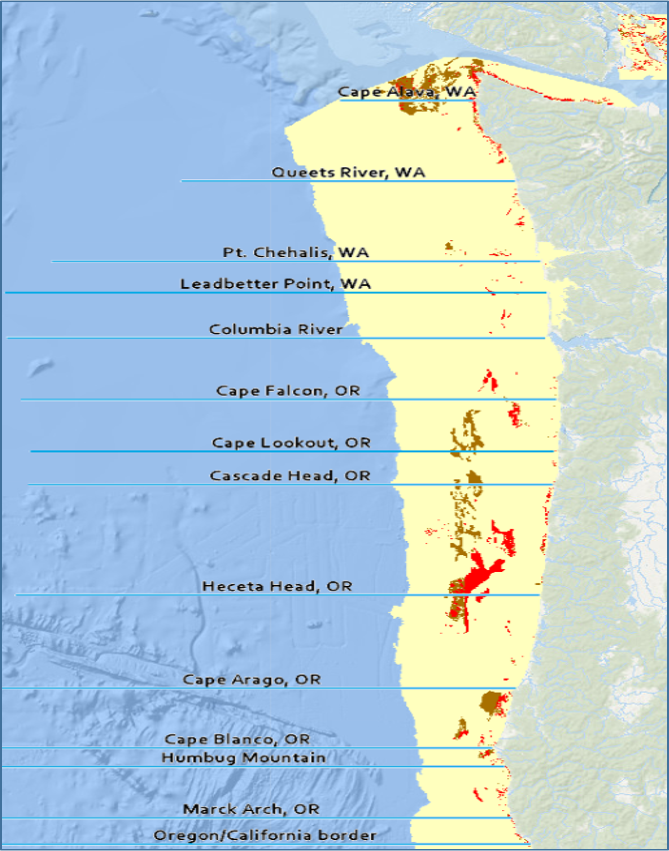
\includegraphics[width=1\textwidth,height=1\textheight]{C:/Users/Jason.Cope/Documents/Github/Vermilion rockfish OR WA assessment 2021/OR/write_up/figures/stock/Vermilion_Map.png}
\caption{Oregon and Washington coastlines with rocky habitat indicated by brown shaded areas. Circled areas represent areas of primary vermilion rockfish occurence..\label{fig:ORWA-map}}
\end{figure}

\tagmcend\tagstructend

\tagstructbegin{tag=Figure,alttext={Total mortality from the southern Oregon and northern Washington recreational fisheries. These represent ninty and ninty-seven percent of the total vermilion removals in each state, respectively..}}\tagmcbegin{tag=Figure}

\begin{figure}
\centering
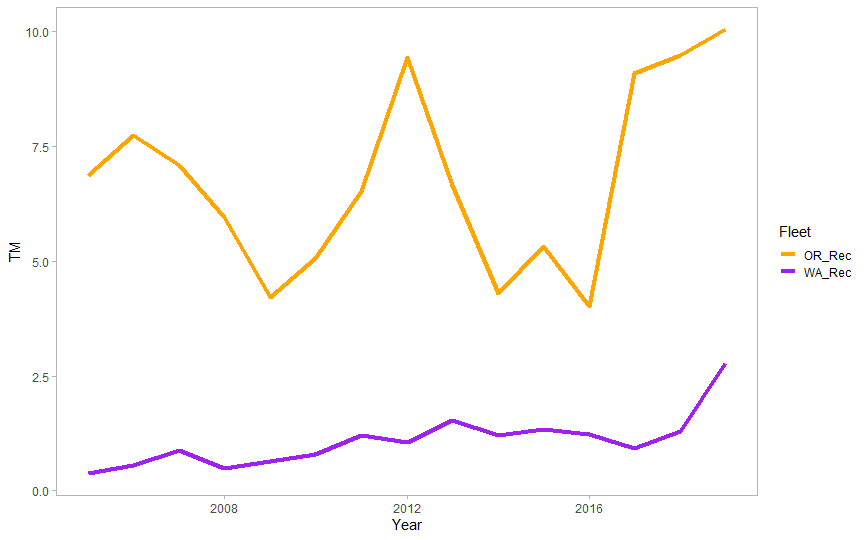
\includegraphics[width=1\textwidth,height=1\textheight]{C:/Users/Jason.Cope/Documents/Github/Vermilion rockfish OR WA assessment 2021/OR/write_up/figures/stock/TM_Vermilion_ORWA.png}
\caption{Total mortality from the southern Oregon and northern Washington recreational fisheries. These represent ninty and ninty-seven percent of the total vermilion removals in each state, respectively..\label{fig:tm-plot}}
\end{figure}

\tagmcend\tagstructend

\tagstructbegin{tag=Figure,alttext={Summary of data sources used in the base model.}}\tagmcbegin{tag=Figure}

\begin{figure}
\centering
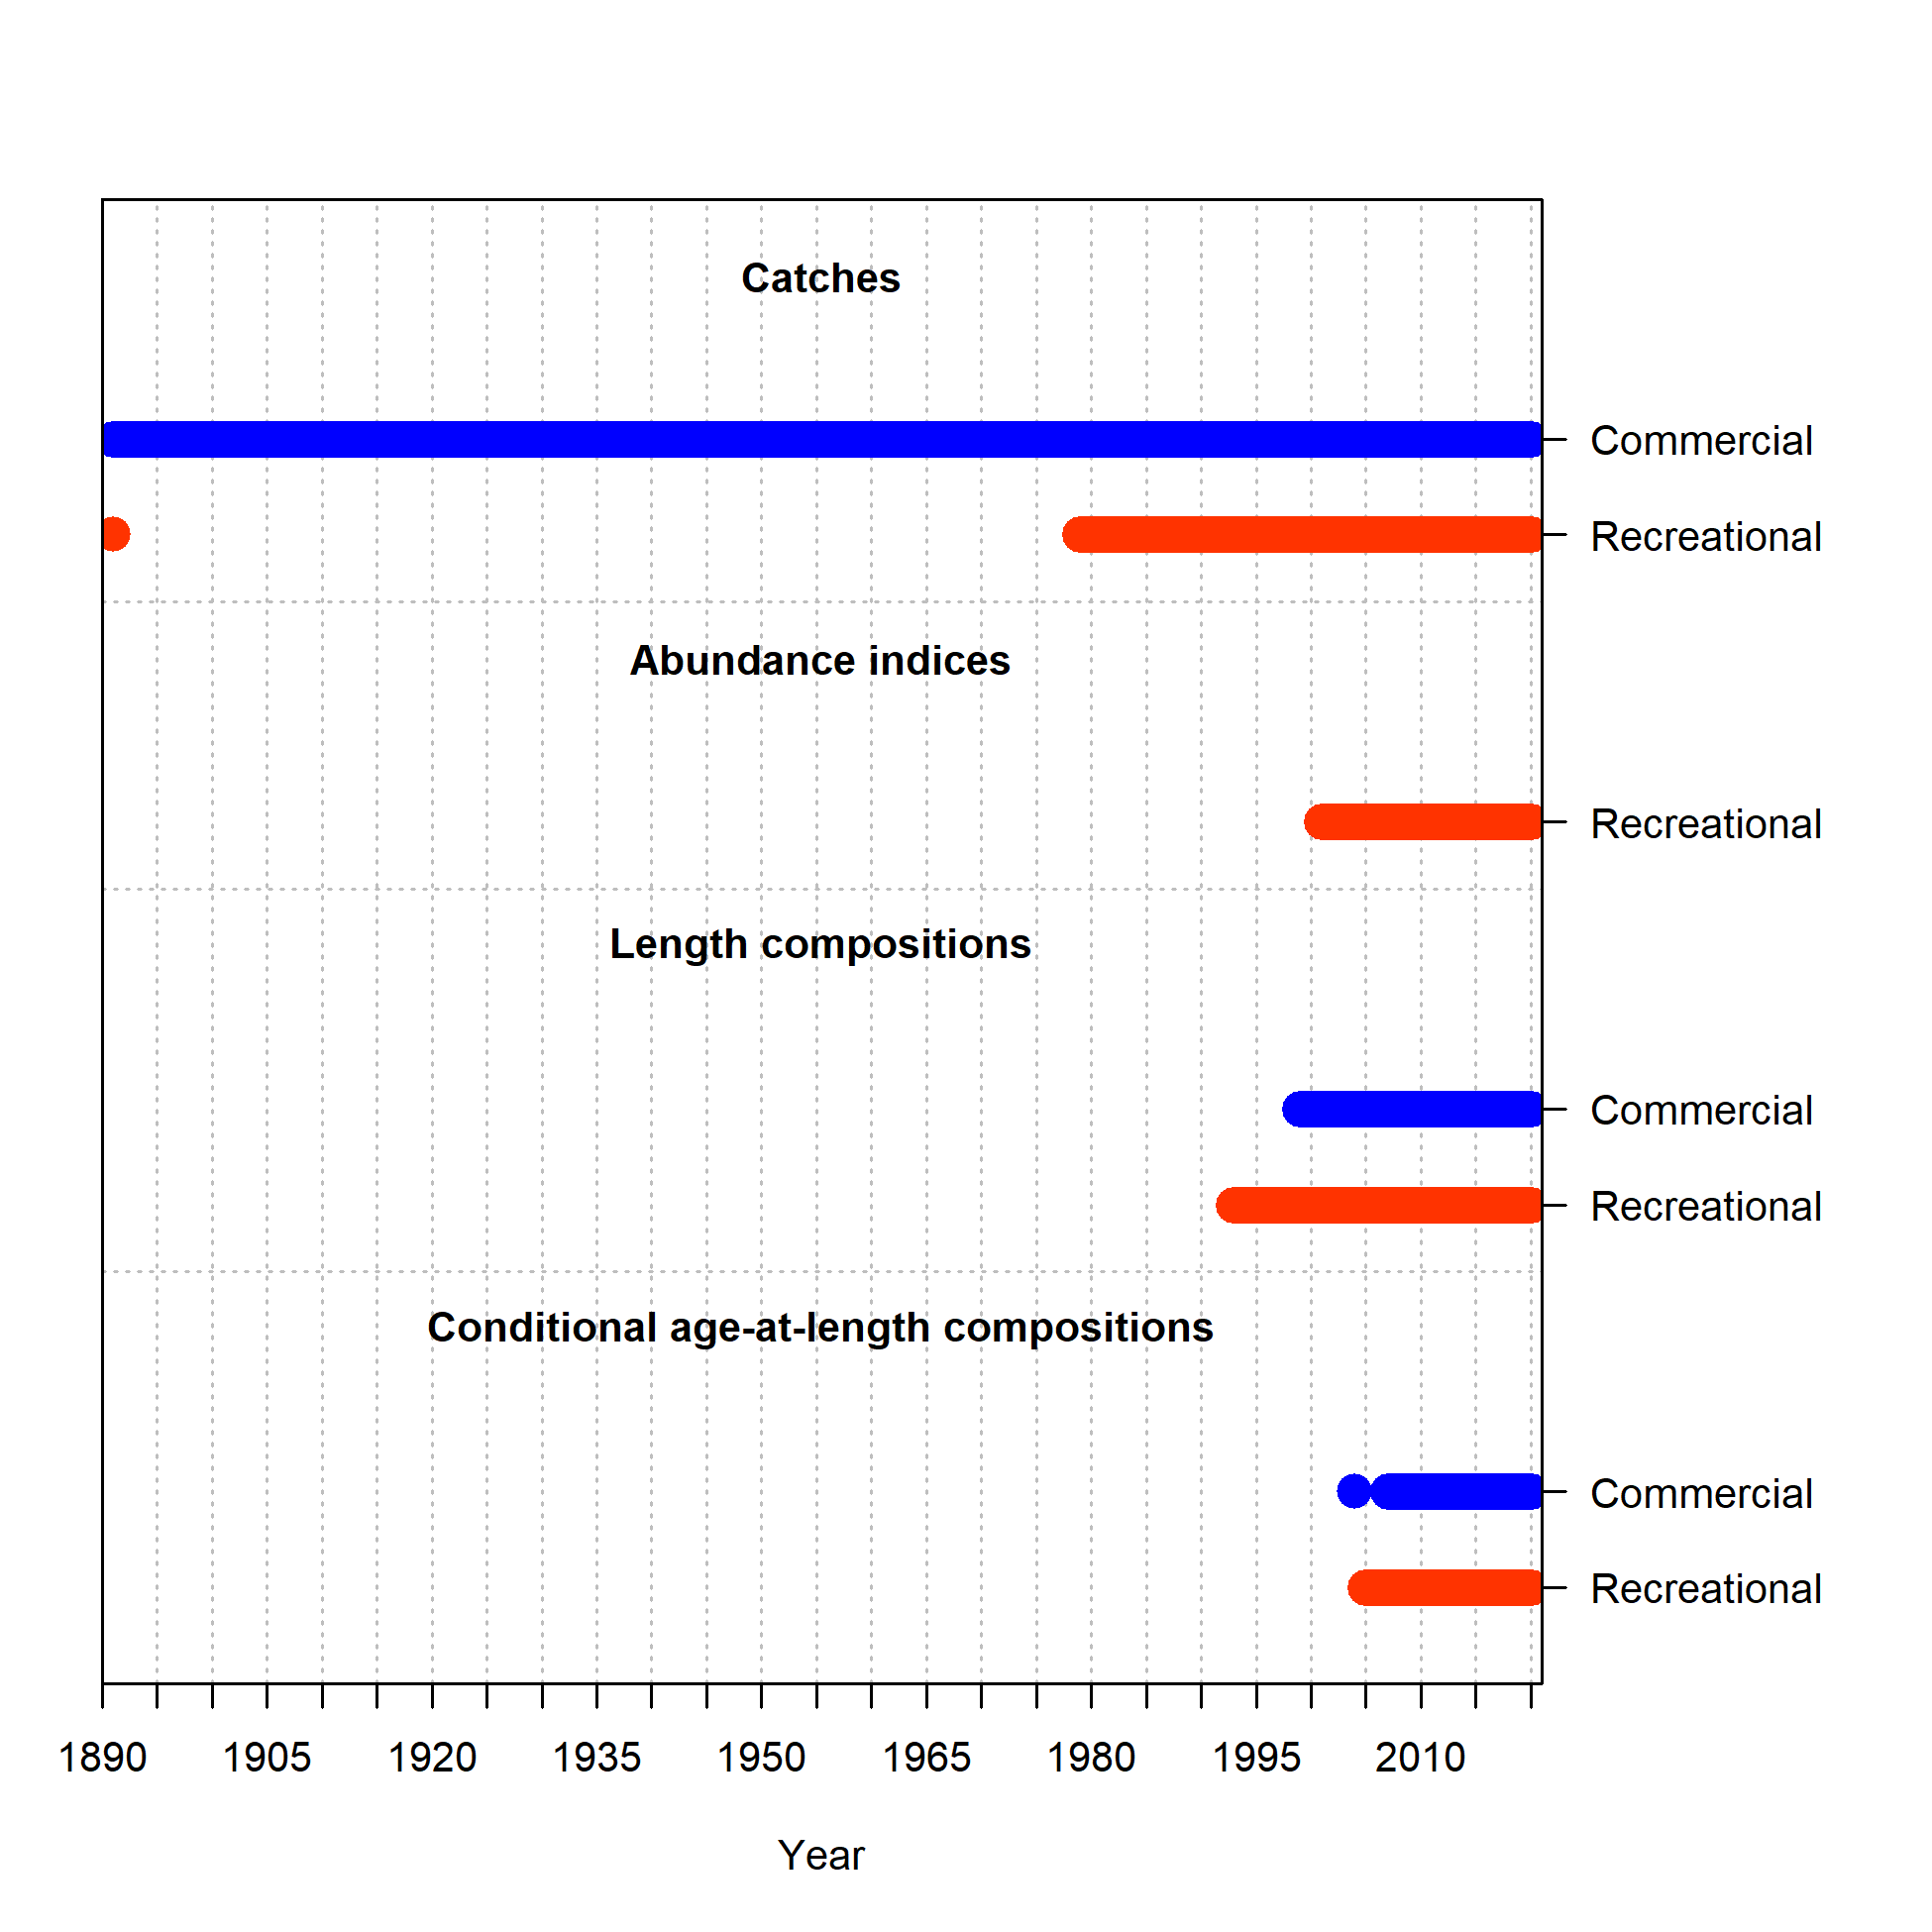
\includegraphics[width=1\textwidth,height=1\textheight]{C:/Users/Jason.Cope/Documents/Github/Vermilion rockfish OR WA assessment 2021/OR/write_up/models/Reference model/plots/data_plot.png}
\caption{Summary of data sources used in the base model.\label{fig:data-plot}}
\end{figure}

\tagmcend\tagstructend

\tagstructbegin{tag=Figure,alttext={Observed length-at-age by data source and sex. Lines indicate fits to the von Bertalanffy growth equation, with parameter estimates provided in the bottom right corner of the figure.}}\tagmcbegin{tag=Figure}

\begin{figure}
\centering
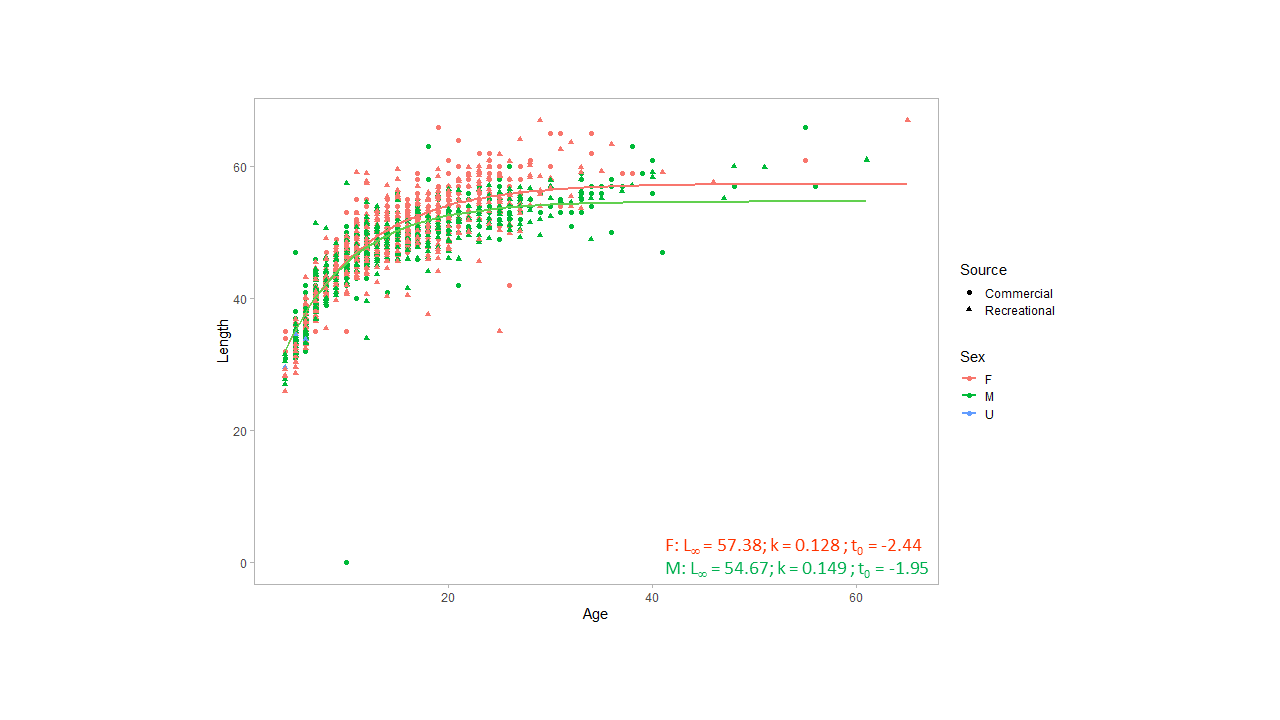
\includegraphics[width=1\textwidth,height=1\textheight]{C:/Users/Jason.Cope/Documents/Github/Vermilion rockfish OR WA assessment 2021/OR/write_up/figures/biology_plots/AG_plot_lines_parameters.png}
\caption{Observed length-at-age by data source and sex. Lines indicate fits to the von Bertalanffy growth equation, with parameter estimates provided in the bottom right corner of the figure.\label{fig:len-age-data}}
\end{figure}

\tagmcend\tagstructend

\tagstructbegin{tag=Figure,alttext={Length at age in the beginning of the year in the ending year of the model.}}\tagmcbegin{tag=Figure}

\begin{figure}
\centering
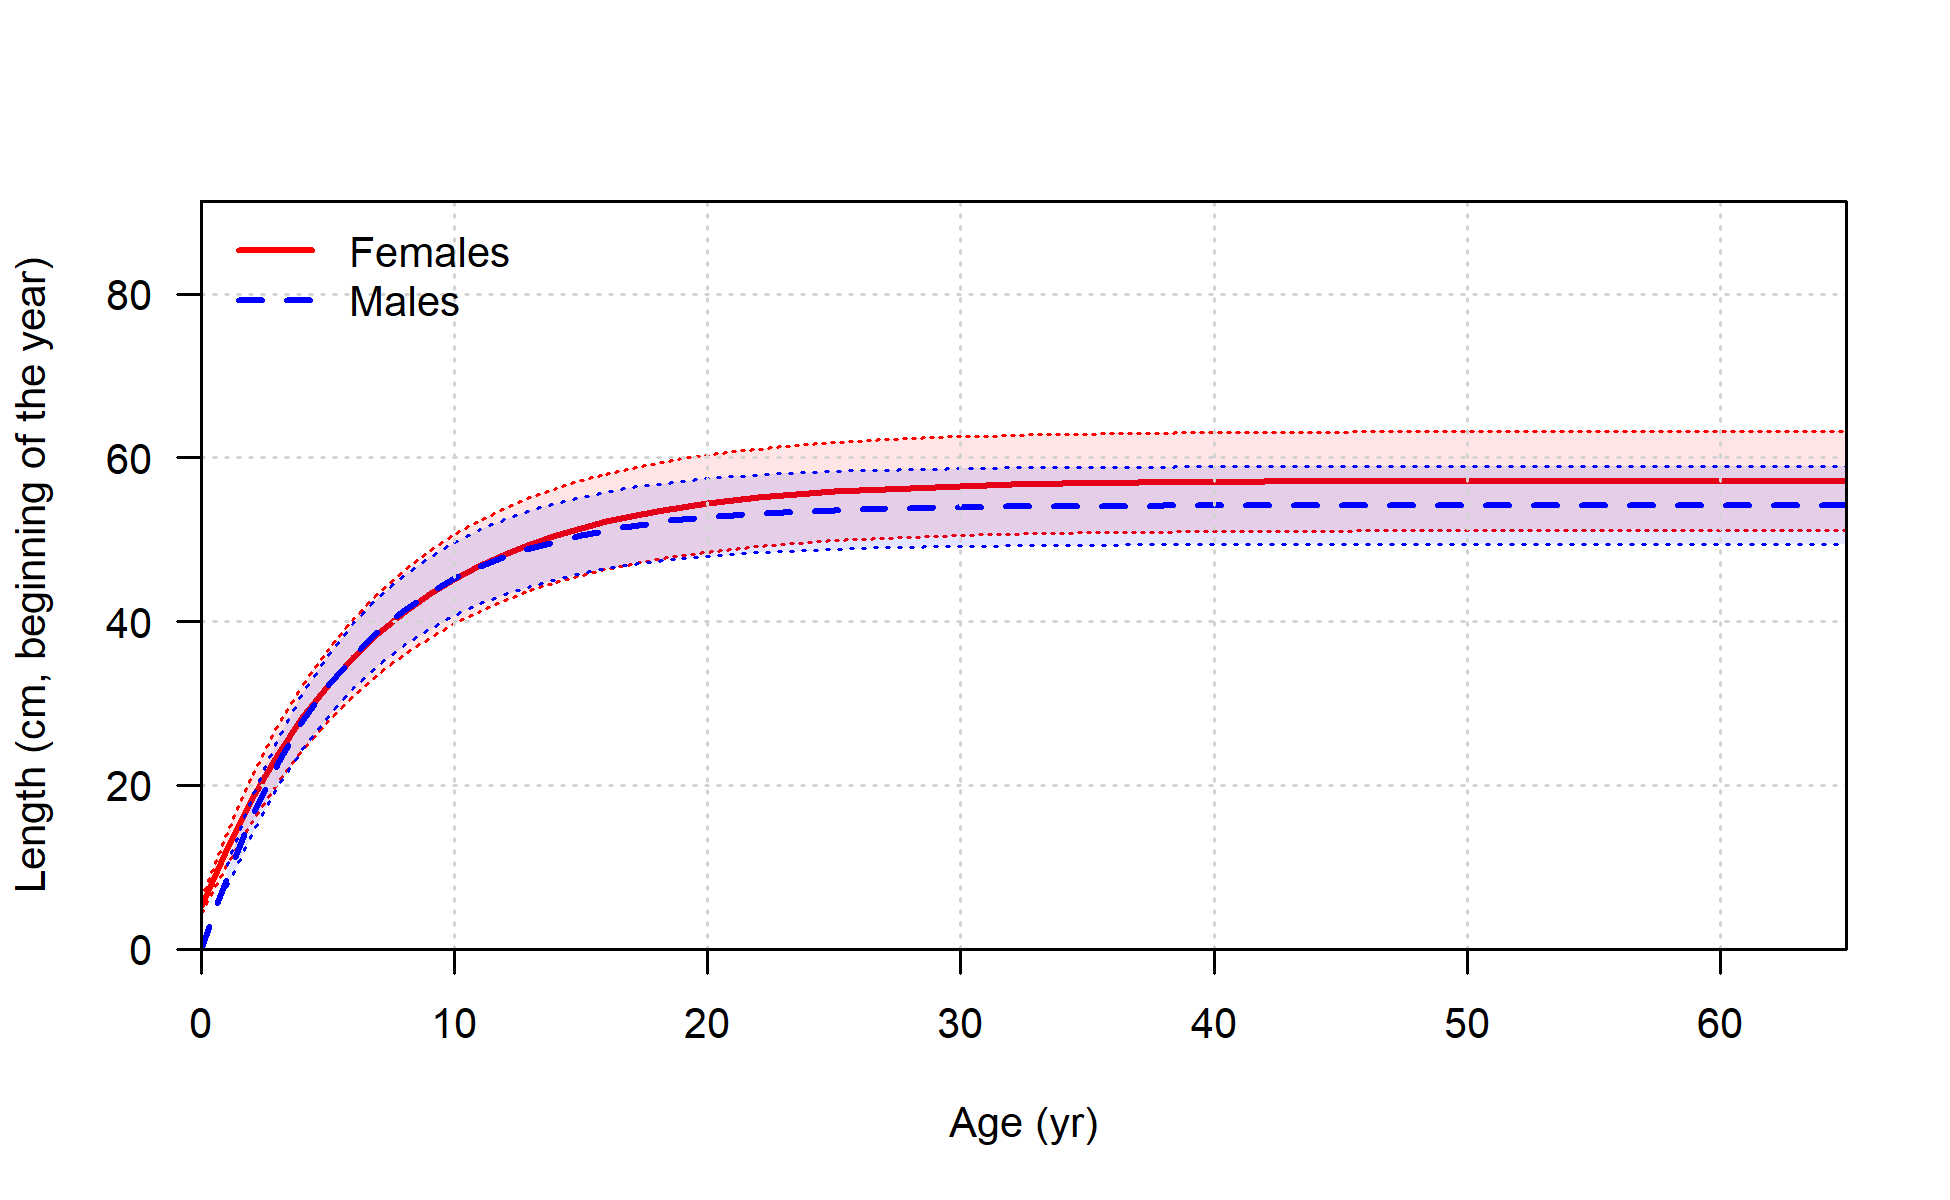
\includegraphics[width=1\textwidth,height=1\textheight]{C:/Users/Jason.Cope/Documents/Github/Vermilion rockfish OR WA assessment 2021/OR/write_up/models/Reference model/plots/bio1_sizeatage.png}
\caption{Length at age in the beginning of the year in the ending year of the model.\label{fig:len-age-ss}}
\end{figure}

\tagmcend\tagstructend

\tagstructbegin{tag=Figure,alttext={Agein error matrix (age by standard deviation) values by source. The commercial and recreational matrices are based on inter-reader comparisons.}}\tagmcbegin{tag=Figure}

\begin{figure}
\centering
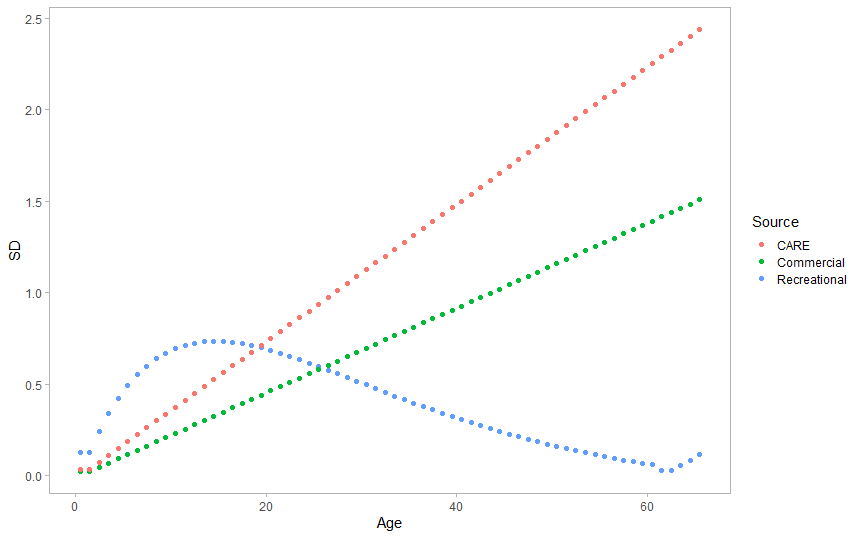
\includegraphics[width=1\textwidth,height=1\textheight]{C:/Users/Jason.Cope/Documents/Github/Vermilion rockfish OR WA assessment 2021/OR/write_up/figures/biology_plots/Age_error_plot.png}
\caption{Agein error matrix (age by standard deviation) values by source. The commercial and recreational matrices are based on inter-reader comparisons.\label{fig:age-error}}
\end{figure}

\tagmcend\tagstructend

\tagstructbegin{tag=Figure,alttext={Maturity as a function of  length.}}\tagmcbegin{tag=Figure}

\begin{figure}
\centering
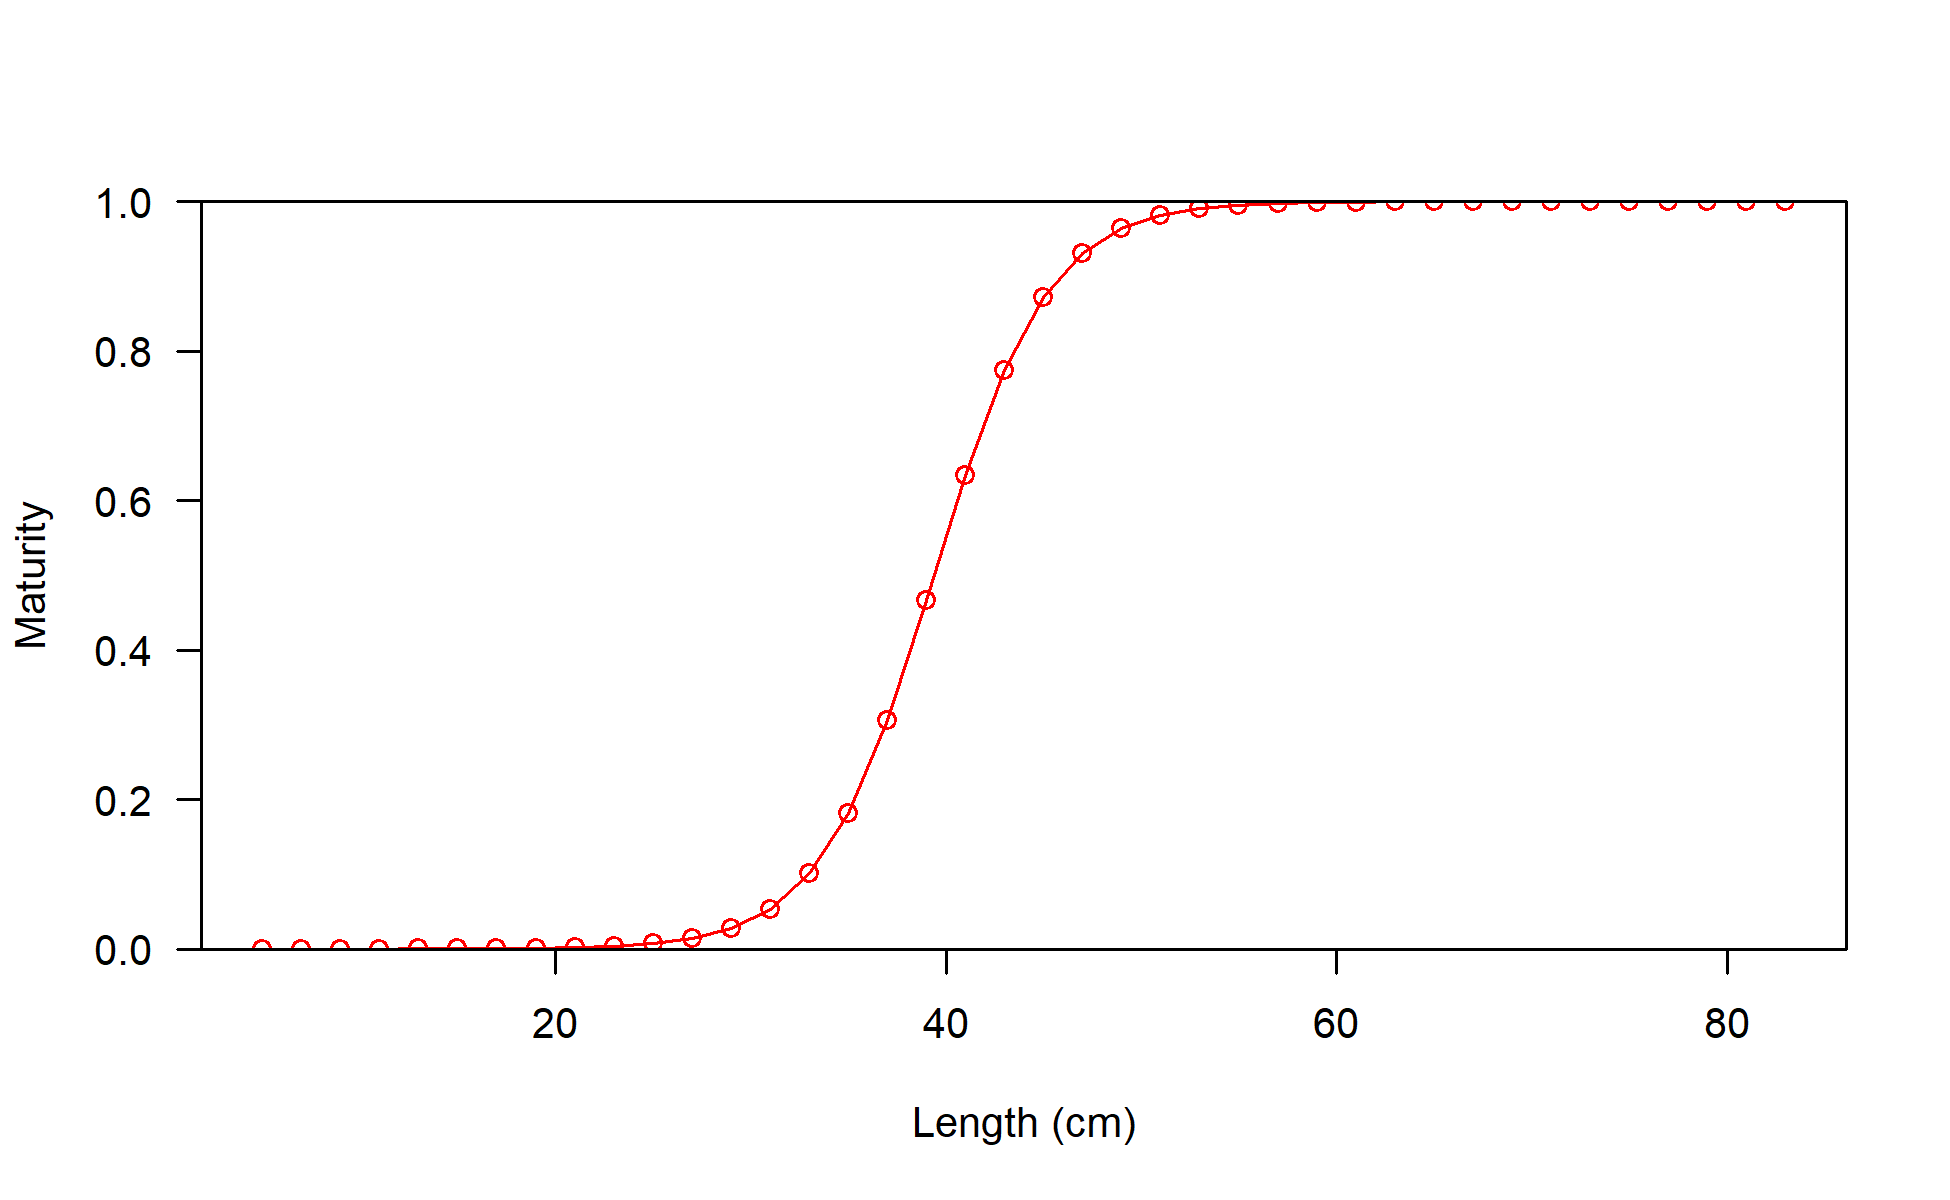
\includegraphics[width=1\textwidth,height=1\textheight]{C:/Users/Jason.Cope/Documents/Github/Vermilion rockfish OR WA assessment 2021/OR/write_up/models/Reference model/plots/bio6_maturity.png}
\caption{Maturity as a function of length.\label{fig:maturity}}
\end{figure}

\tagmcend\tagstructend

\tagstructbegin{tag=Figure,alttext={Fecundity as a function of length.}}\tagmcbegin{tag=Figure}

\begin{figure}
\centering
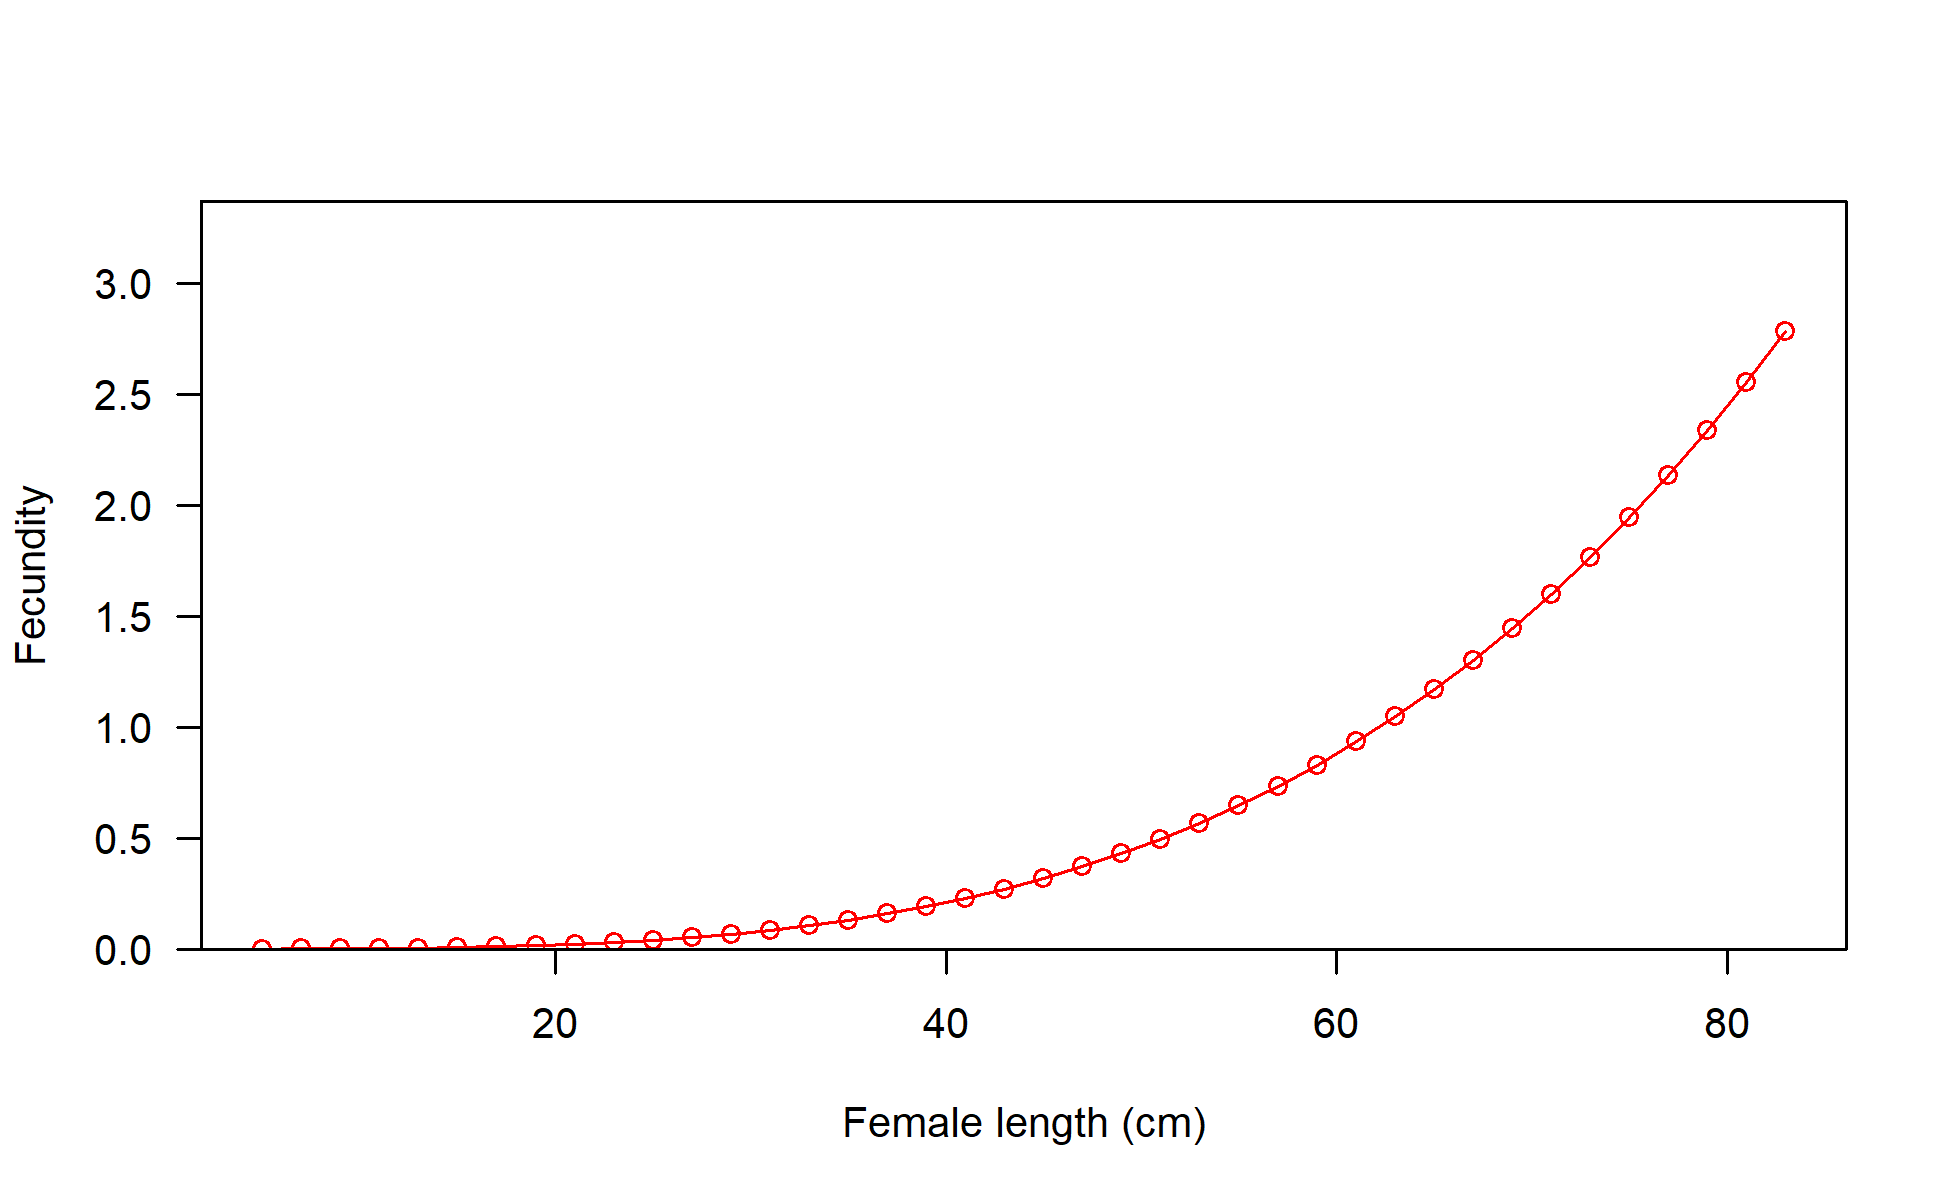
\includegraphics[width=1\textwidth,height=1\textheight]{C:/Users/Jason.Cope/Documents/Github/Vermilion rockfish OR WA assessment 2021/OR/write_up/models/Reference model/plots/bio9_fecundity_len.png}
\caption{Fecundity as a function of length.\label{fig:fecundity}}
\end{figure}

\tagmcend\tagstructend

\tagstructbegin{tag=Figure,alttext={Composite natural mortality distriubtion for $S. hopkinsi$ using four longevity estimators each with a SD = 0.2 presuming a lognomral error distibution.}}\tagmcbegin{tag=Figure}

\begin{figure}
\centering
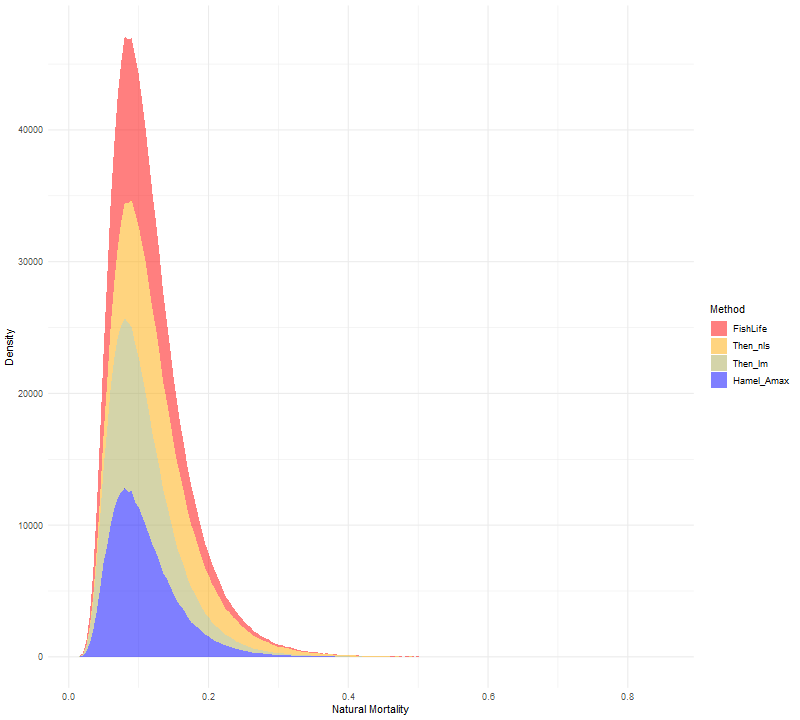
\includegraphics[width=1\textwidth,height=1\textheight]{C:/Users/Jason.Cope/Documents/Github/Vermilion rockfish OR WA assessment 2021/OR/write_up/figures/biology_plots/Mdensityplots_OR_vermilion.png}
\caption{Composite natural mortality distriubtion for {\tagstructbegin{tag=Formula}\tagmcbegin{tag=Formula}\(S. hopkinsi\)\leavevmode\tagmcend\tagstructend} using four longevity estimators each with a SD = 0.2 presuming a lognomral error distibution.\label{fig:M_composite_dists}}
\end{figure}

\tagmcend\tagstructend

\tagstructbegin{tag=Figure,alttext={Length-weight data and fits to commercially-derived sex-specific vermilion samples.}}\tagmcbegin{tag=Figure}

\begin{figure}
\centering
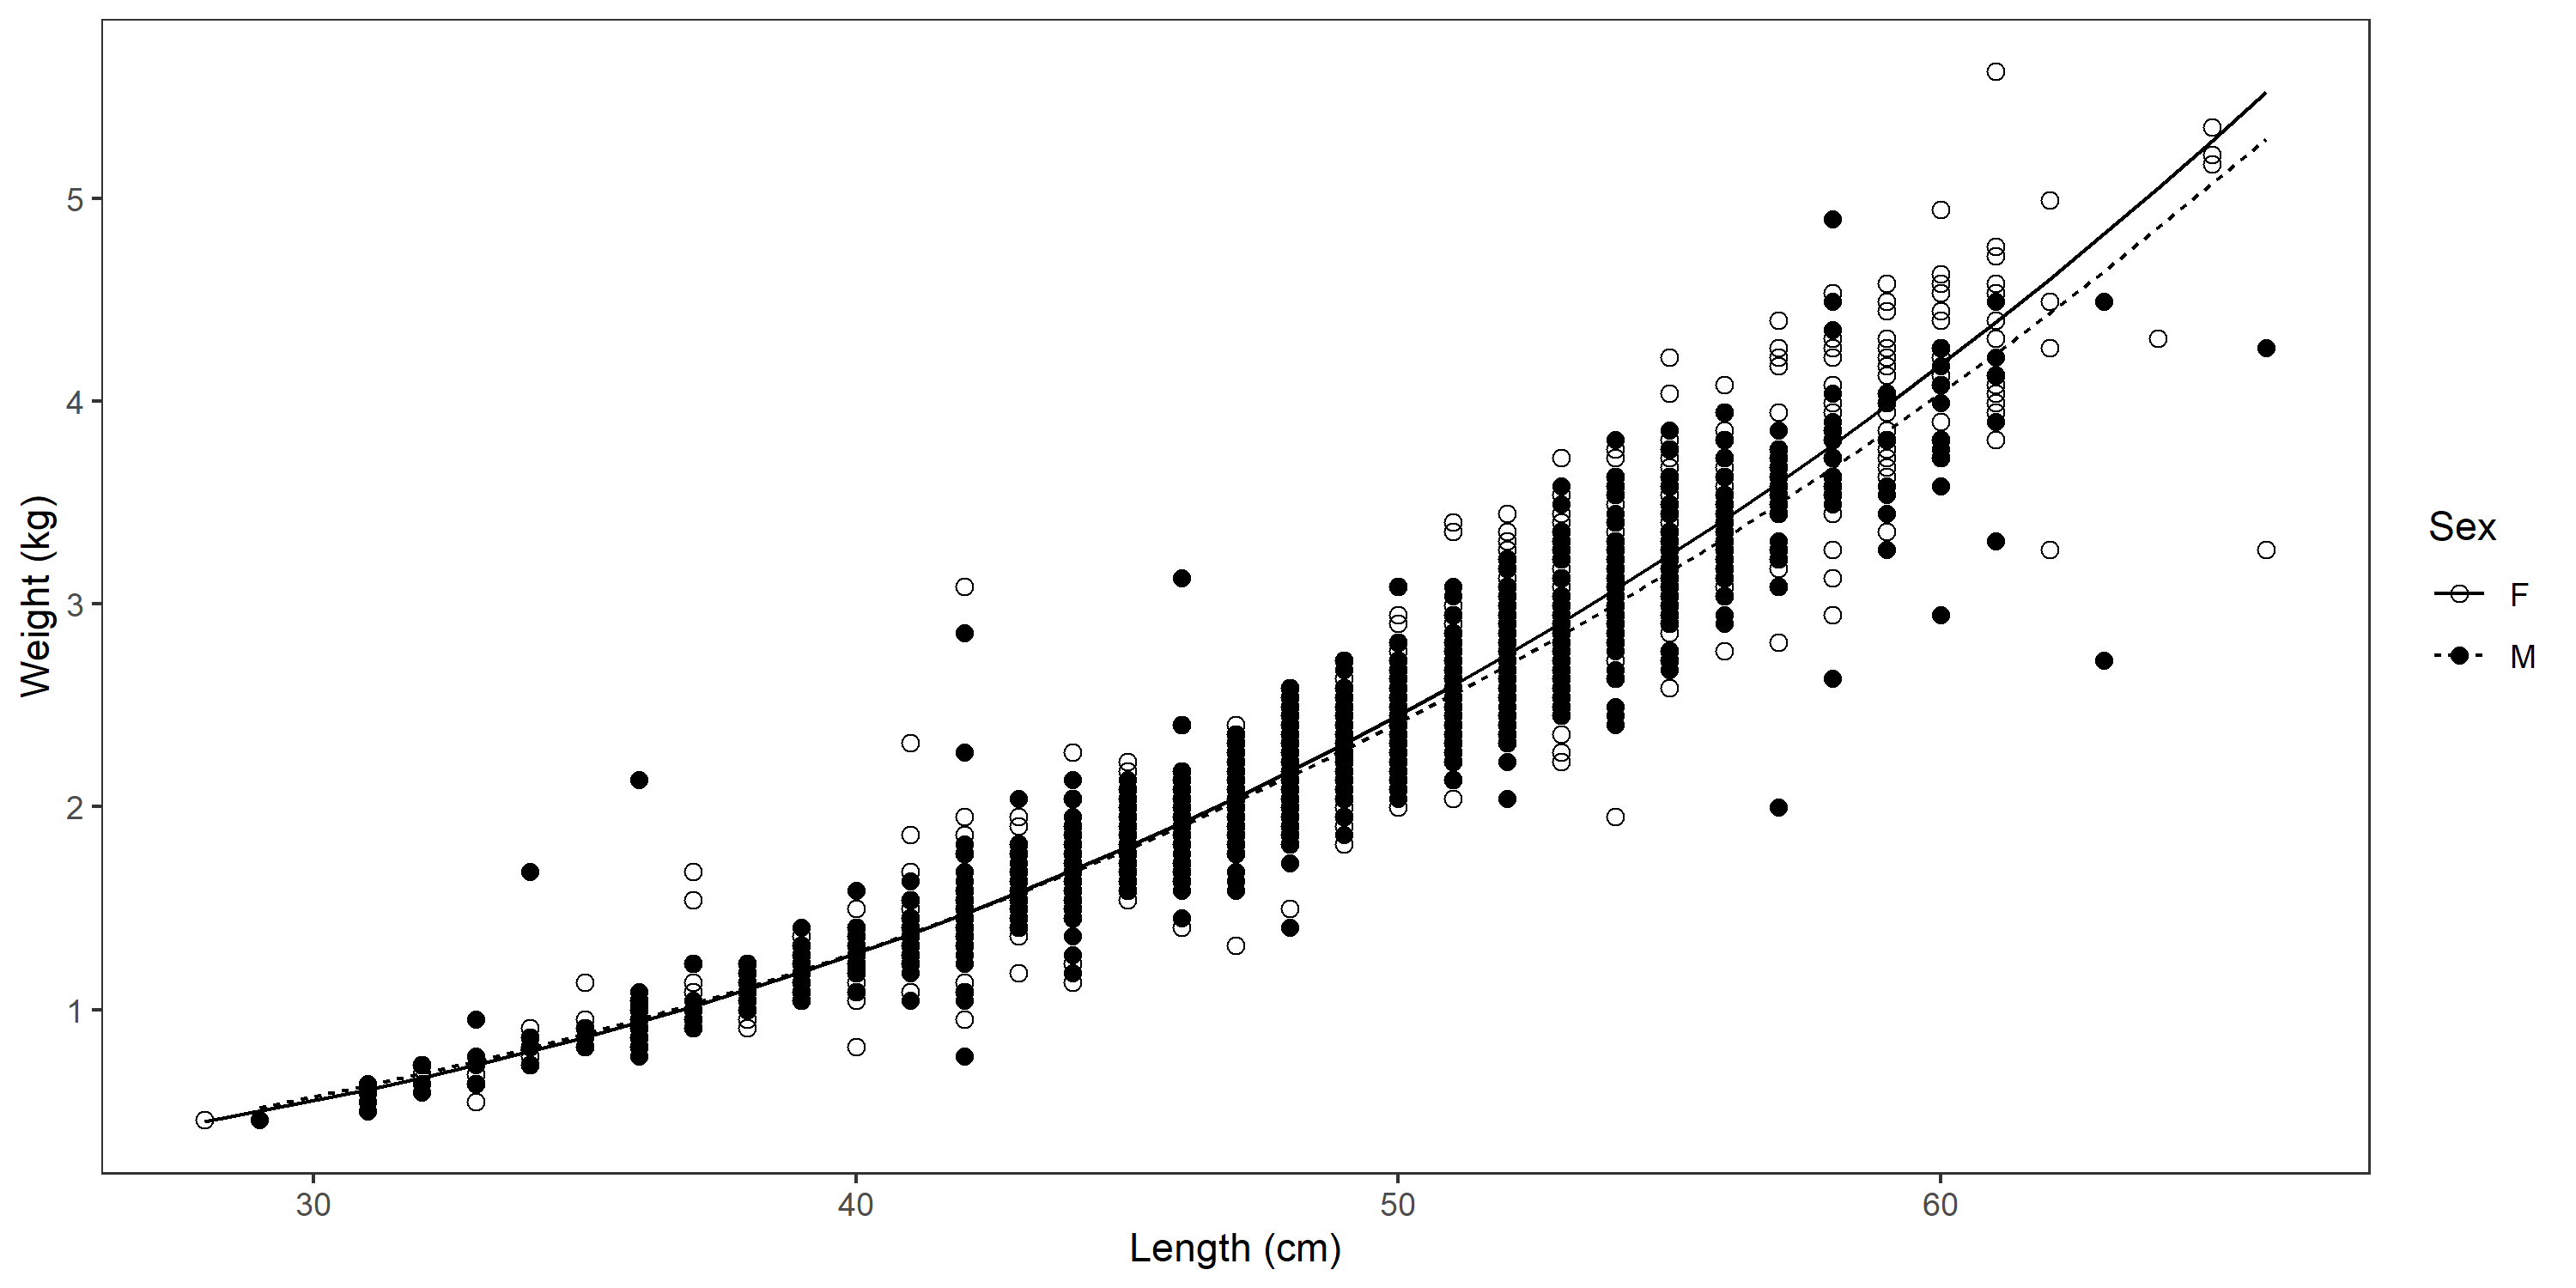
\includegraphics[width=1\textwidth,height=1\textheight]{C:/Users/Jason.Cope/Documents/Github/Vermilion rockfish OR WA assessment 2021/OR/write_up/figures/biology_plots/OR_Vermilion_Sexed Length vs Weight_withpower.png}
\caption{Length-weight data and fits to commercially-derived sex-specific vermilion samples.\label{fig:len-weight-fit}}
\end{figure}

\tagmcend\tagstructend

\tagstructbegin{tag=Figure,alttext={Selectivity at length by fleet.}}\tagmcbegin{tag=Figure}

\begin{figure}
\centering
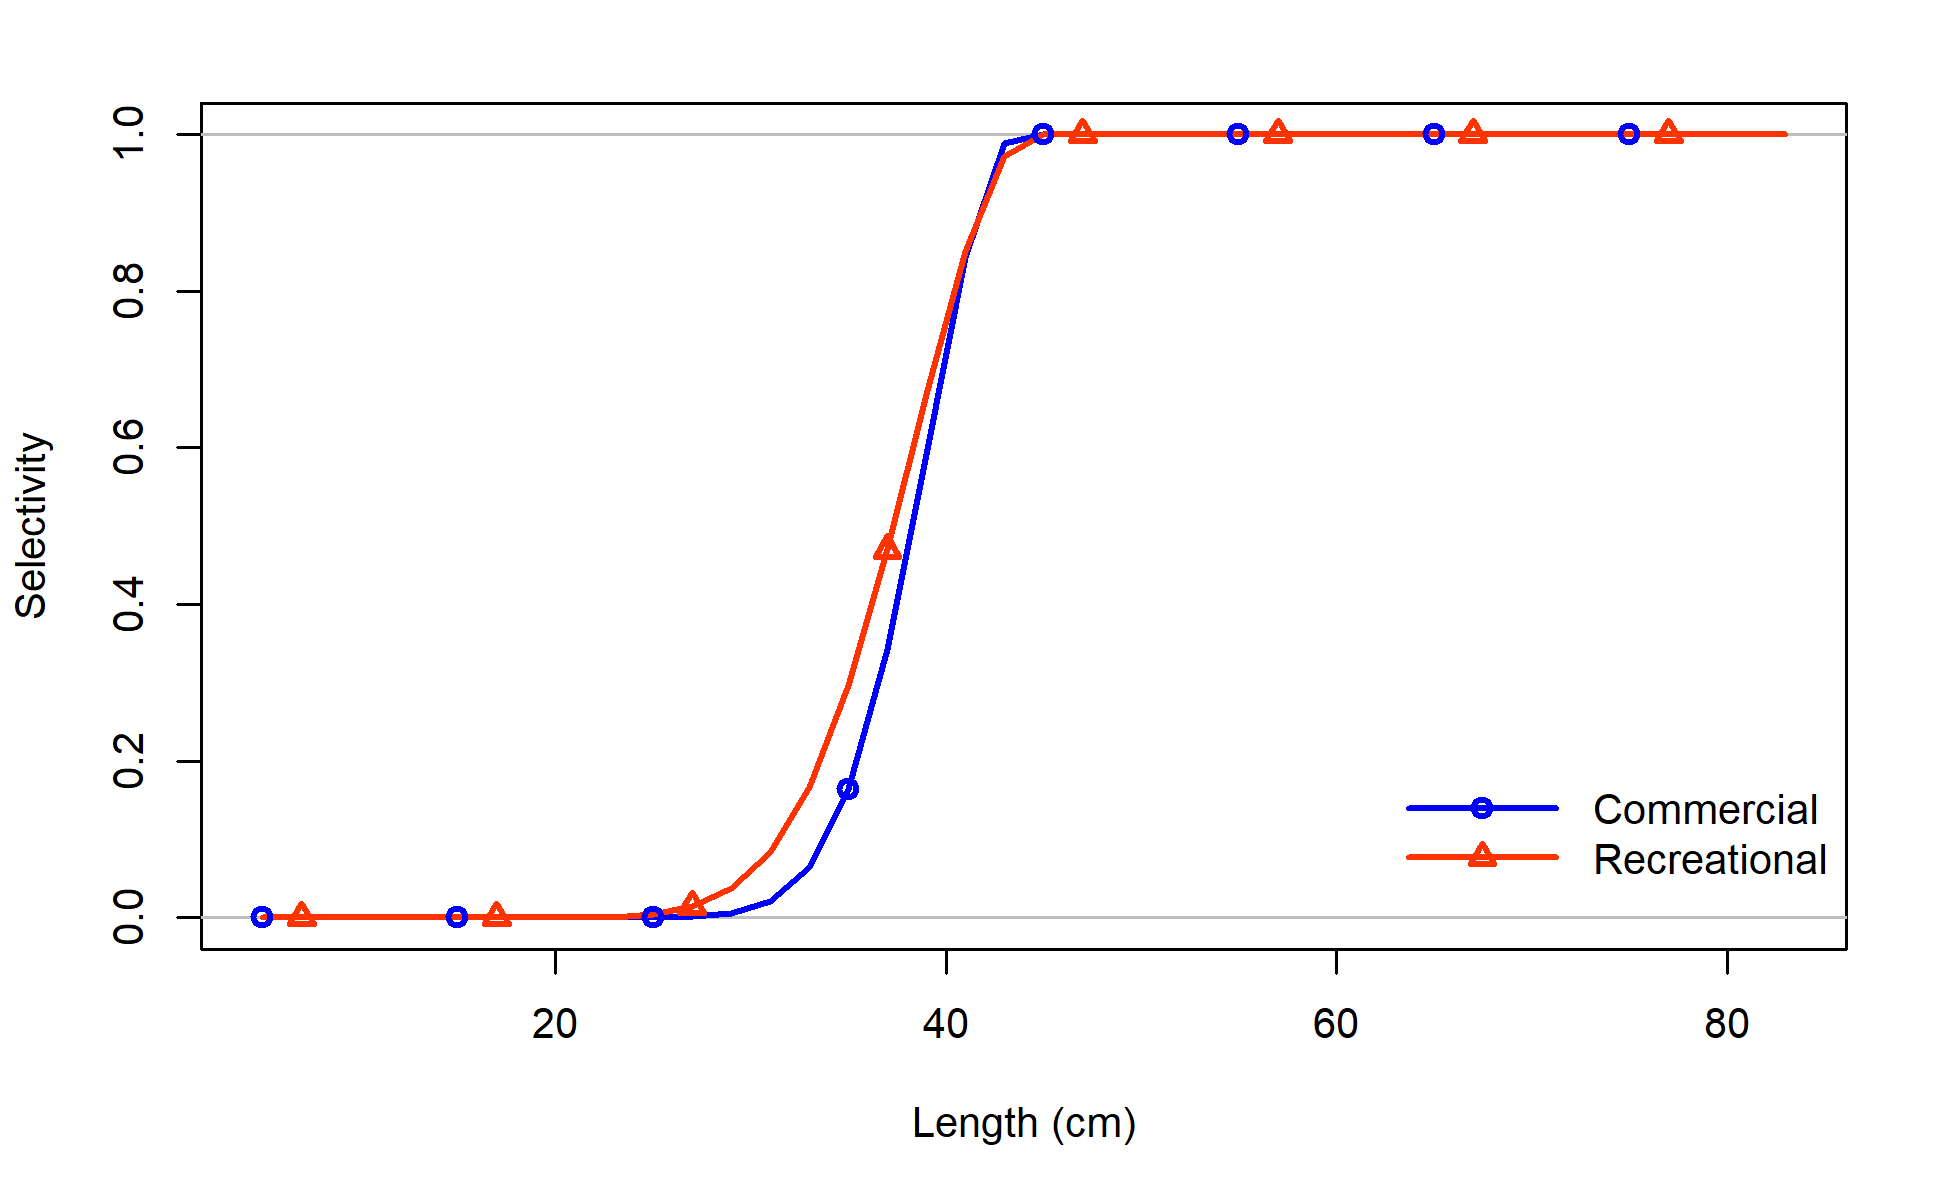
\includegraphics[width=1\textwidth,height=1\textheight]{C:/Users/Jason.Cope/Documents/Github/Vermilion rockfish OR WA assessment 2021/OR/write_up/models/Reference model/plots/sel01_multiple_fleets_length1.png}
\caption{Selectivity at length by fleet.\label{fig:selex}}
\end{figure}

\tagmcend\tagstructend

\tagstructbegin{tag=Figure,alttext={Jitter runs for the squarespot rockfish reference model, with jitter run number on the x-axis and -log likelihood value on the y-axis. Blue dot are models that match the likelihood value of the reference model, while red dots deviate from the reference model. All red dots are above the blue dots, indicating no better fit to the reference model was found.}}\tagmcbegin{tag=Figure}

\begin{figure}
\centering
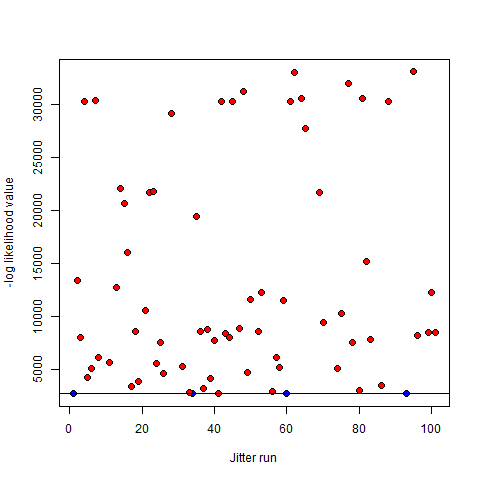
\includegraphics[width=1\textwidth,height=1\textheight]{C:/Users/Jason.Cope/Documents/Github/Vermilion rockfish OR WA assessment 2021/OR/write_up/models/Reference model/Jitter Results/jitterplot_01.png}
\caption{Jitter runs for the squarespot rockfish reference model, with jitter run number on the x-axis and -log likelihood value on the y-axis. Blue dot are models that match the likelihood value of the reference model, while red dots deviate from the reference model. All red dots are above the blue dots, indicating no better fit to the reference model was found.\label{fig:jitter_01}}
\end{figure}

\tagmcend\tagstructend

\tagstructbegin{tag=Figure,alttext={Pearson residuals for the commercial (top panel) and recreational (bottom panel) fleet. Closed bubble are positive residuals (observed > expected) and open bubbles are negative residuals (observed < expected).}}\tagmcbegin{tag=Figure}

\begin{figure}
\centering
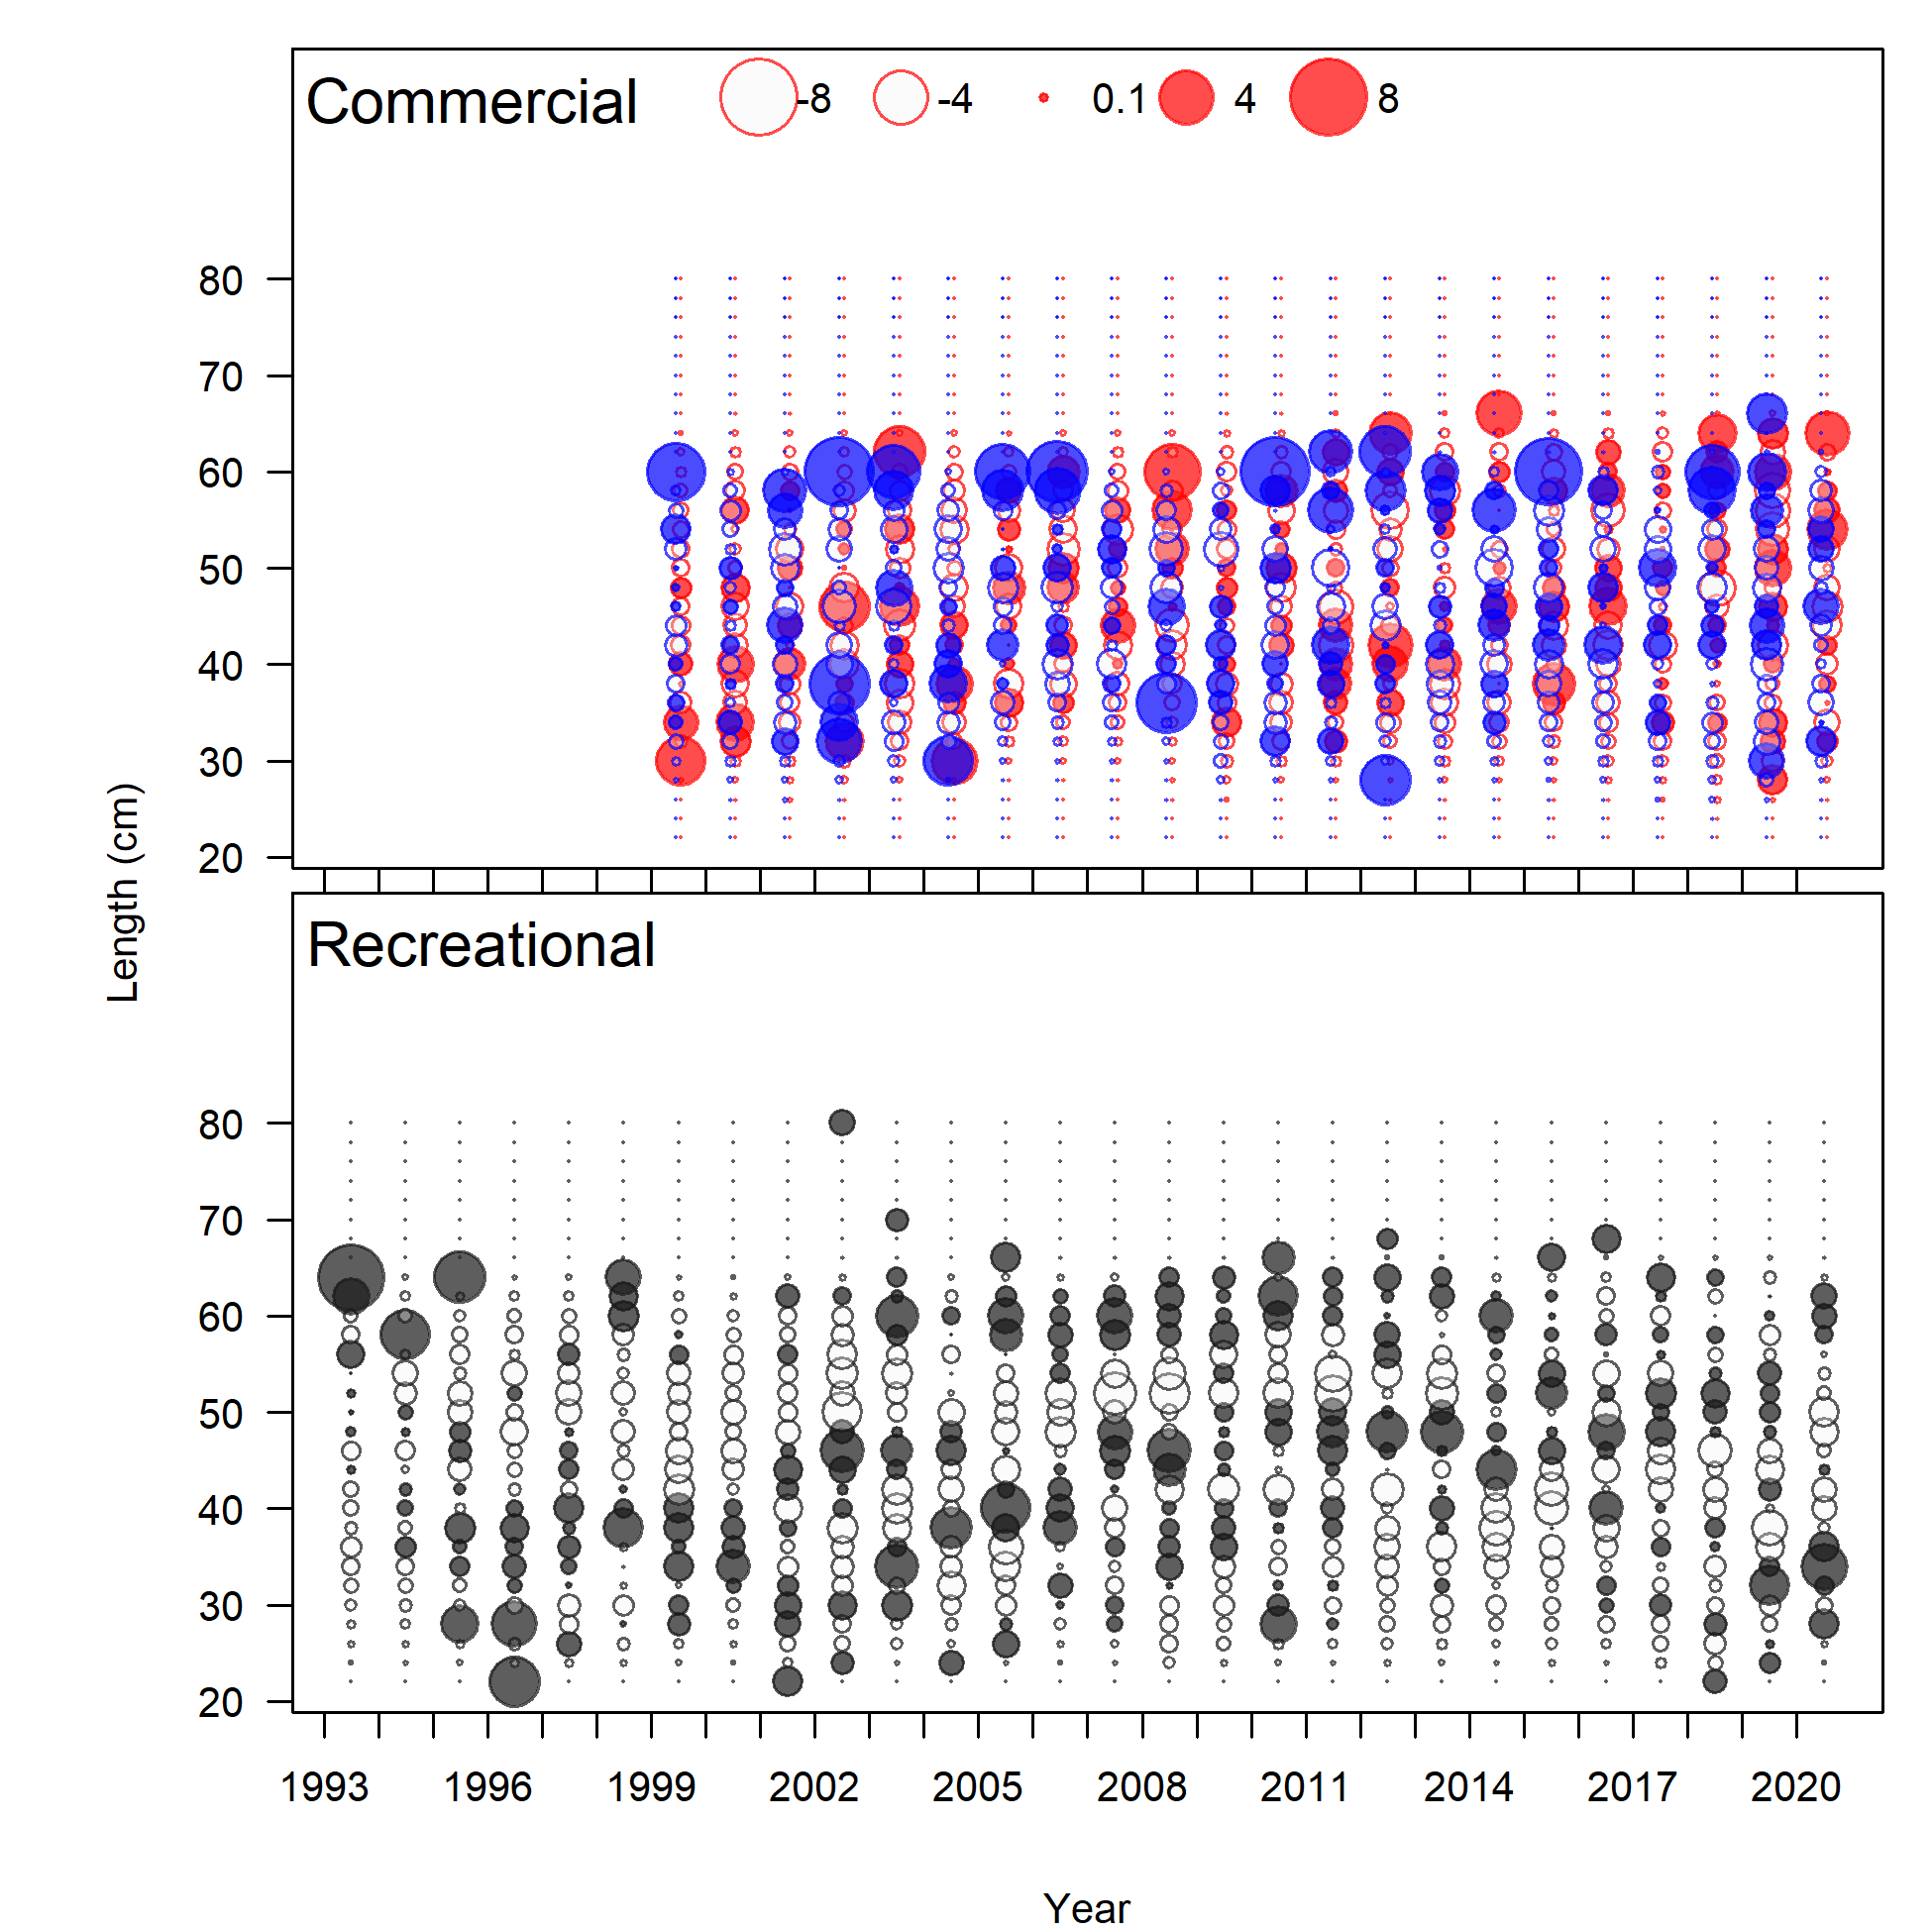
\includegraphics[width=1\textwidth,height=1\textheight]{C:/Users/Jason.Cope/Documents/Github/Vermilion rockfish OR WA assessment 2021/OR/write_up/models/Reference model/plots/comp_lenfit__multi-fleet_comparison.png}
\caption{Pearson residuals for the commercial (top panel) and recreational (bottom panel) fleet. Closed bubble are positive residuals (observed \textgreater{} expected) and open bubbles are negative residuals (observed \textless{} expected).\label{fig:com-rec-pearson}}
\end{figure}

\tagmcend\tagstructend

\tagstructbegin{tag=Figure,alttext={Mean length index from the commercial fishery with 95 percent confidence intervals based on sample sizes and data weighting.}}\tagmcbegin{tag=Figure}

\begin{figure}
\centering
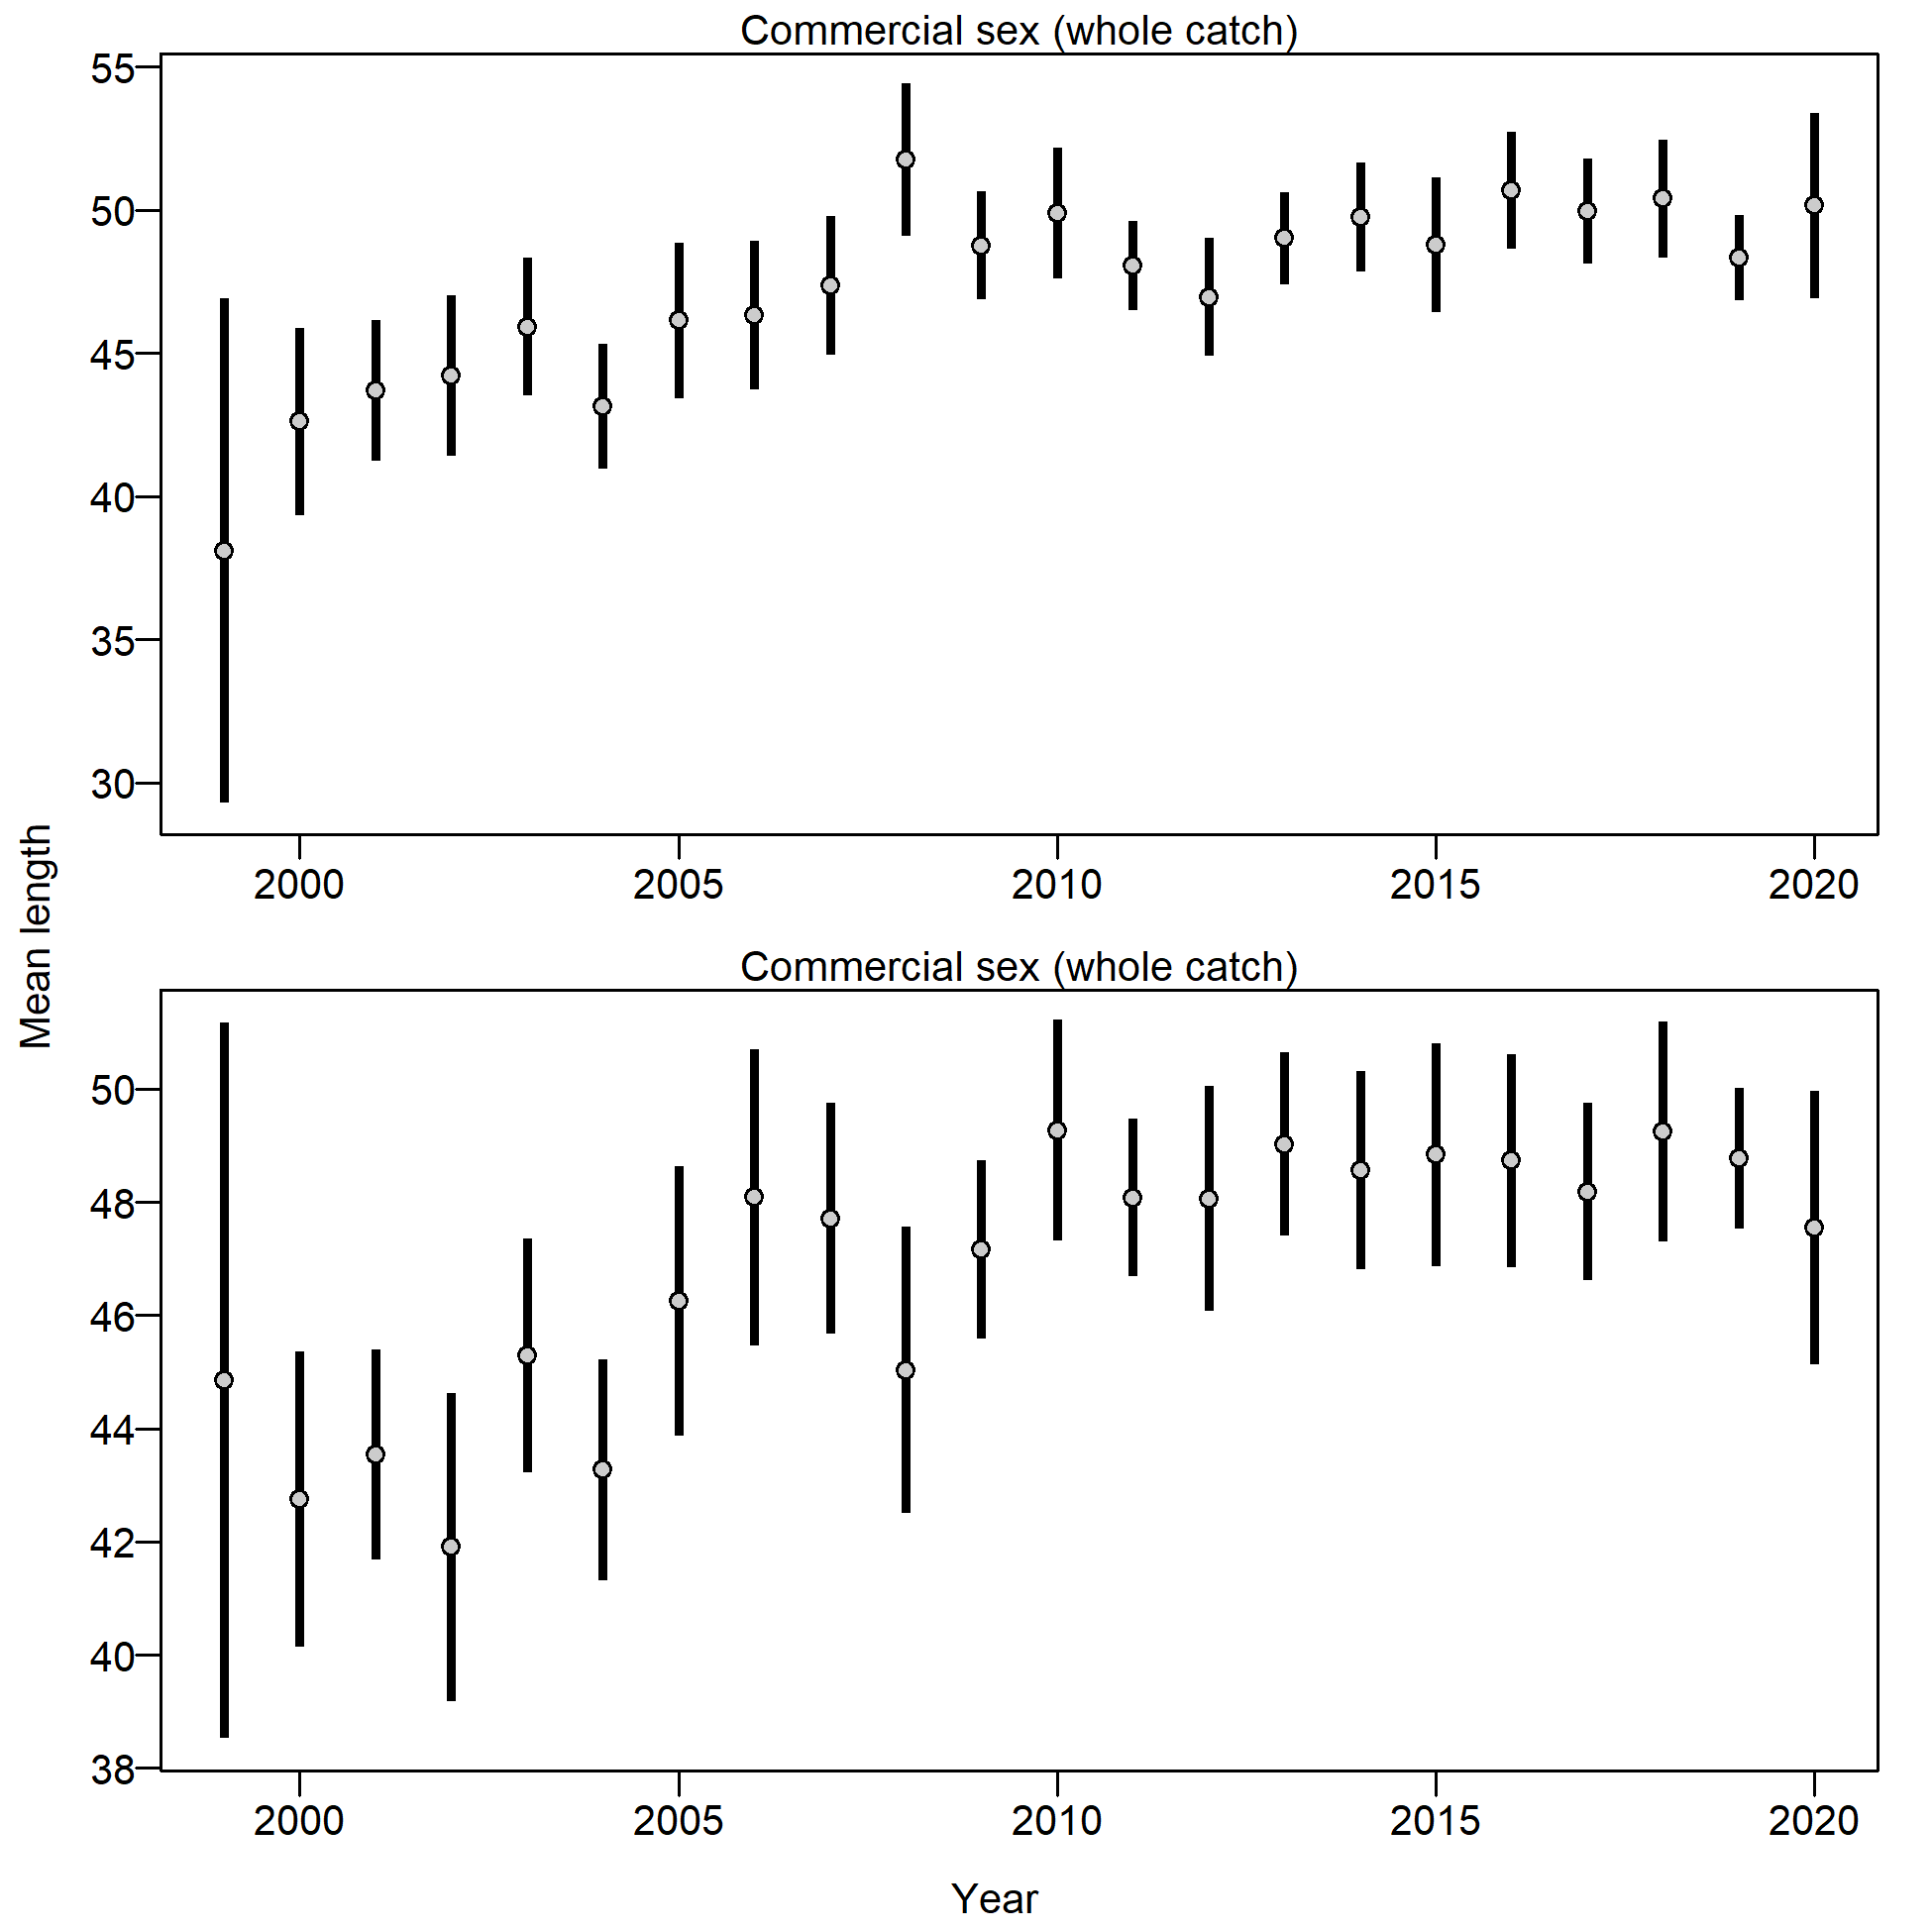
\includegraphics[width=1\textwidth,height=1\textheight]{C:/Users/Jason.Cope/Documents/Github/Vermilion rockfish OR WA assessment 2021/OR/write_up/models/Reference model/plots/comp_lendat_data_weighting_TA1.8_Commercial.png}
\caption{Mean length index from the commercial fishery with 95 percent confidence intervals based on sample sizes and data weighting.\label{fig:com-mean-len-fit}}
\end{figure}

\tagmcend\tagstructend

\tagstructbegin{tag=Figure,alttext={Mean length index from the recreational fishery with 95 percent confidence intervals based on sample sizes and data weighting.}}\tagmcbegin{tag=Figure}

\begin{figure}
\centering
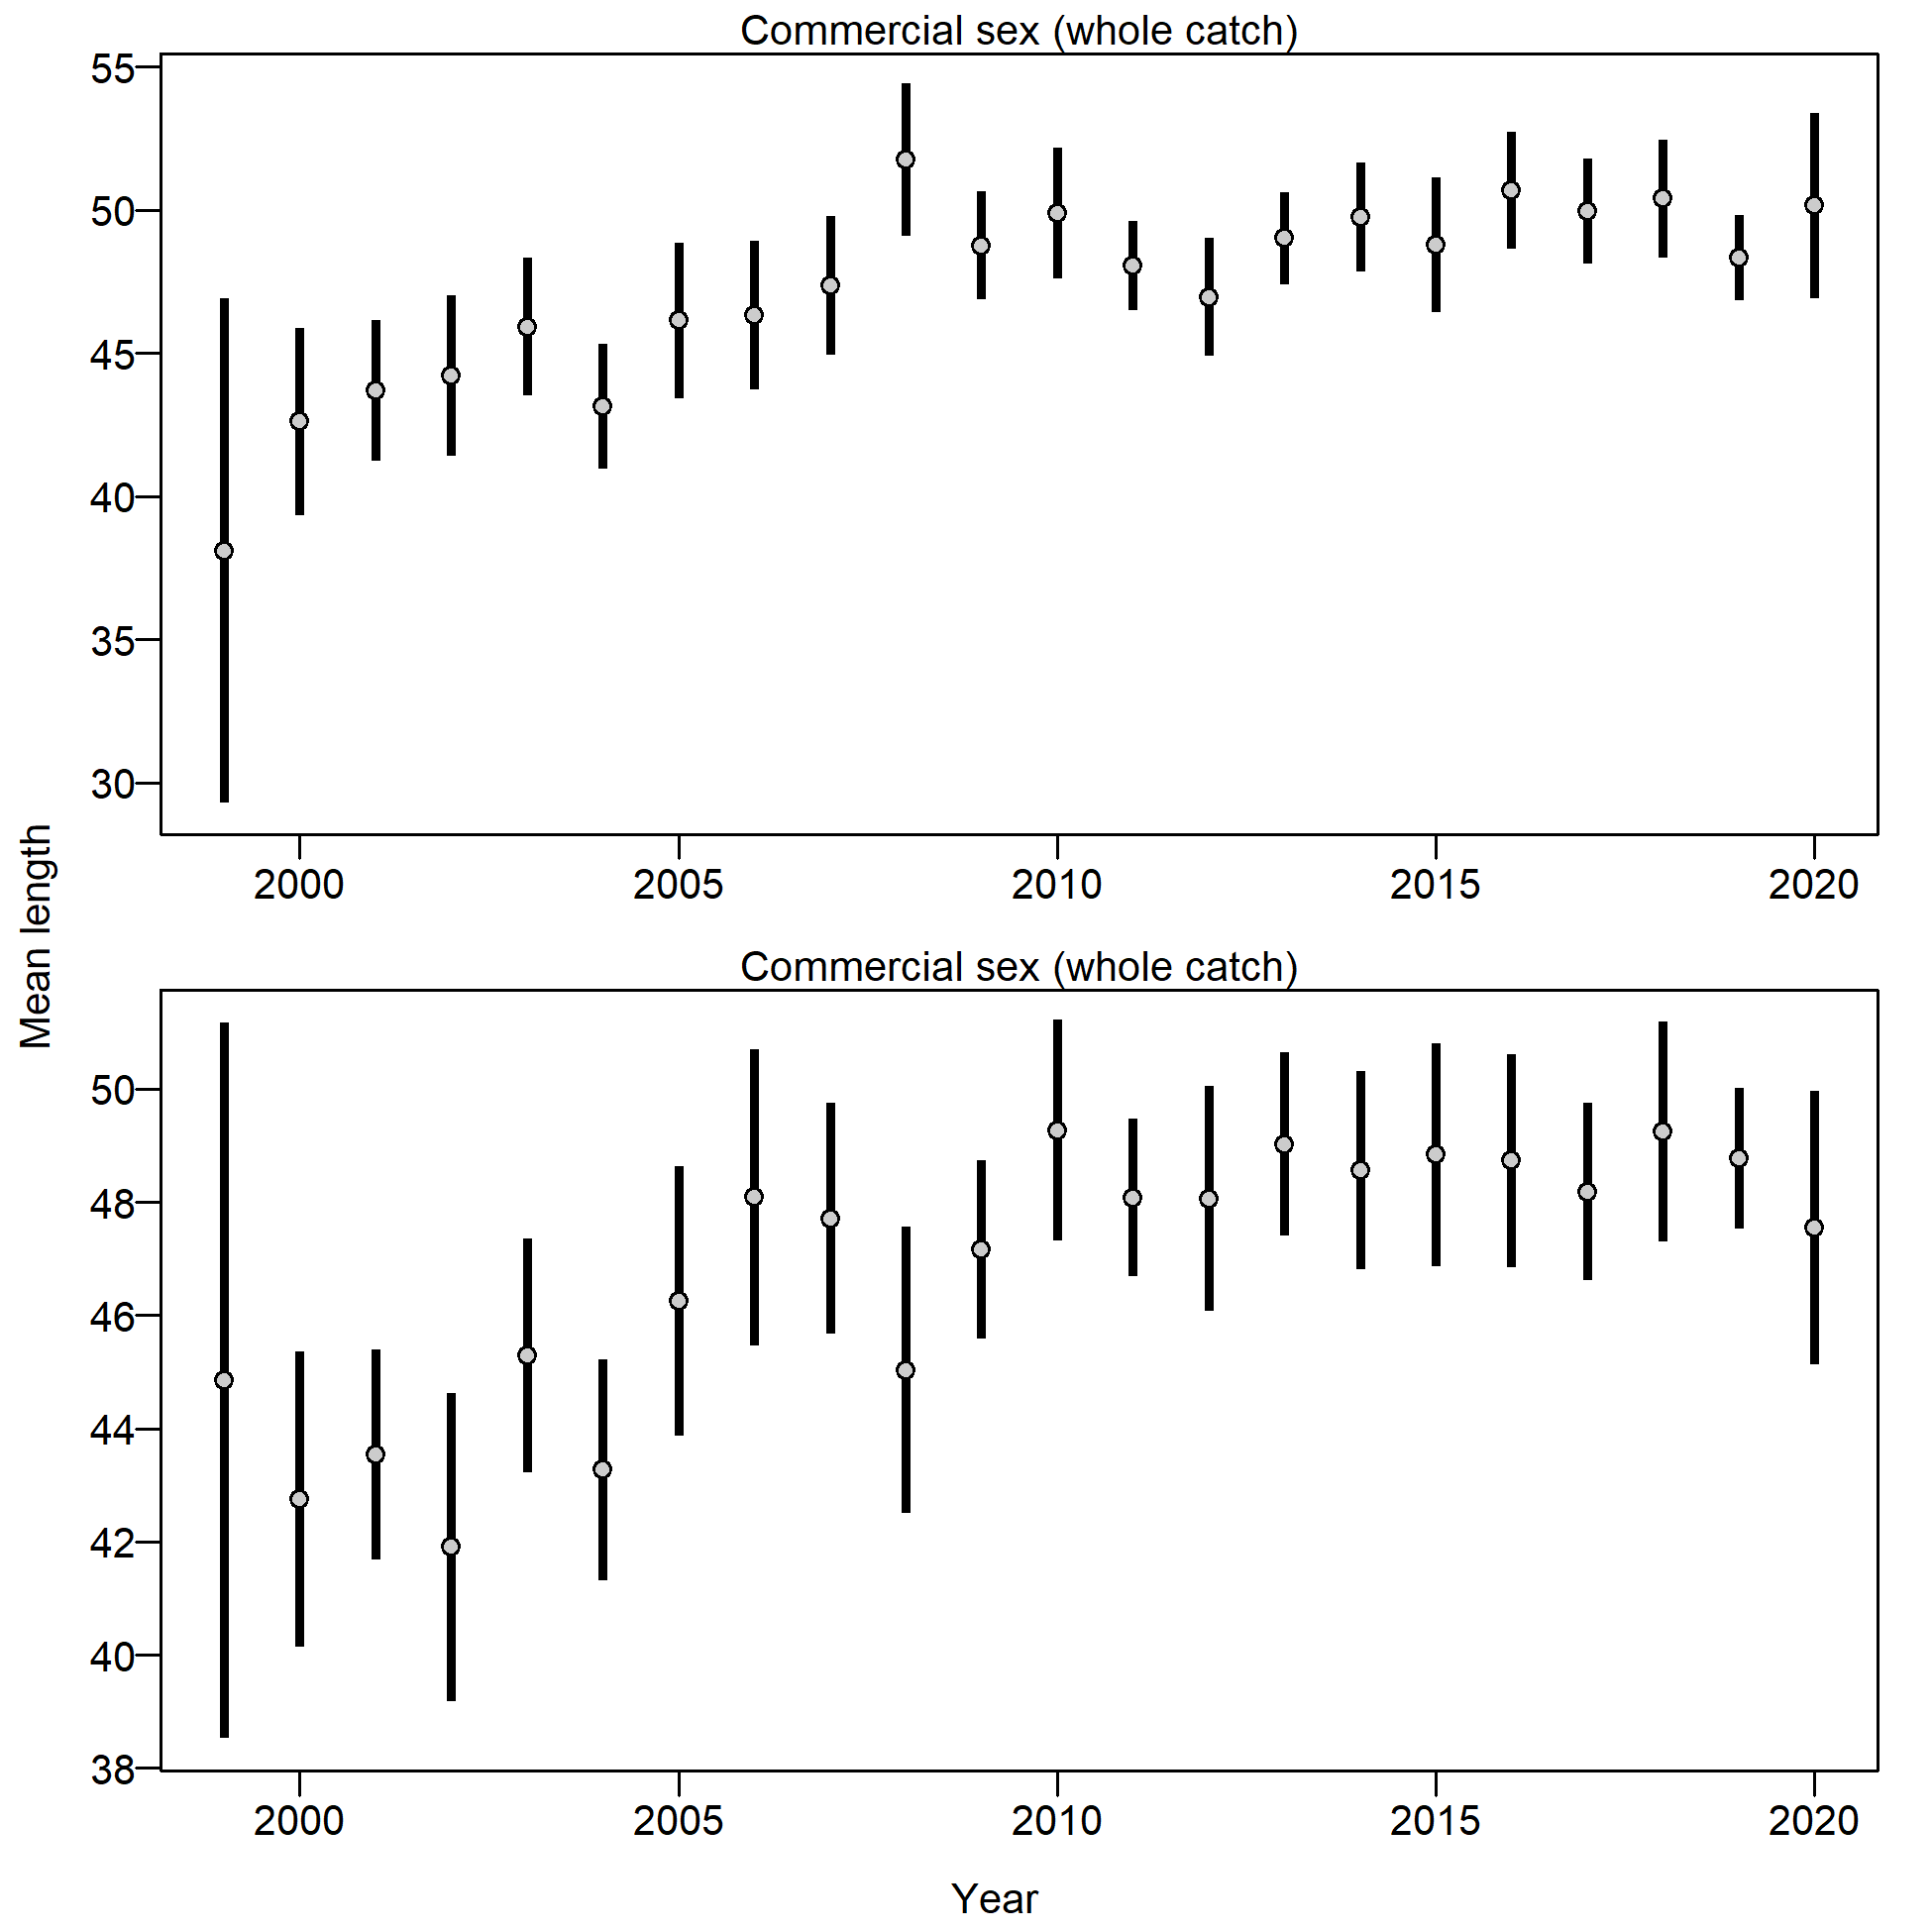
\includegraphics[width=1\textwidth,height=1\textheight]{C:/Users/Jason.Cope/Documents/Github/Vermilion rockfish OR WA assessment 2021/OR/write_up/models/Reference model/plots/comp_lendat_data_weighting_TA1.8_Commercial.png}
\caption{Mean length index from the recreational fishery with 95 percent confidence intervals based on sample sizes and data weighting.\label{fig:rec-mean-len-fit}}
\end{figure}

\tagmcend\tagstructend

\tagstructbegin{tag=Figure,alttext={Aggregated length comps over all years.}}\tagmcbegin{tag=Figure}

\begin{figure}
\centering
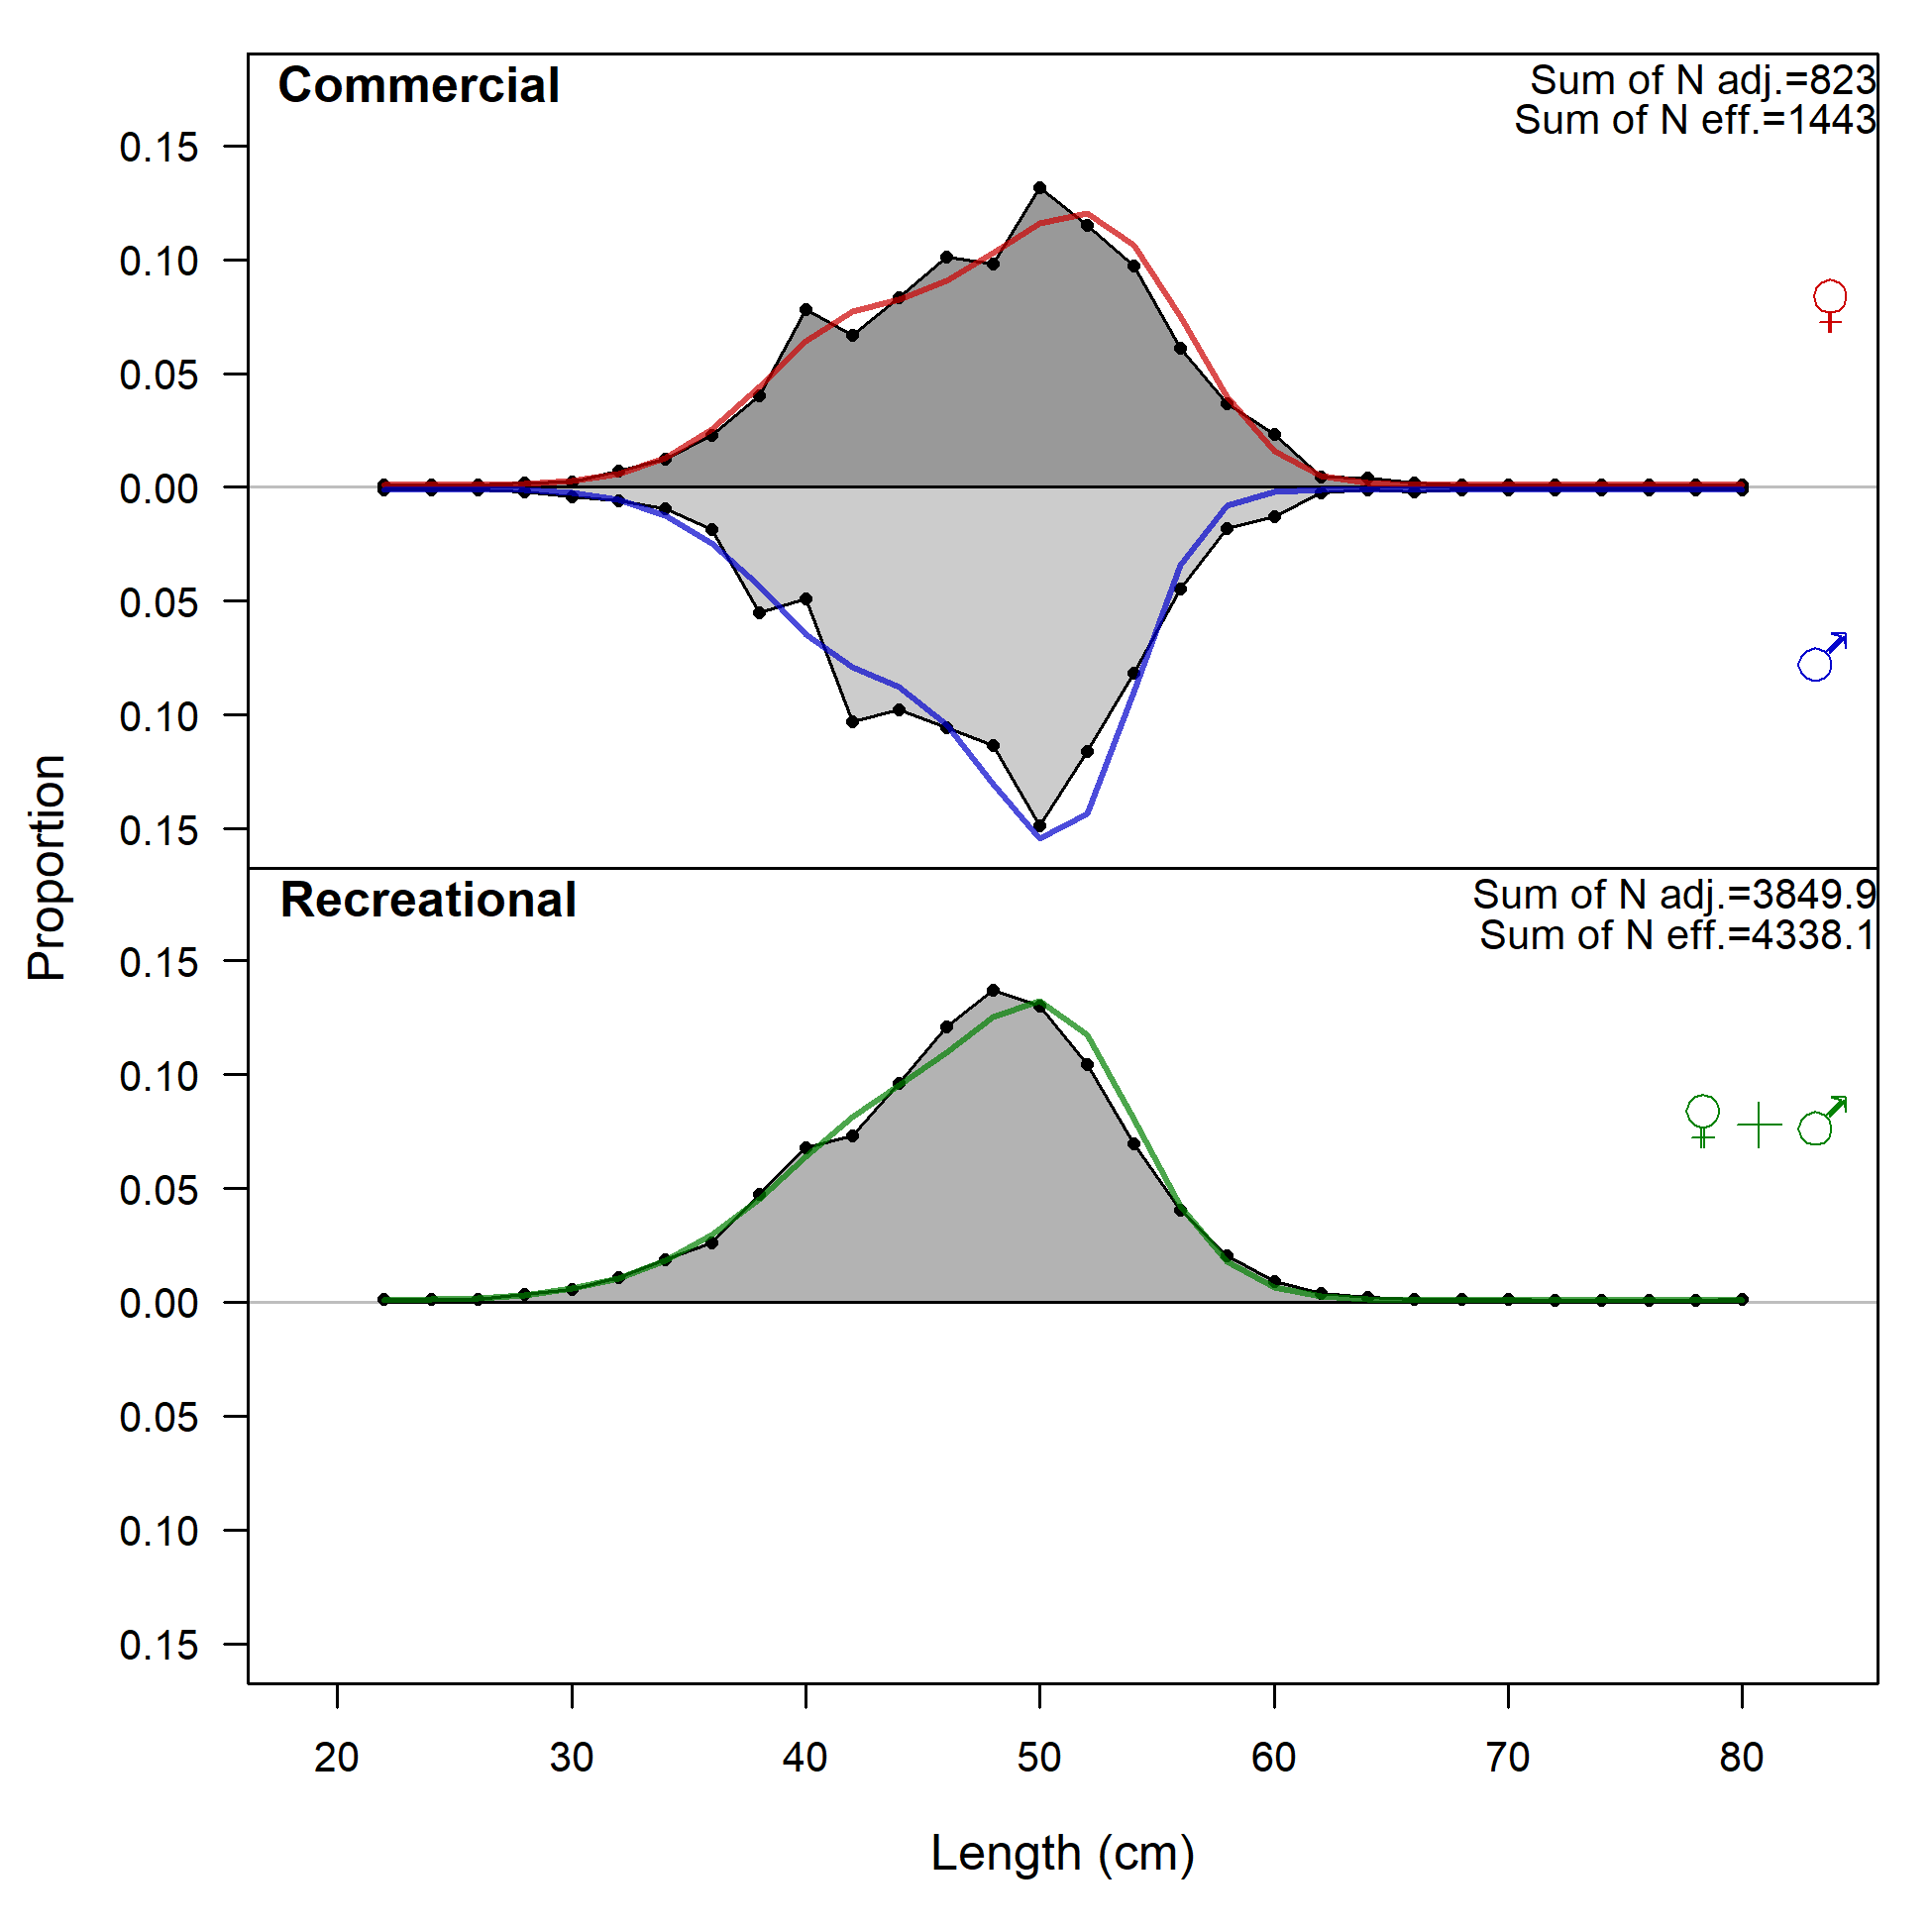
\includegraphics[width=1\textwidth,height=1\textheight]{C:/Users/Jason.Cope/Documents/Github/Vermilion rockfish OR WA assessment 2021/OR/write_up/models/Reference model/plots/comp_lenfit__aggregated_across_time.png}
\caption{Aggregated length comps over all years.\label{fig:agg-len-fit}}
\end{figure}

\tagmcend\tagstructend

\tagstructbegin{tag=Figure,alttext={Mean age from conditional age-at-length data for the Commercial.}}\tagmcbegin{tag=Figure}

\begin{figure}
\centering
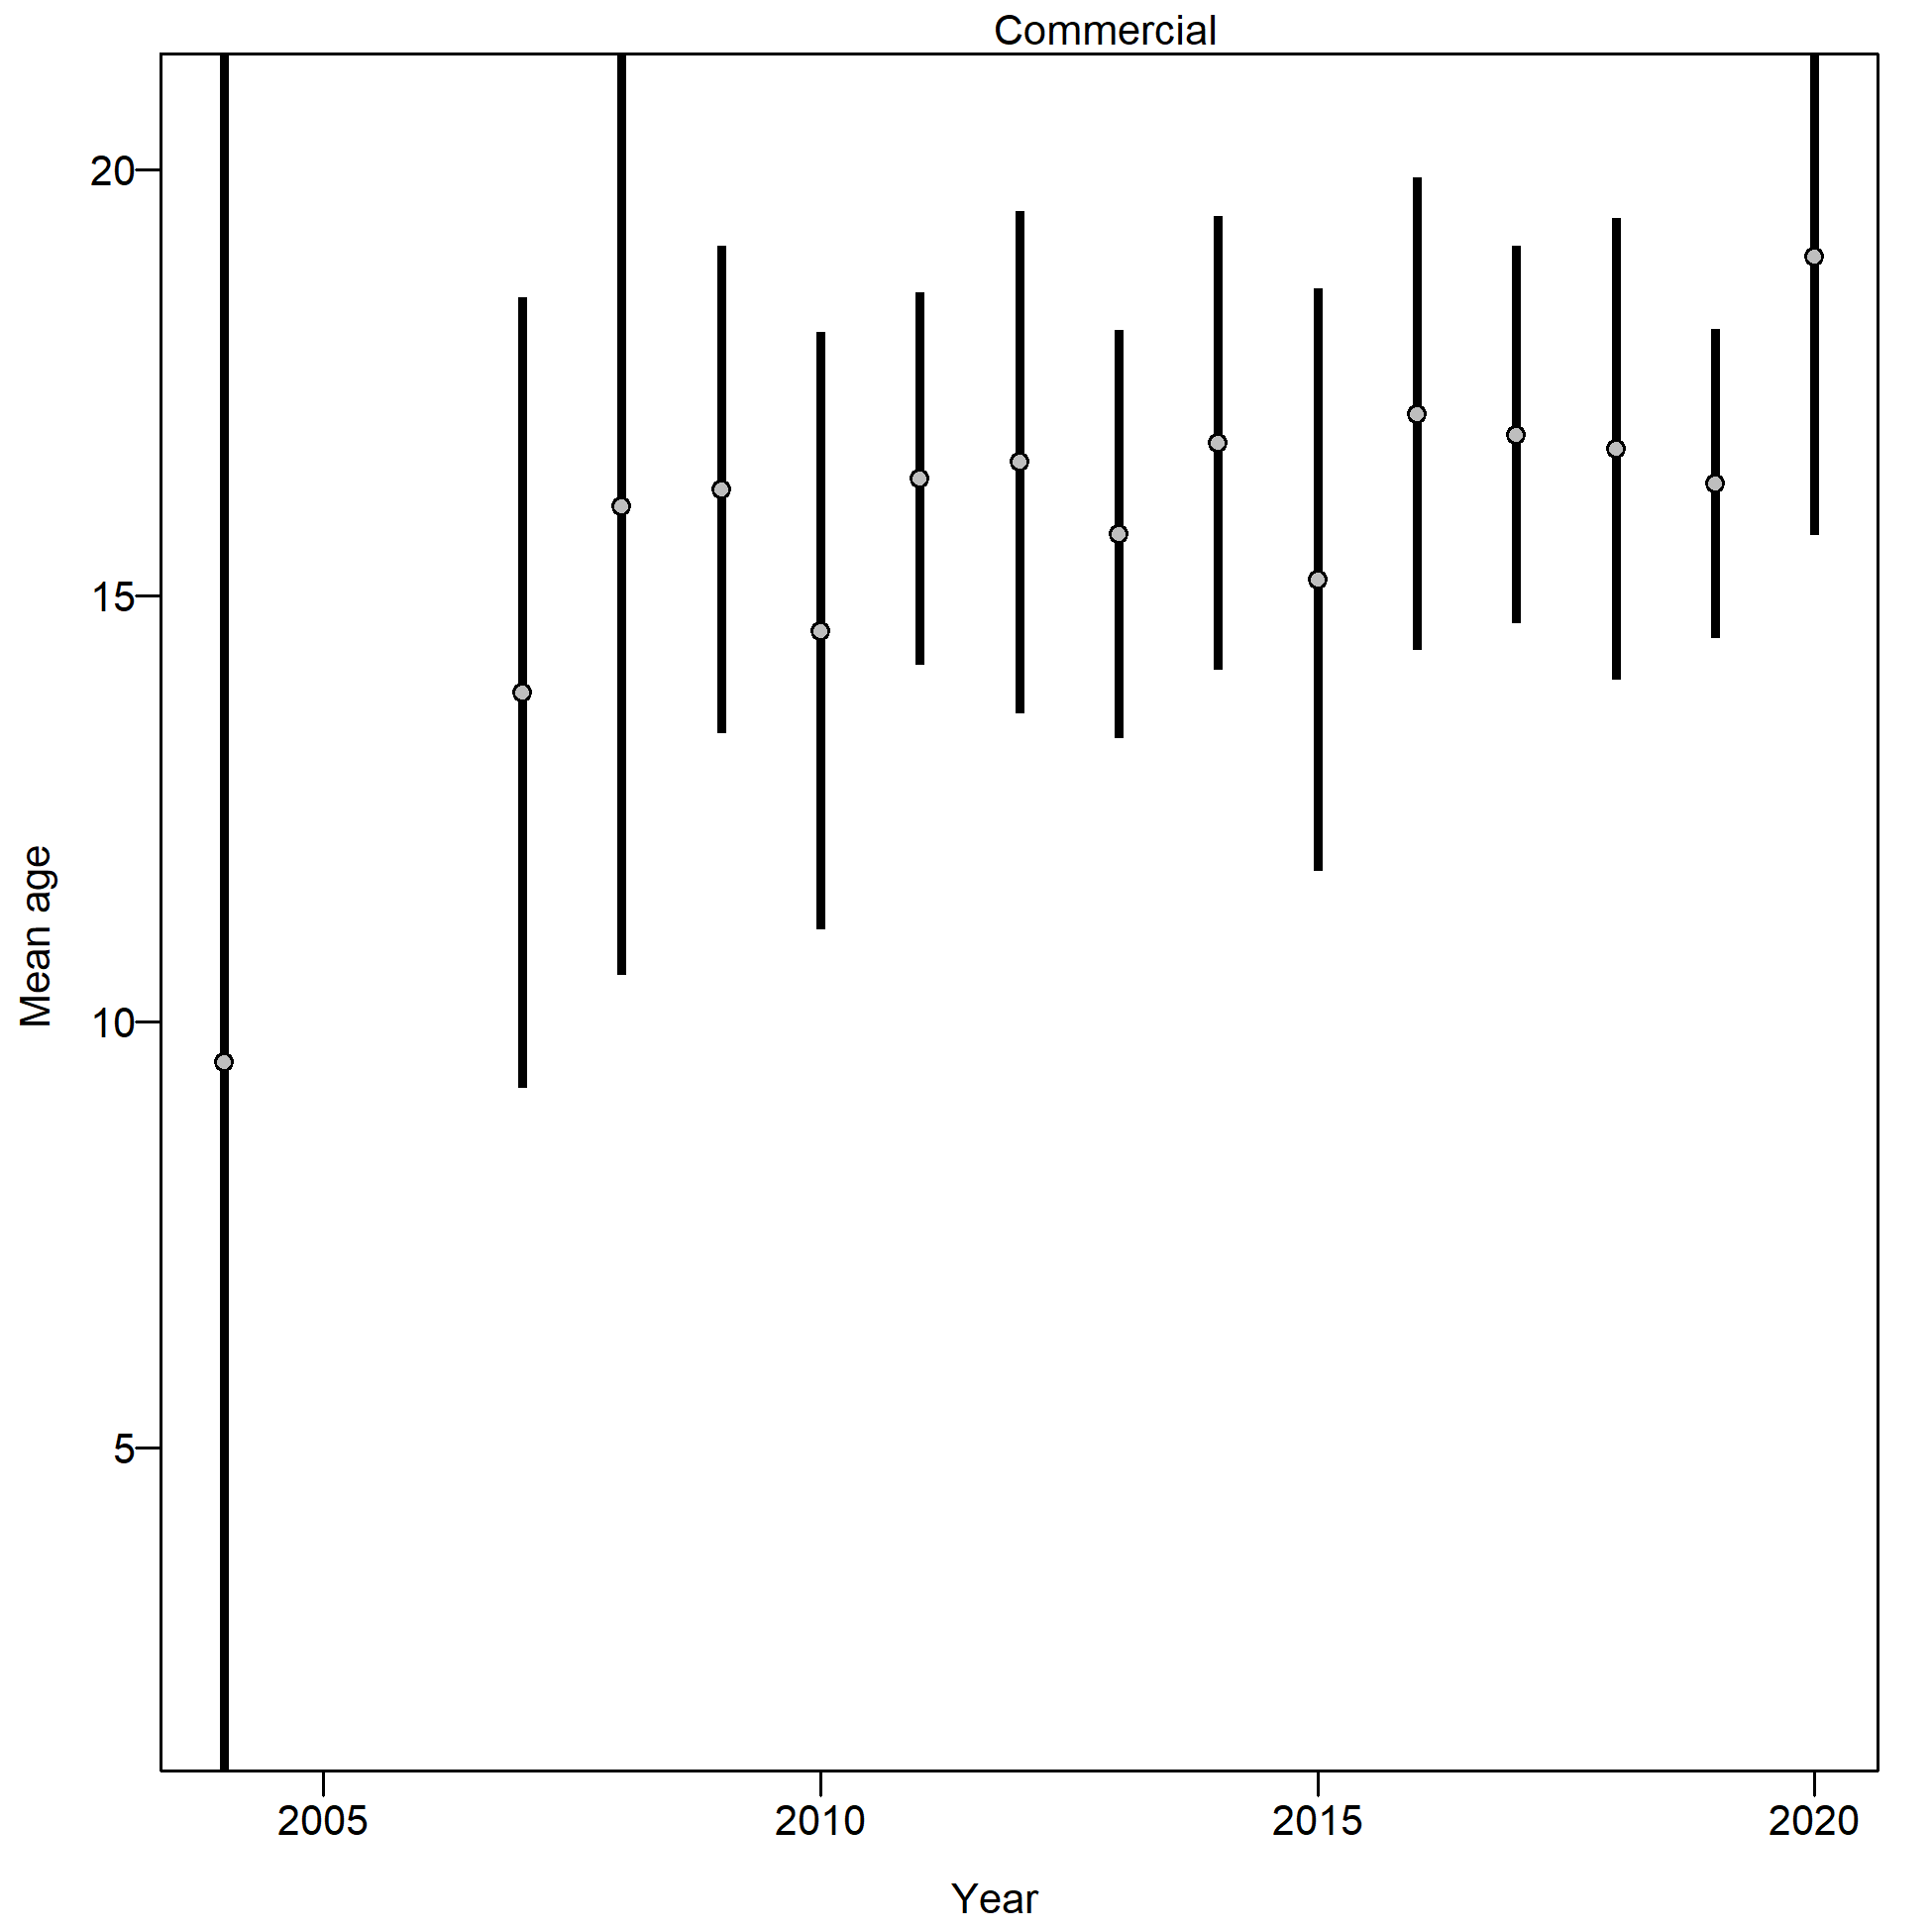
\includegraphics[width=1\textwidth,height=1\textheight]{C:/Users/Jason.Cope/Documents/Github/Vermilion rockfish OR WA assessment 2021/OR/write_up/models/Reference model/plots/comp_condAALdat_data_weighting_TA1.8_condAgeCommercial.png}
\caption{Mean age from conditional age-at-length data for the Commercial.\label{fig:com-mean-caal}}
\end{figure}

\tagmcend\tagstructend

\tagstructbegin{tag=Figure,alttext={Mean age observations from the conditional age-at-length data from the Recreational fishery.}}\tagmcbegin{tag=Figure}

\begin{figure}
\centering
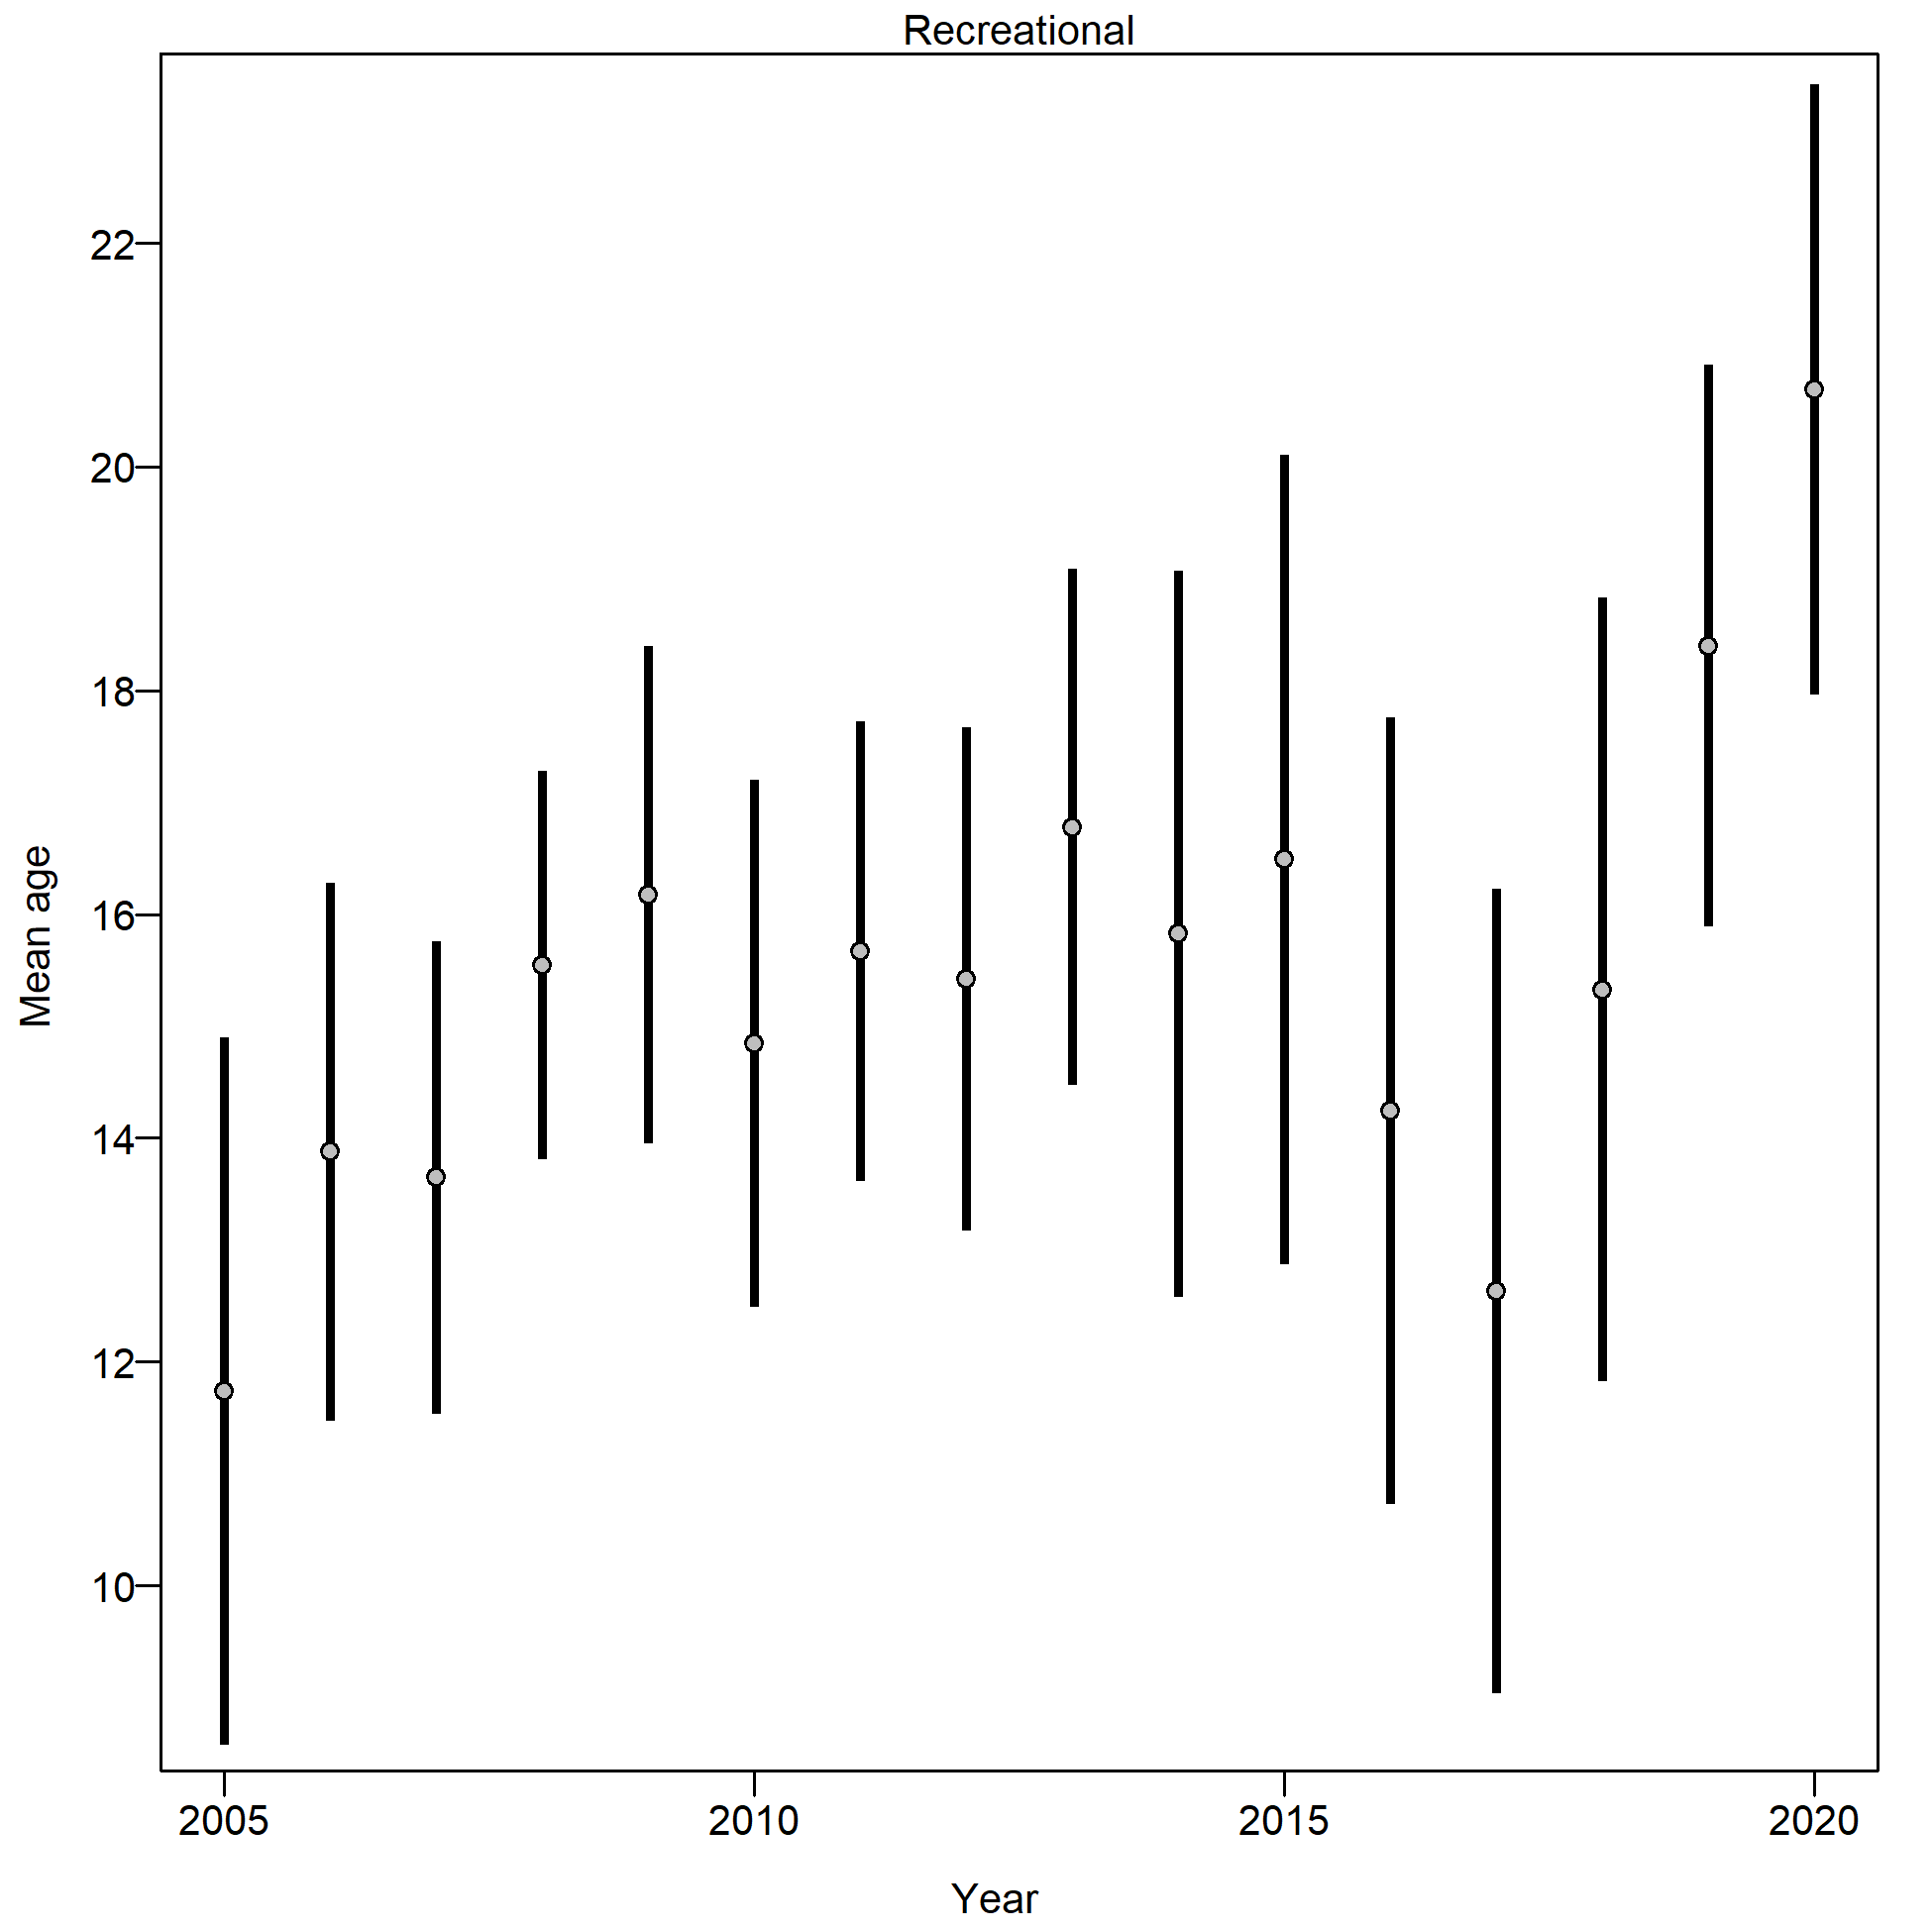
\includegraphics[width=1\textwidth,height=1\textheight]{C:/Users/Jason.Cope/Documents/Github/Vermilion rockfish OR WA assessment 2021/OR/write_up/models/Reference model/plots/comp_condAALdat_data_weighting_TA1.8_condAgeRecreational.png}
\caption{Mean age observations from the conditional age-at-length data from the Recreational fishery.\label{fig:rec-mean-caal}}
\end{figure}

\tagmcend\tagstructend

\tagstructbegin{tag=Figure,alttext={Fit to the ORBS recreational survey index of abundance.}}\tagmcbegin{tag=Figure}

\begin{figure}
\centering
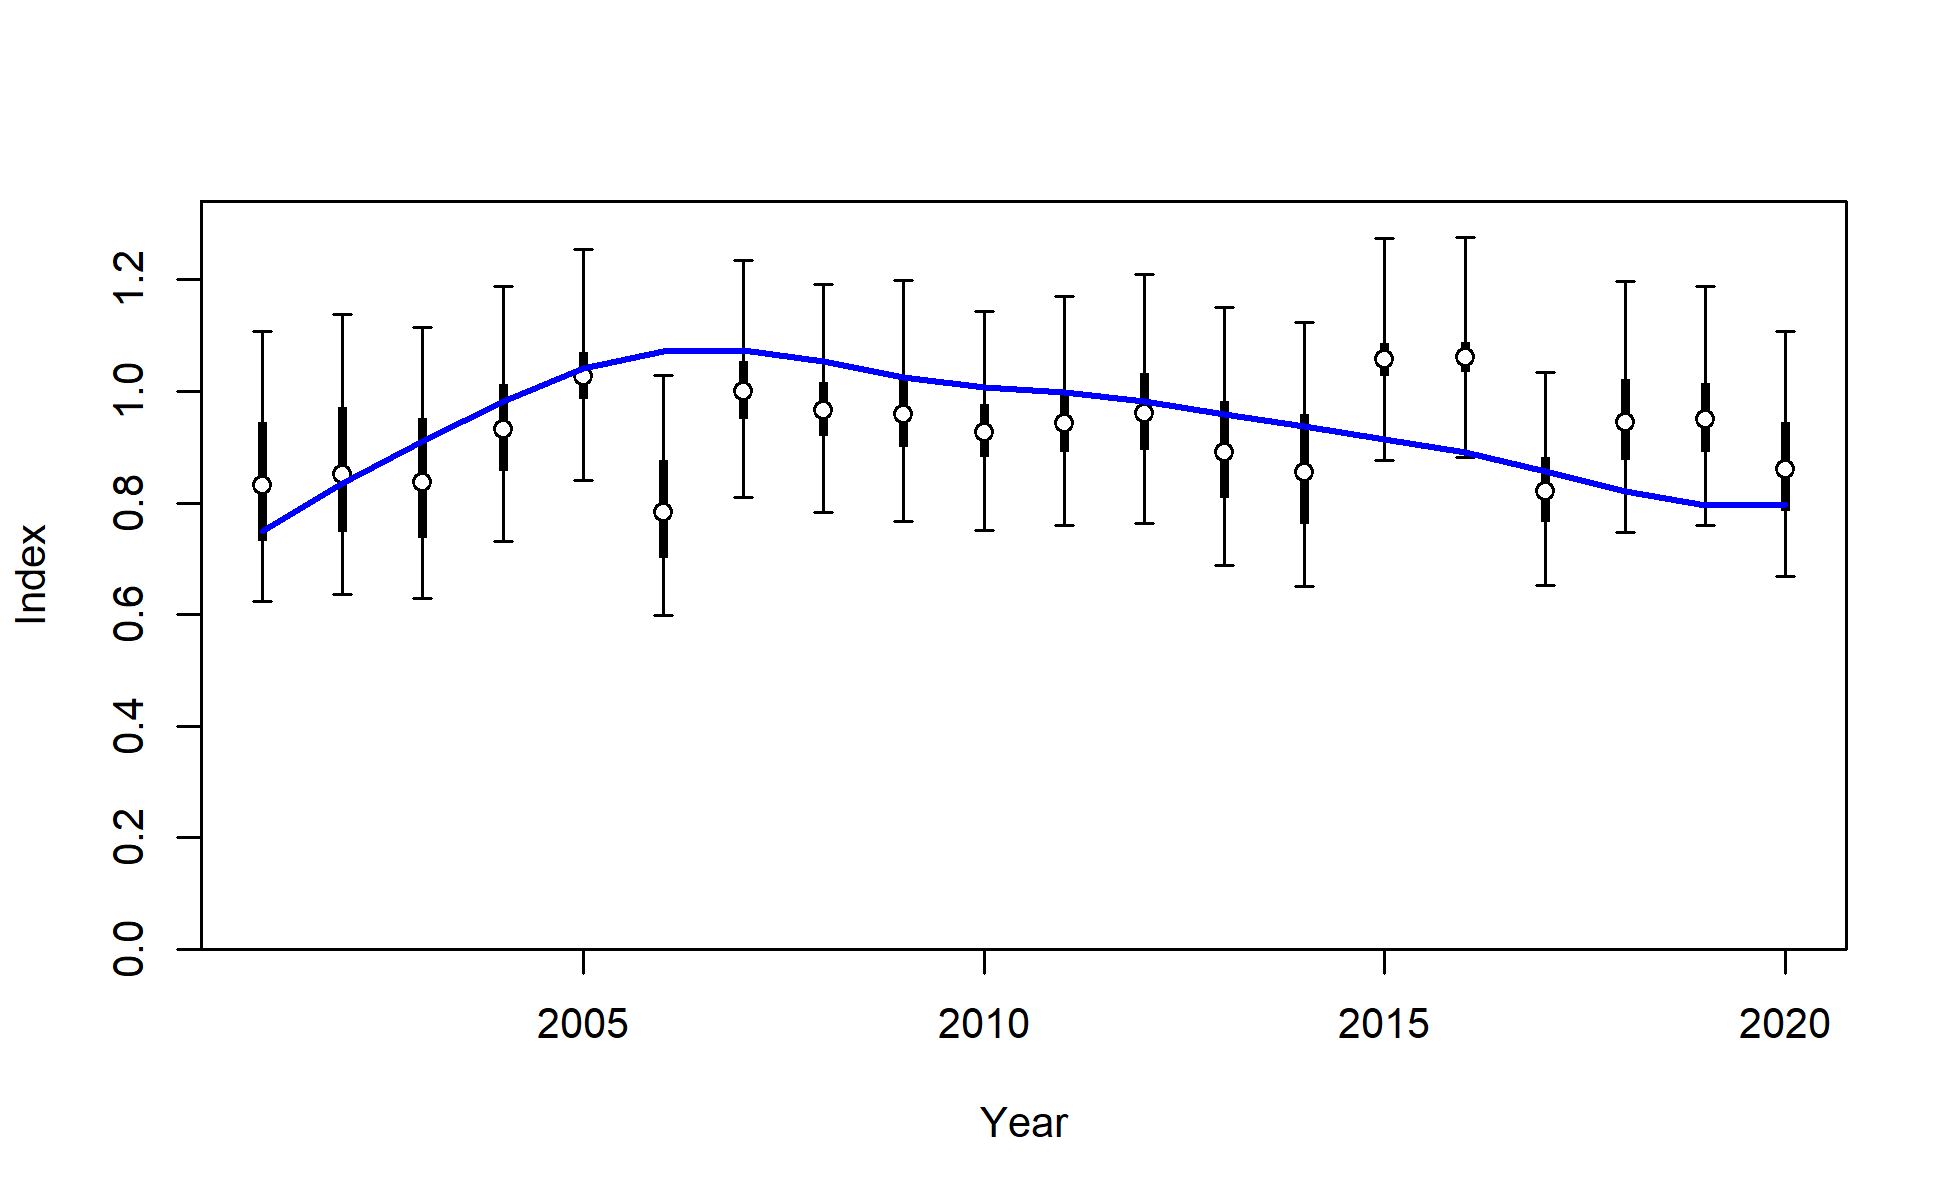
\includegraphics[width=1\textwidth,height=1\textheight]{C:/Users/Jason.Cope/Documents/Github/Vermilion rockfish OR WA assessment 2021/OR/write_up/models/Reference model/plots/index2_cpuefit_Recreational.png}
\caption{Fit to the ORBS recreational survey index of abundance.\label{fig:orbs-index-fit}}
\end{figure}

\tagmcend\tagstructend

\tagstructbegin{tag=Figure,alttext={Length-based selectivity curves for the commercial and recreational fisheries.}}\tagmcbegin{tag=Figure}

\begin{figure}
\centering
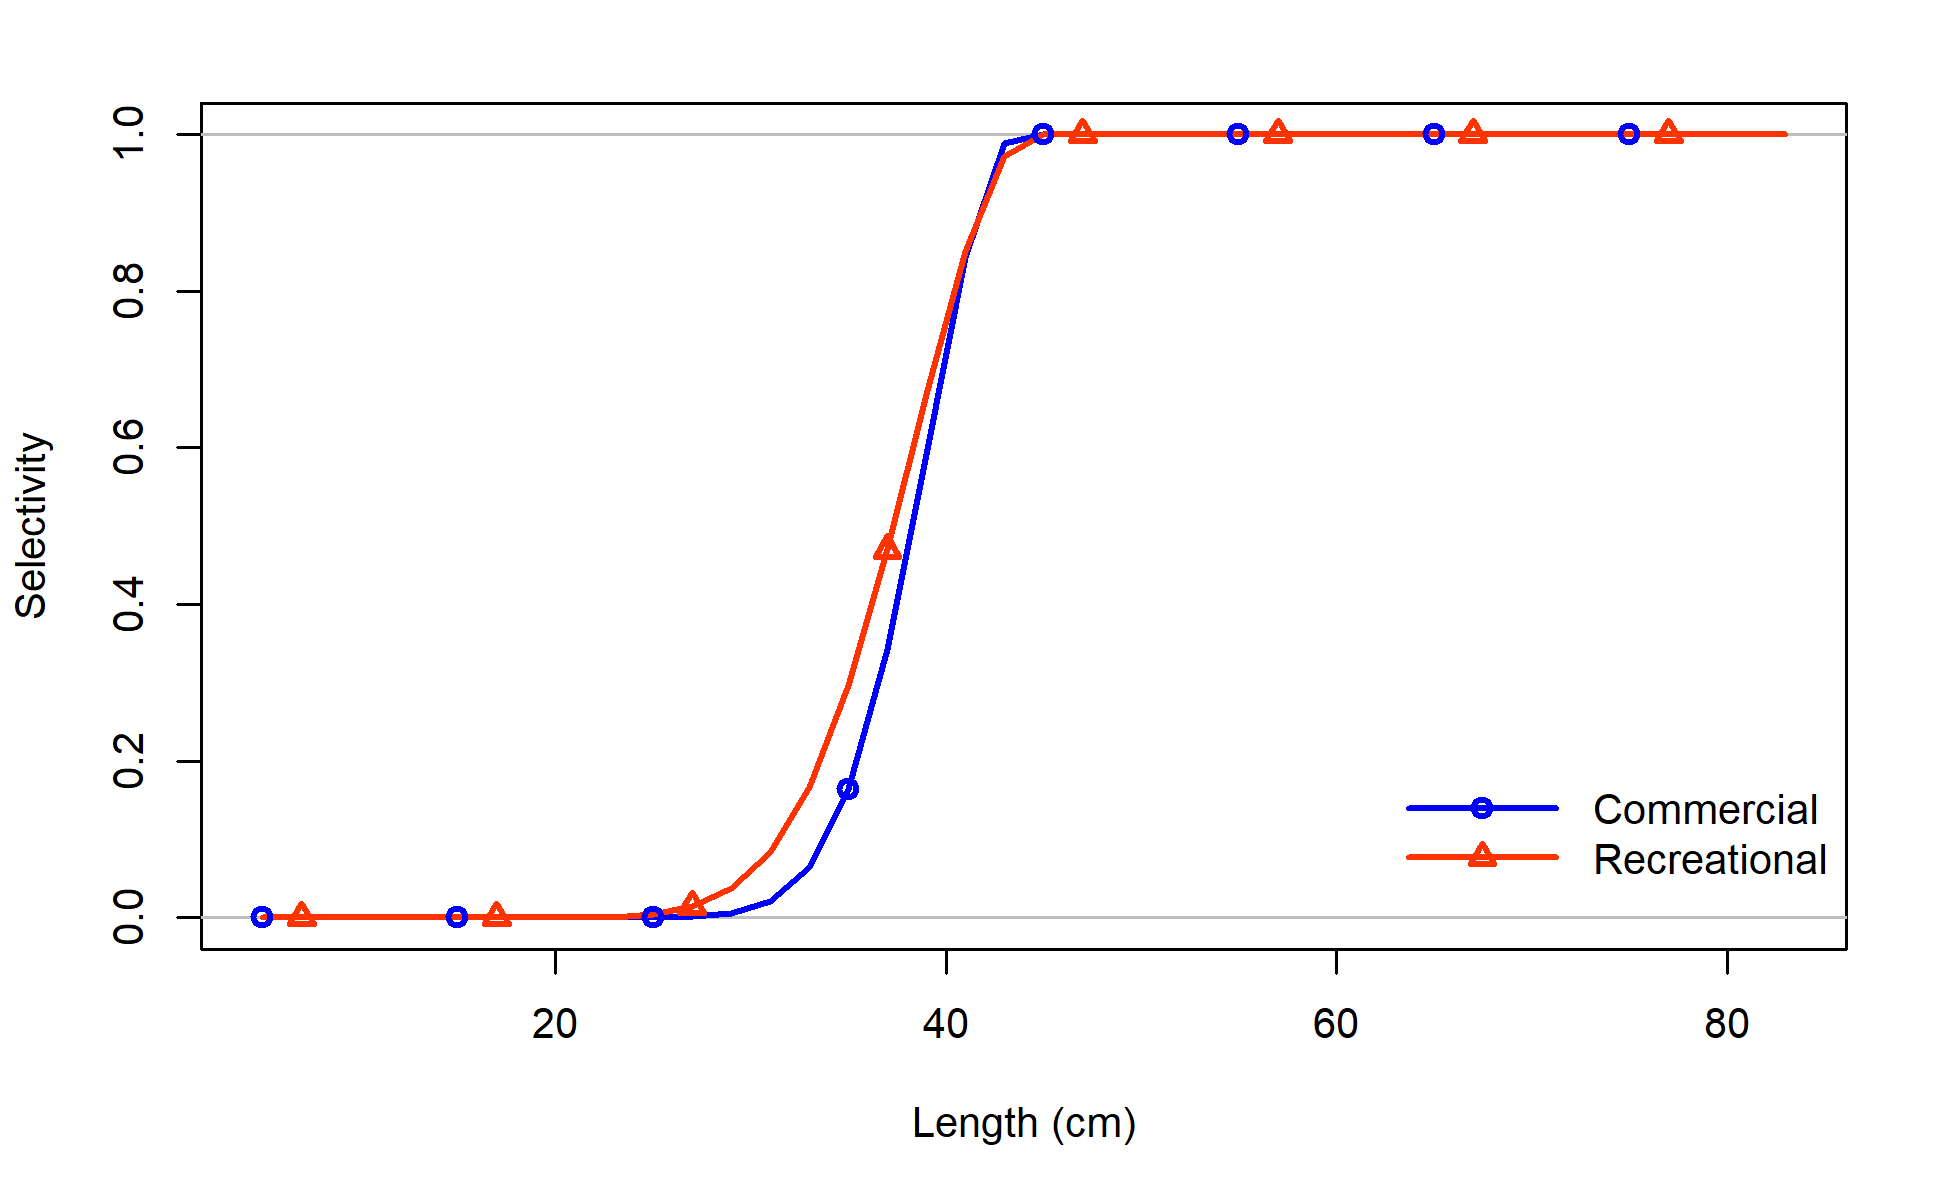
\includegraphics[width=1\textwidth,height=1\textheight]{C:/Users/Jason.Cope/Documents/Github/Vermilion rockfish OR WA assessment 2021/OR/write_up/models/Reference model/plots/sel01_multiple_fleets_length1.png}
\caption{Length-based selectivity curves for the commercial and recreational fisheries.\label{fig:fleet_selectivity}}
\end{figure}

\tagmcend\tagstructend

\clearpage

\tagstructbegin{tag=H1}\tagmcbegin{tag=H1}

\hypertarget{appendix-a.-summary-of-california-management-measures}{%
\section{Appendix A. Summary of California Management Measures}\label{appendix-a.-summary-of-california-management-measures}}

\leavevmode\tagmcend\tagstructend

\tagstructbegin{tag=P}\tagmcbegin{tag=P}

Appendix A can be found in the separate file ``California Nearshore Regulation History.pdf.''

\leavevmode\tagmcend\tagstructend\par

\tagstructbegin{tag=H1}\tagmcbegin{tag=H1}

\hypertarget{appendix-b.-detailed-fit-to-length-composition-data}{%
\section{Appendix B. Detailed Fit to Length Composition Data}\label{appendix-b.-detailed-fit-to-length-composition-data}}

\leavevmode\tagmcend\tagstructend

\tagstructbegin{tag=Figure,alttext={Length comps, whole catch, Commercial.<br><br>'N adj.' is the input sample size after data-weighting adjustment. N eff. is the calculated effective sample size used in the McAllister-Ianelli tuning method..}}\tagmcbegin{tag=Figure}

\begin{figure}
\centering
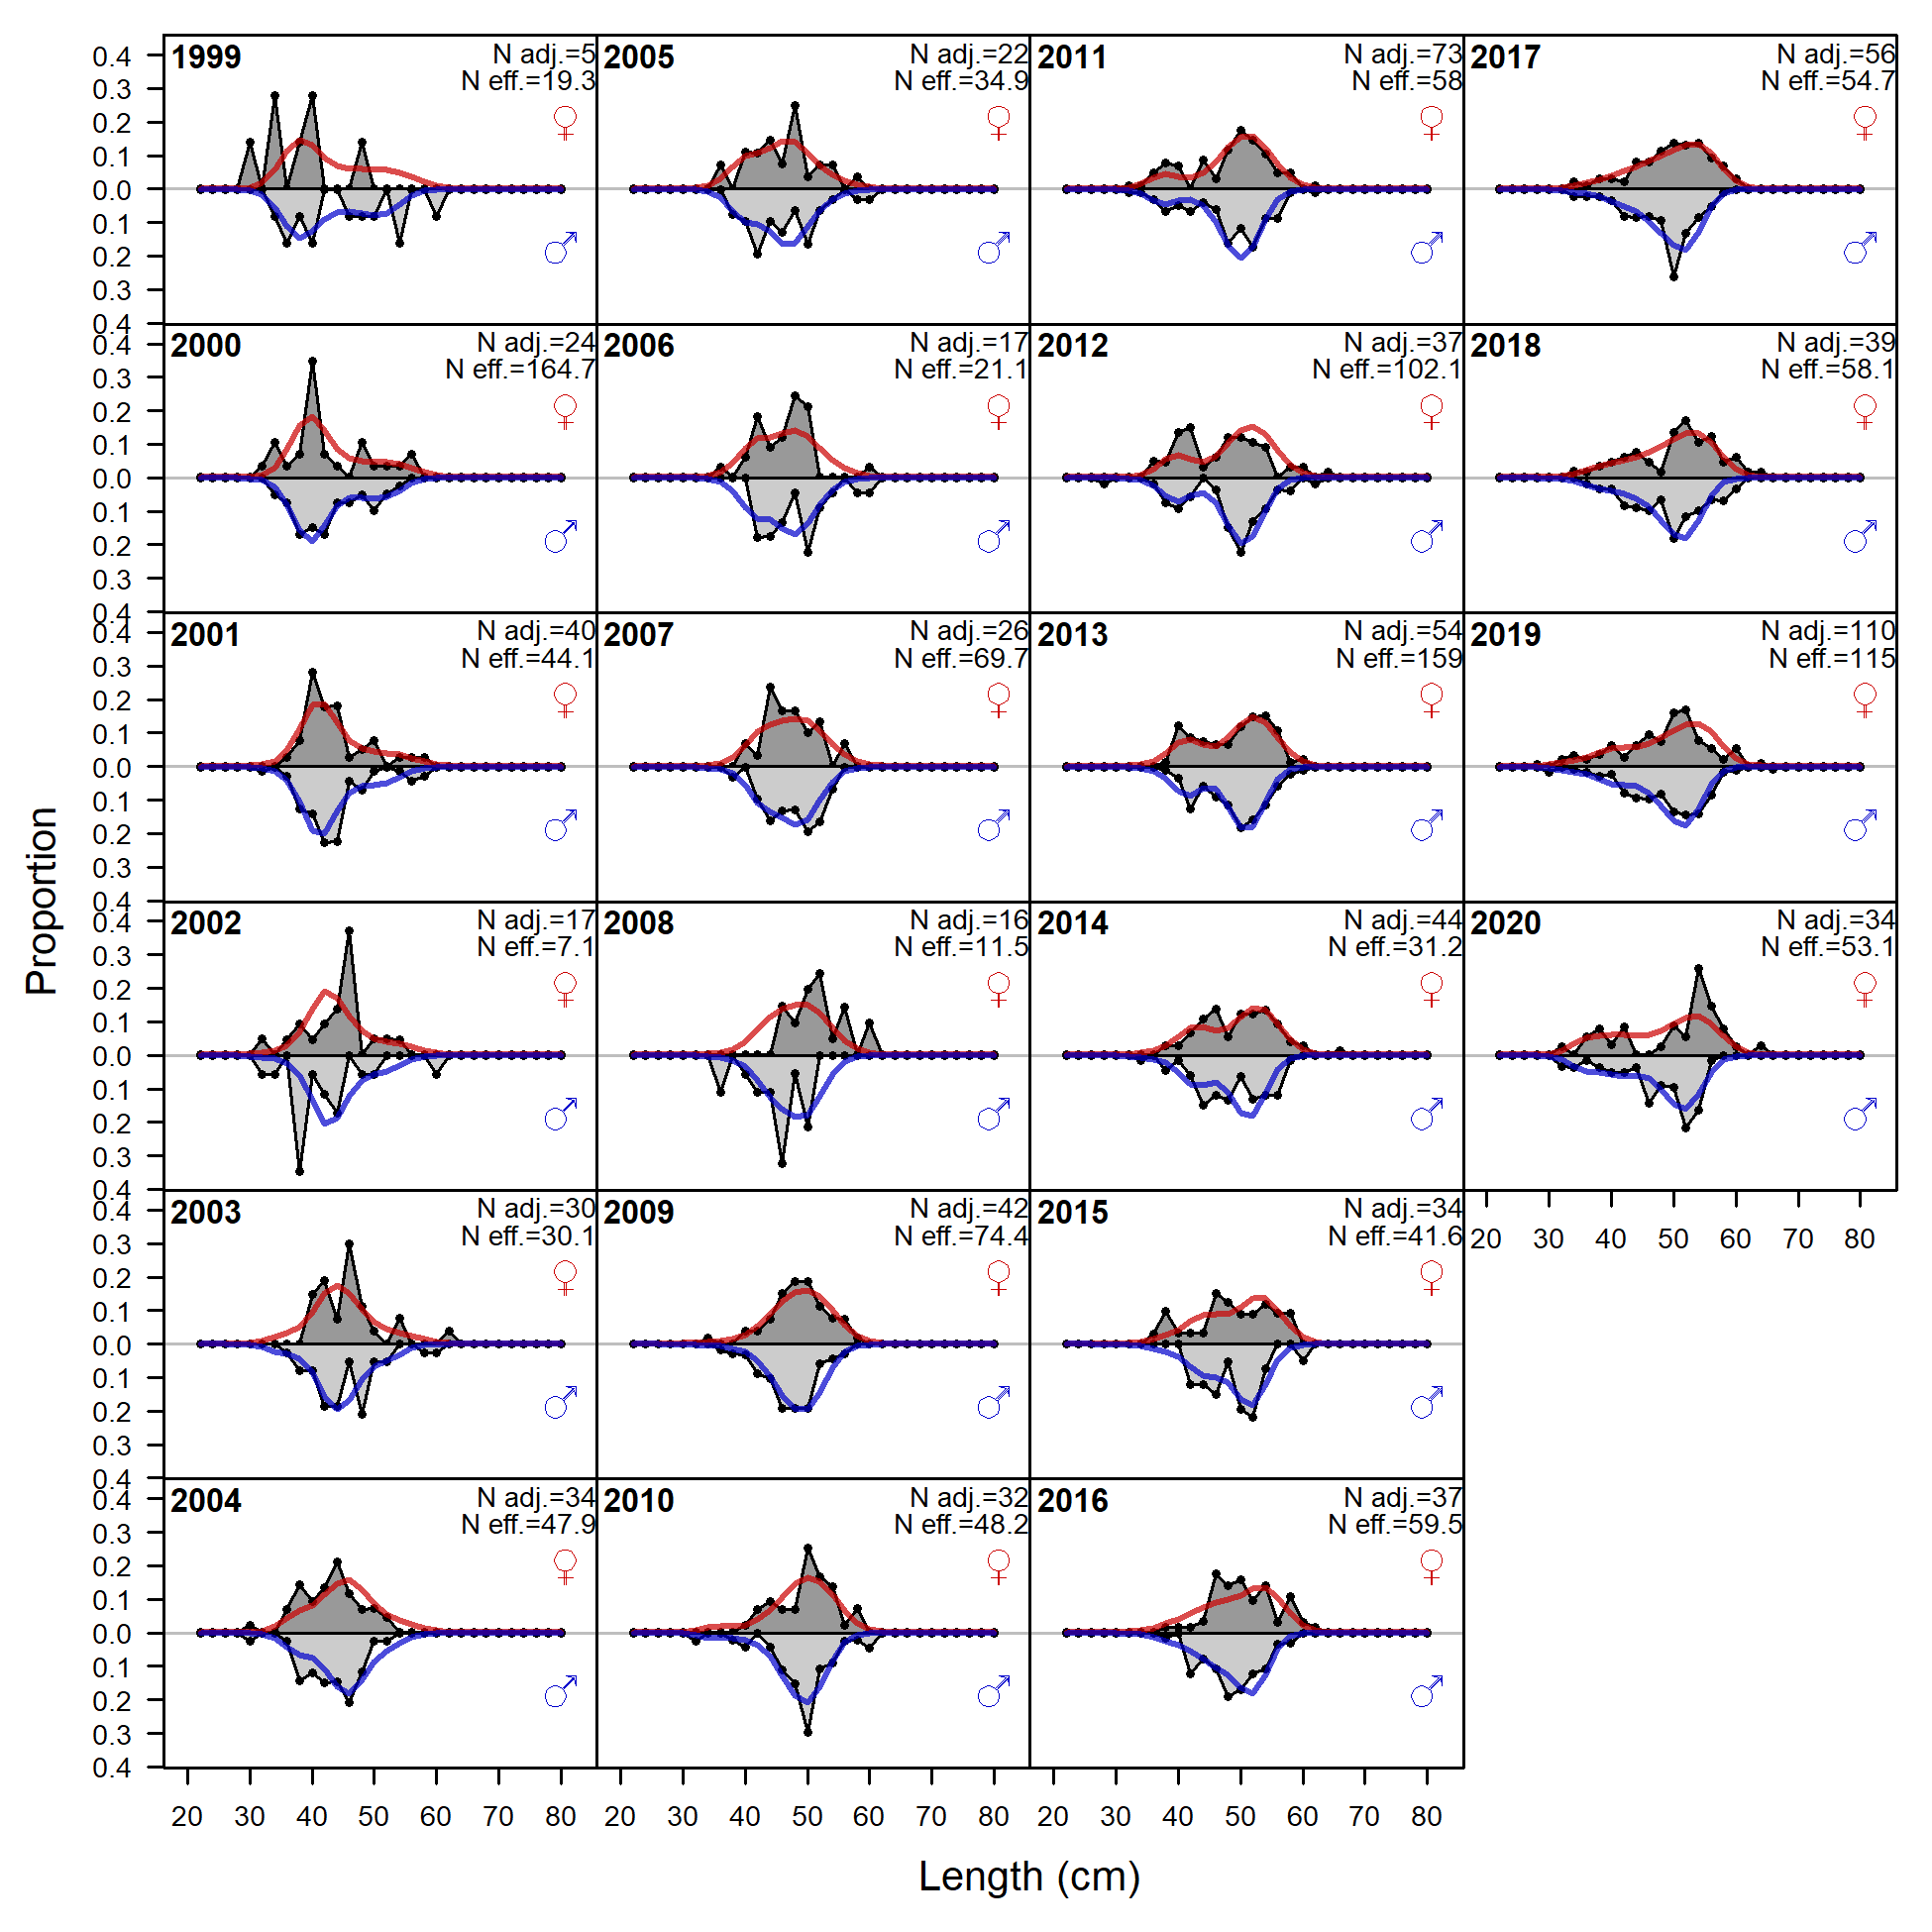
\includegraphics[width=1\textwidth,height=1\textheight]{C:/Users/Jason.Cope/Documents/Github/Vermilion rockfish OR WA assessment 2021/OR/write_up/models/Reference model/plots/comp_lenfit_flt1mkt0.png}
\caption{Length comps, whole catch, Commercial.`N adj.' is the input sample size after data-weighting adjustment. N eff. is the calculated effective sample size used in the McAllister-Ianelli tuning method..\label{fig:comp_lenfit_flt1mkt0}}
\end{figure}

\tagmcend\tagstructend

\tagstructbegin{tag=Figure,alttext={Length comps, whole catch, Recreational (plot 1 of 2).<br><br>'N adj.' is the input sample size after data-weighting adjustment. N eff. is the calculated effective sample size used in the McAllister-Ianelli tuning method..}}\tagmcbegin{tag=Figure}

\begin{figure}
\centering
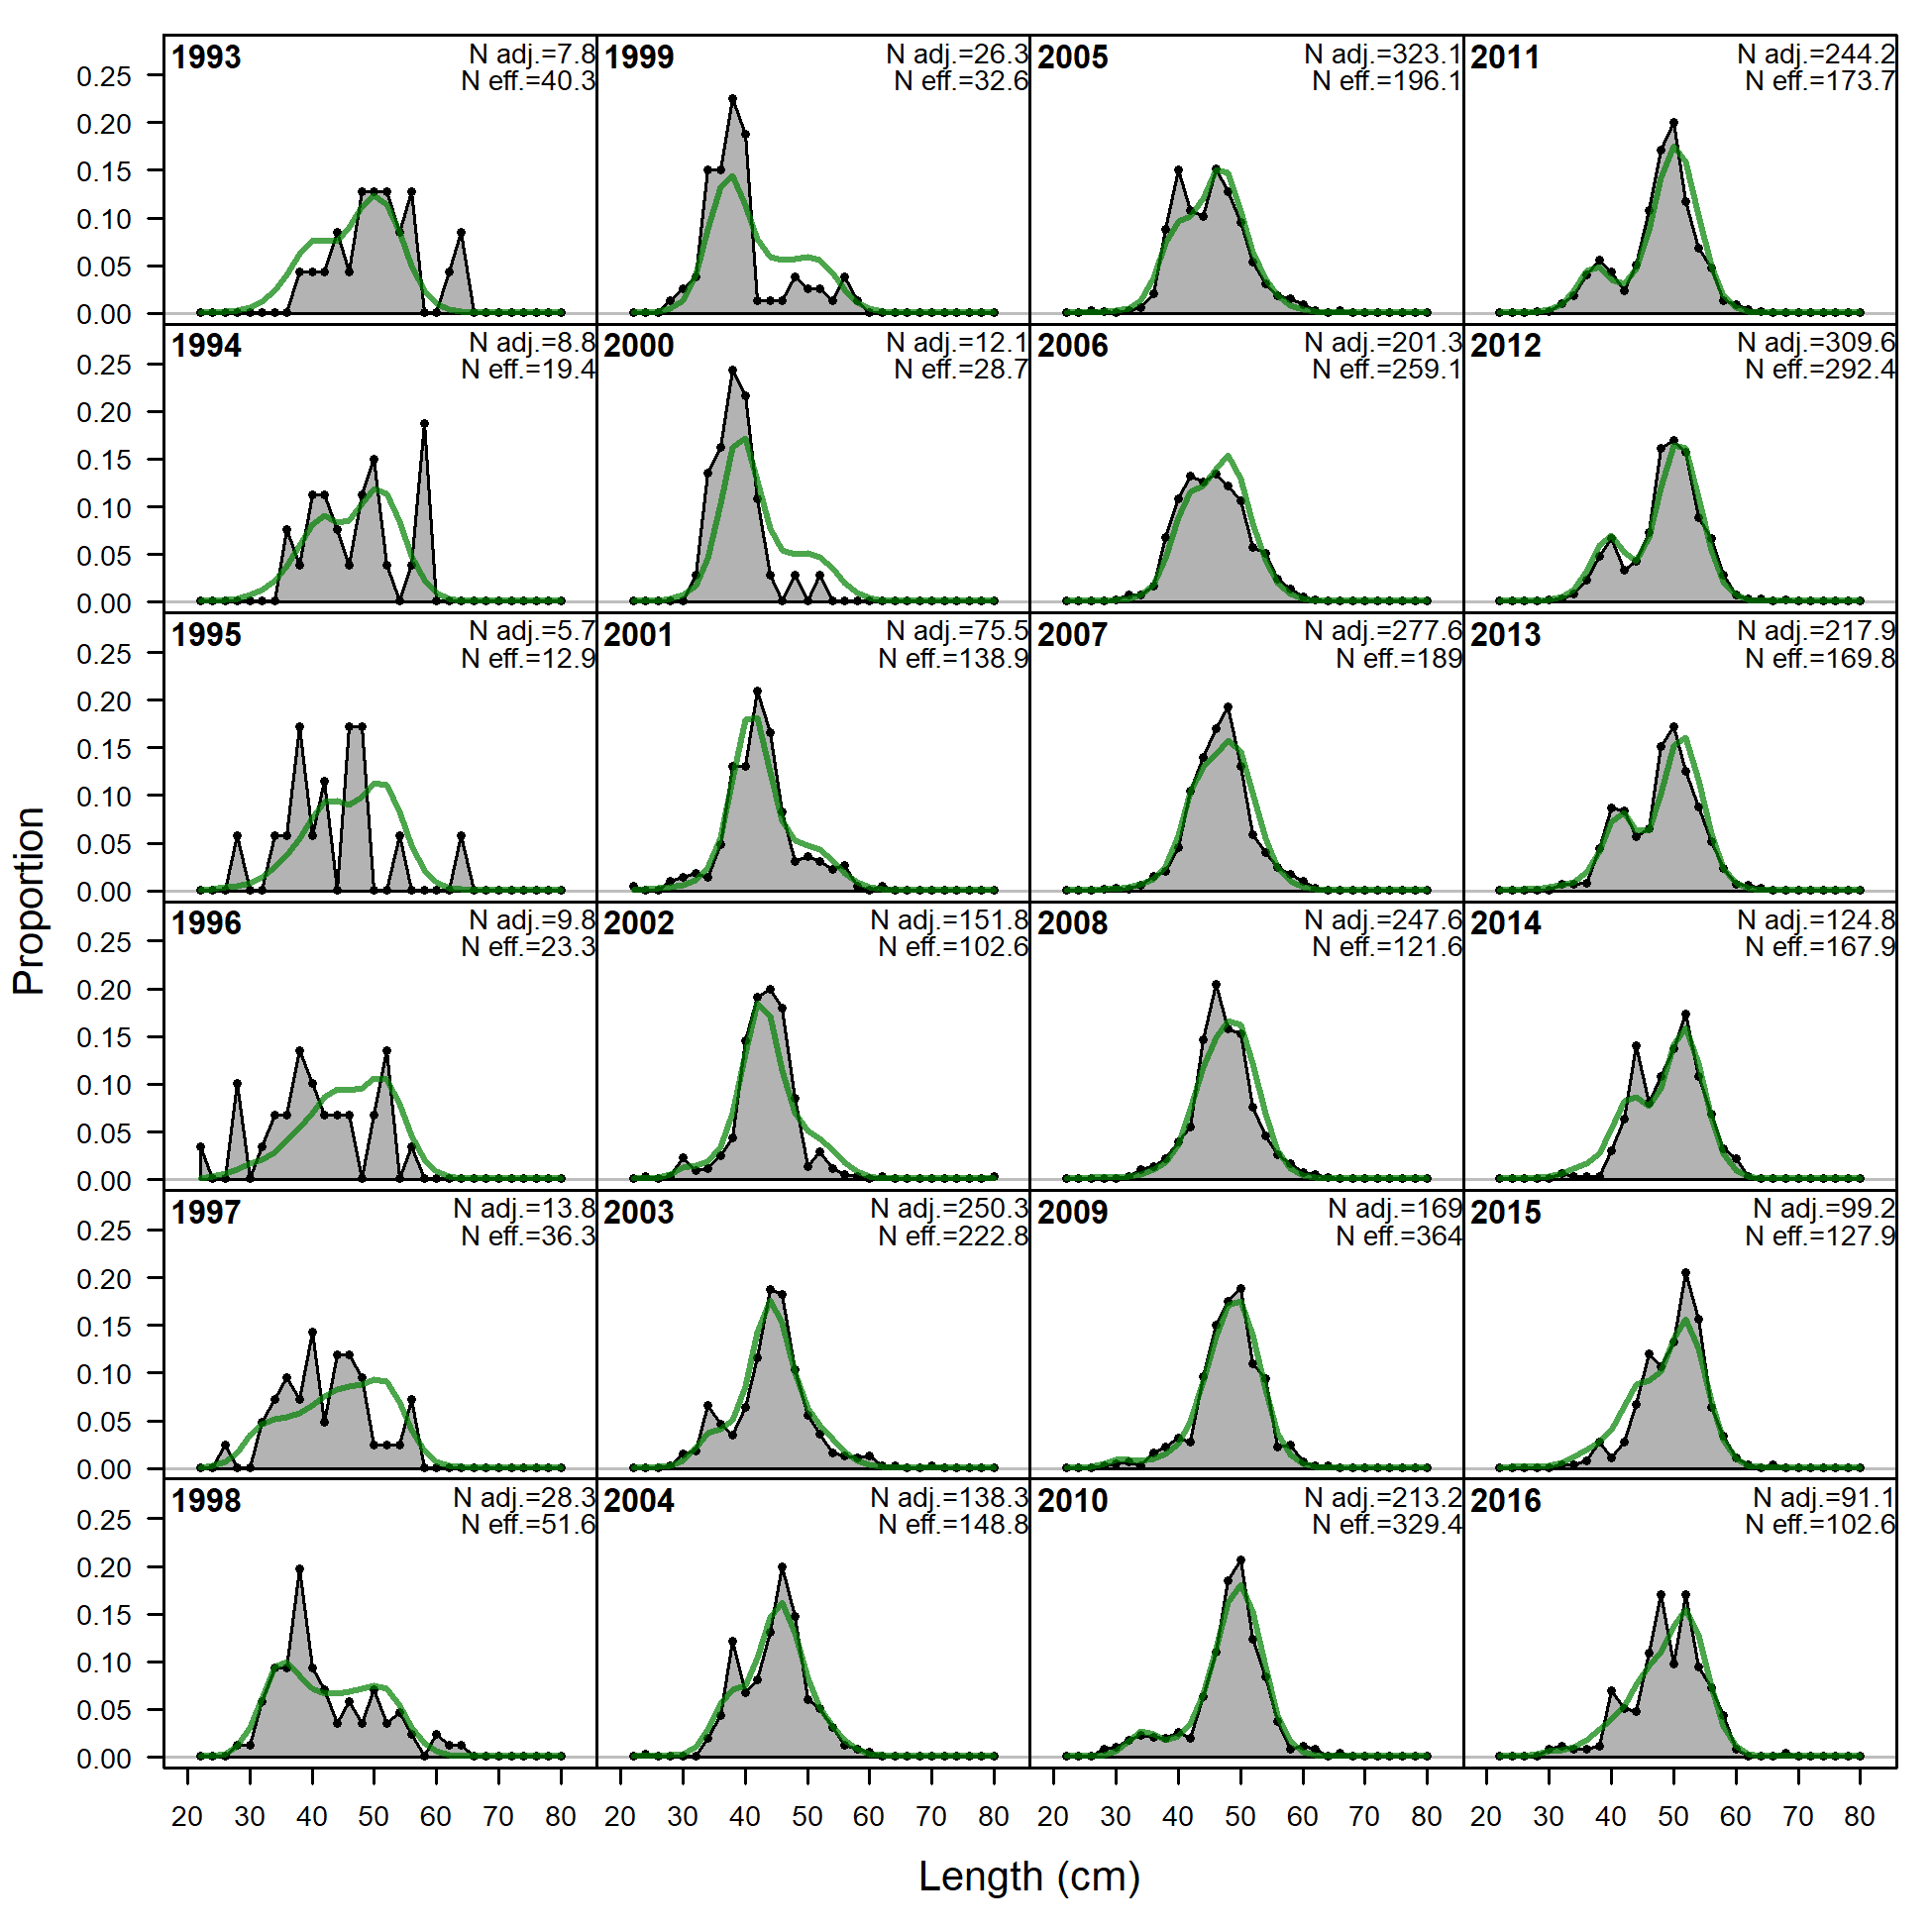
\includegraphics[width=1\textwidth,height=1\textheight]{C:/Users/Jason.Cope/Documents/Github/Vermilion rockfish OR WA assessment 2021/OR/write_up/models/Reference model/plots/comp_lenfit_flt2mkt0_page1.png}
\caption{Length comps, whole catch, Recreational (plot 1 of 2).`N adj.' is the input sample size after data-weighting adjustment. N eff. is the calculated effective sample size used in the McAllister-Ianelli tuning method..\label{fig:comp_lenfit_flt2mkt0_page1}}
\end{figure}

\tagmcend\tagstructend

\tagstructbegin{tag=Figure,alttext={Length comps, whole catch, Recreational (plot 2 of 2).}}\tagmcbegin{tag=Figure}

\begin{figure}
\centering
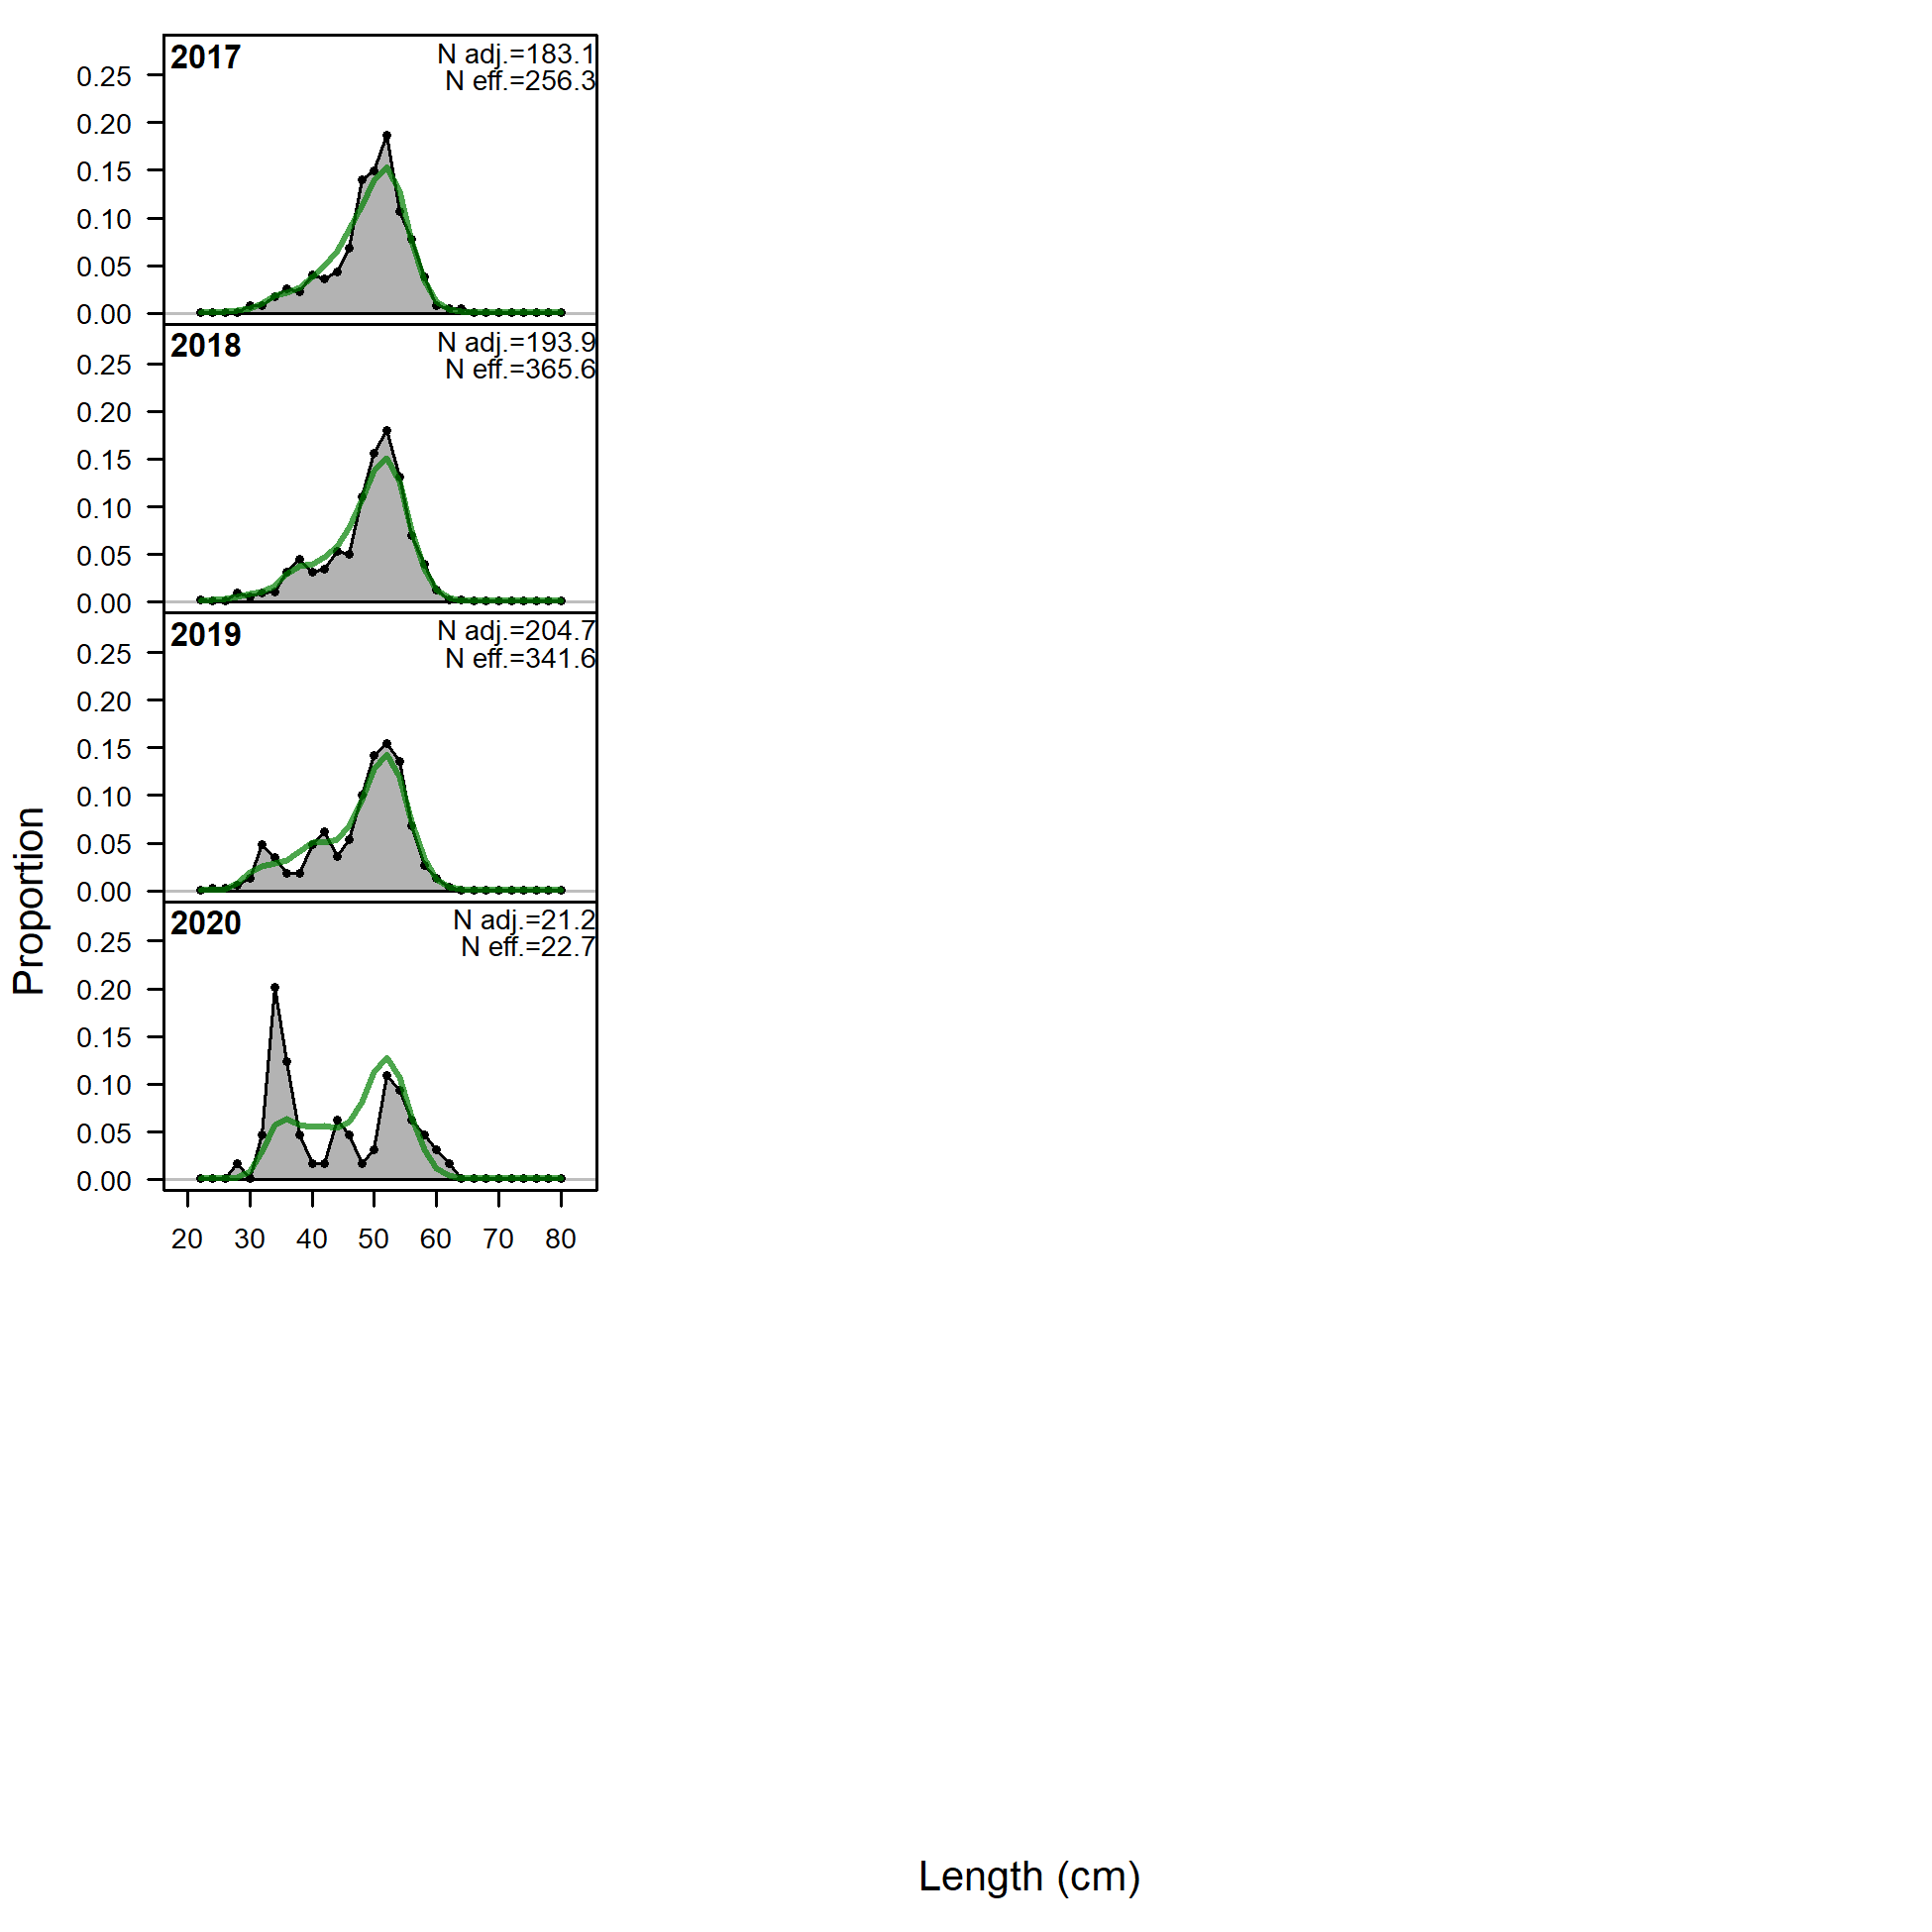
\includegraphics[width=1\textwidth,height=1\textheight]{C:/Users/Jason.Cope/Documents/Github/Vermilion rockfish OR WA assessment 2021/OR/write_up/models/Reference model/plots/comp_lenfit_flt2mkt0_page2.png}
\caption{Length comps, whole catch, Recreational (plot 2 of 2).\label{fig:comp_lenfit_flt2mkt0_page2}}
\end{figure}

\tagmcend\tagstructend

\tagstructbegin{tag=H1}\tagmcbegin{tag=H1}

\hypertarget{detailed-fit-to-conditional-age-at-length-composition-data}{%
\section{Detailed Fit to Conditional-Age-at-Length Composition Data}\label{detailed-fit-to-conditional-age-at-length-composition-data}}

\leavevmode\tagmcend\tagstructend

\tagstructbegin{tag=Figure,alttext={Pearson residuals, whole catch, Commercial (max=30.56) (plot 1 of 4) (plot 2 of 4).}}\tagmcbegin{tag=Figure}

\begin{figure}
\centering
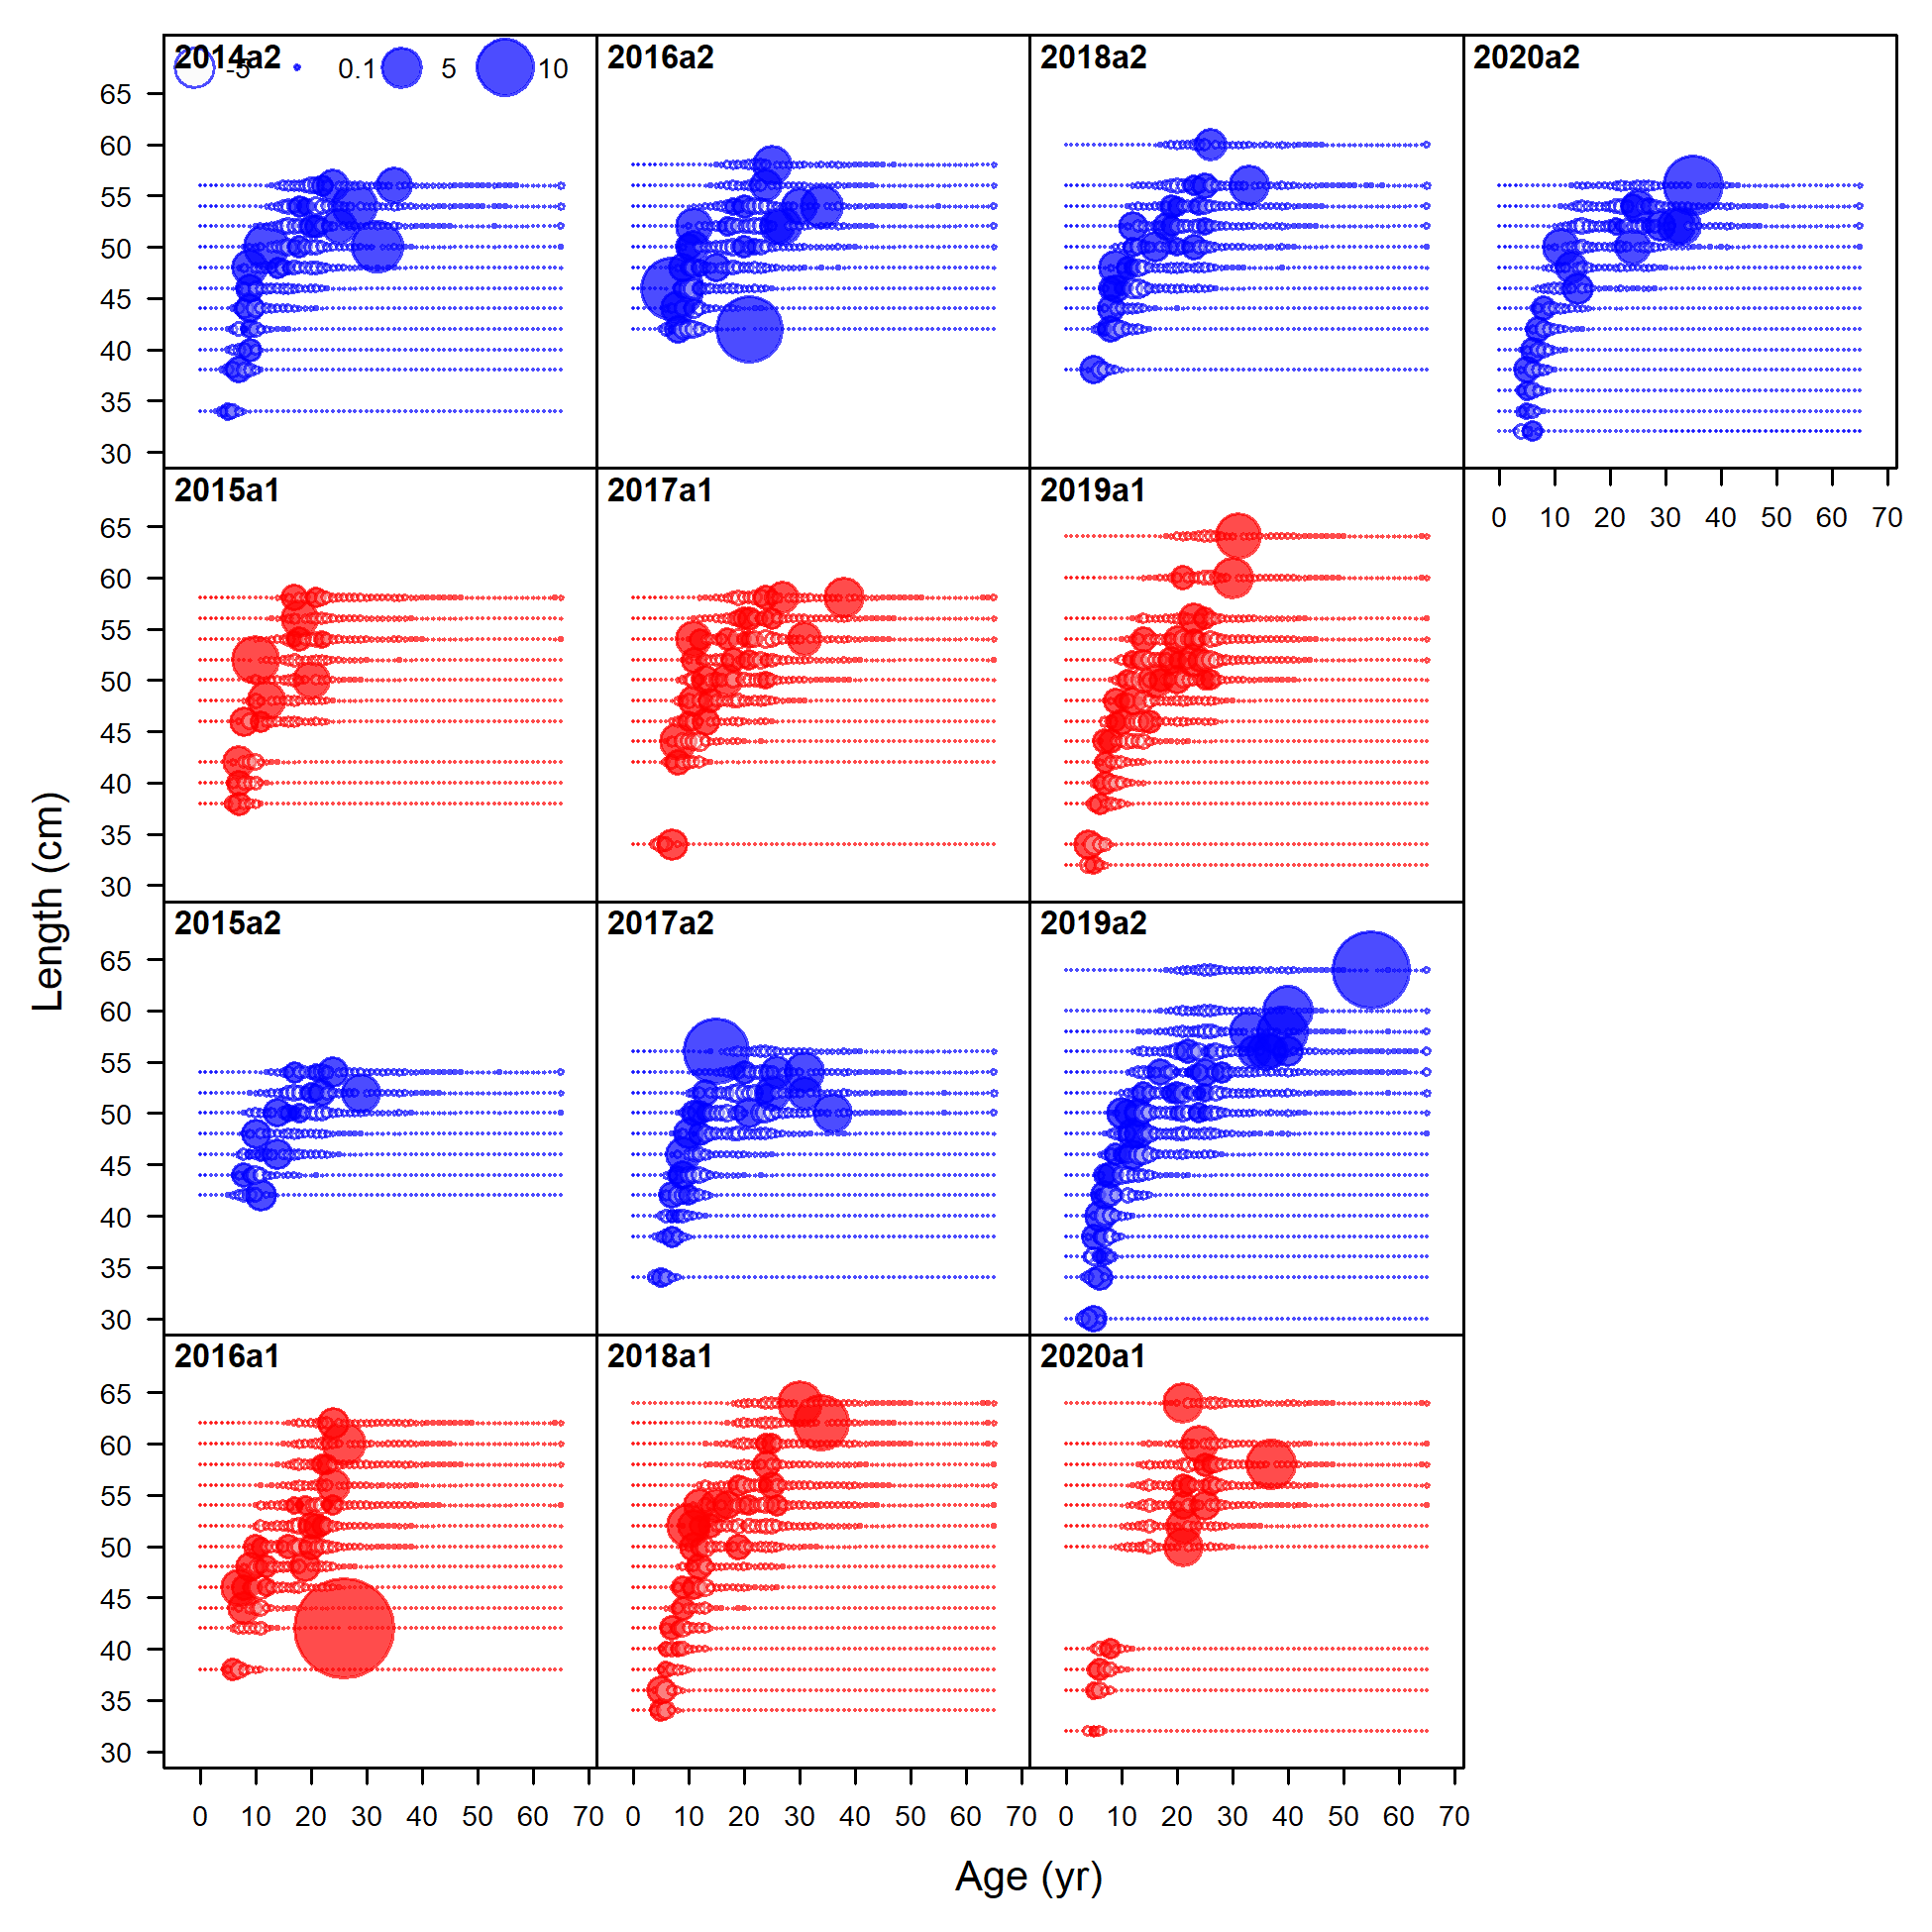
\includegraphics[width=1\textwidth,height=1\textheight]{C:/Users/Jason.Cope/Documents/Github/Vermilion rockfish OR WA assessment 2021/OR/write_up/models/Reference model/plots/comp_condAALfit_residsflt1mkt0_page2.png}
\caption{Pearson residuals, whole catch, Commercial (max=30.56) (plot 1 of 4) (plot 2 of 4).\label{fig:comp_condAALfit_residsflt1mkt0_page2}}
\end{figure}

\tagmcend\tagstructend

\tagstructbegin{tag=Figure,alttext={Pearson residuals, whole catch, Commercial (max=30.56) (plot 1 of 4) (plot 2 of 4) (plot 3 of 4).}}\tagmcbegin{tag=Figure}

\begin{figure}
\centering

\includegraphics[width=1\textwidth,height=1\textheight]{C:/Users/Jason.Cope/Documents/Github/Vermilion rockfish OR WA assessment 2021/OR/write_up/models/Reference model/plots/comp_condAALfit_residsflt1mkt0_page3.png}
\caption{Pearson residuals, whole catch, Commercial (max=30.56) (plot 1 of 4) (plot 2 of 4) (plot 3 of 4).\label{fig:comp_condAALfit_residsflt1mkt0_page3}}
\end{figure}

\tagmcend\tagstructend

\tagstructbegin{tag=Figure,alttext={Pearson residuals, whole catch, Commercial (max=30.56) (plot 1 of 4) (plot 2 of 4) (plot 3 of 4) (plot 4 of 4).}}\tagmcbegin{tag=Figure}

\begin{figure}
\centering

\includegraphics[width=1\textwidth,height=1\textheight]{C:/Users/Jason.Cope/Documents/Github/Vermilion rockfish OR WA assessment 2021/OR/write_up/models/Reference model/plots/comp_condAALfit_residsflt1mkt0_page4.png}
\caption{Pearson residuals, whole catch, Commercial (max=30.56) (plot 1 of 4) (plot 2 of 4) (plot 3 of 4) (plot 4 of 4).\label{fig:comp_condAALfit_residsflt1mkt0_page4}}
\end{figure}

\tagmcend\tagstructend

\tagstructbegin{tag=Figure,alttext={Pearson residuals, whole catch, Recreational (max=30.63) (plot 1 of 3).}}\tagmcbegin{tag=Figure}

\begin{figure}
\centering
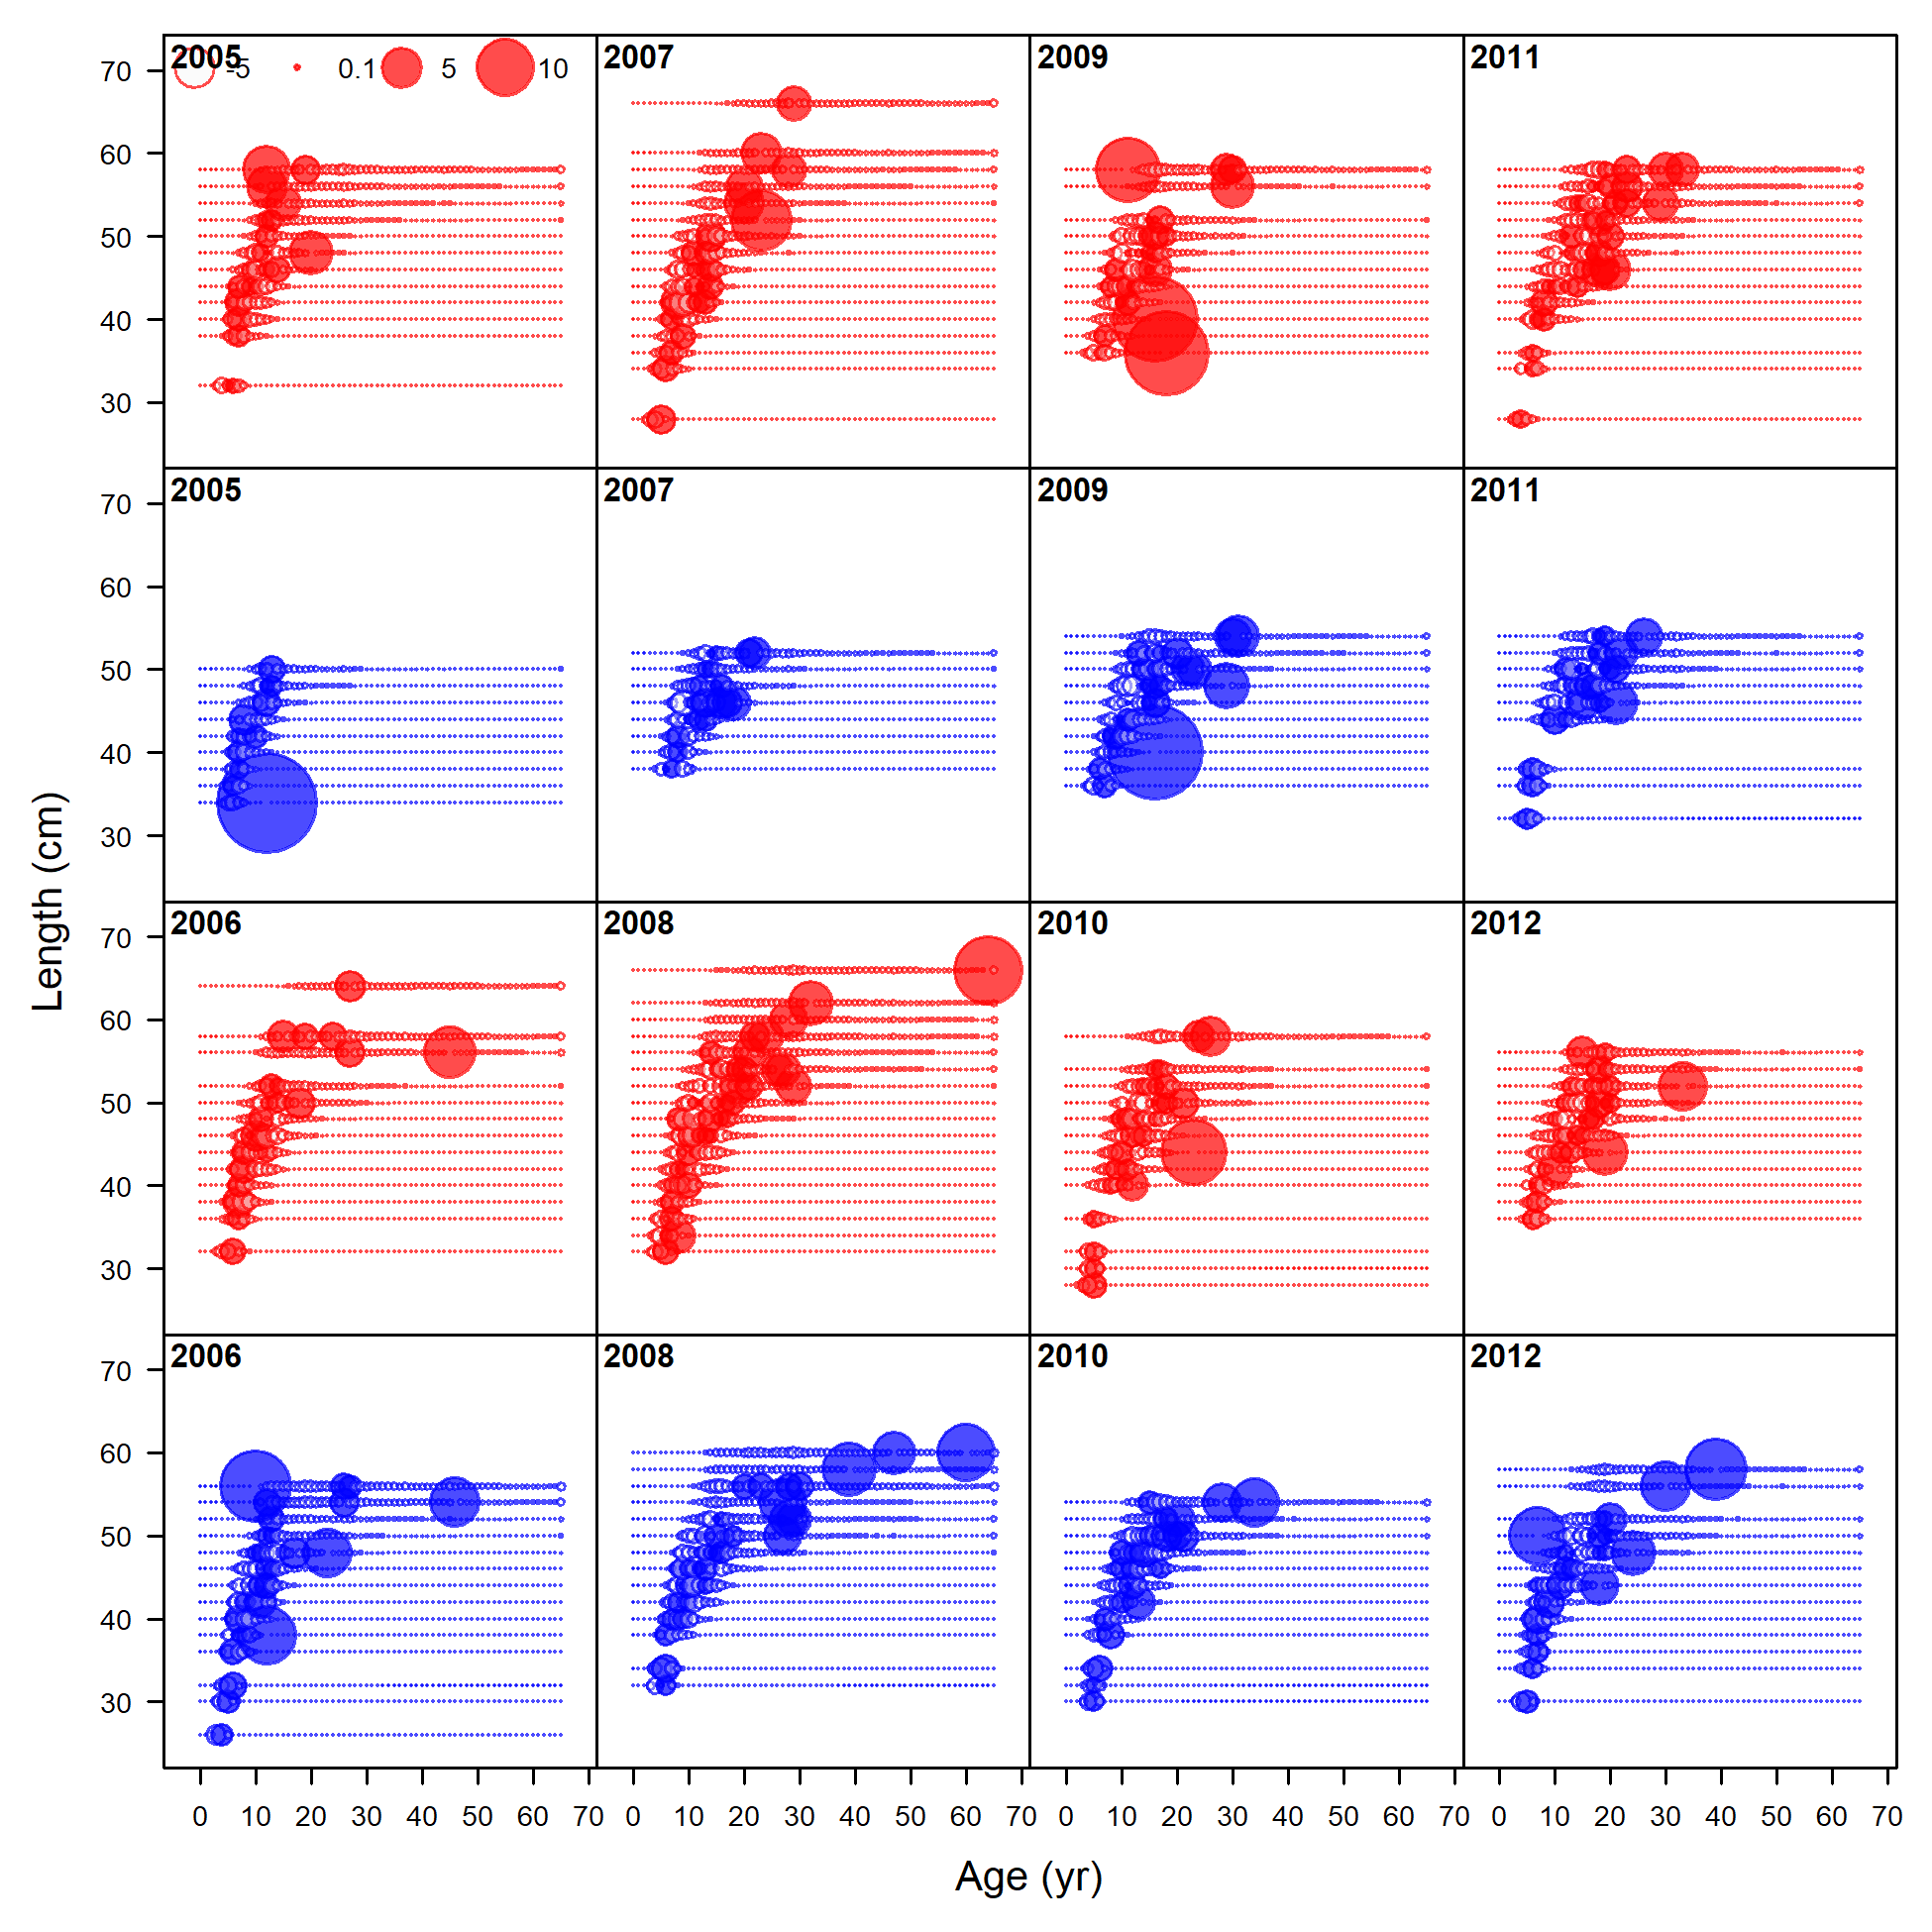
\includegraphics[width=1\textwidth,height=1\textheight]{C:/Users/Jason.Cope/Documents/Github/Vermilion rockfish OR WA assessment 2021/OR/write_up/models/Reference model/plots/comp_condAALfit_residsflt2mkt0_page1.png}
\caption{Pearson residuals, whole catch, Recreational (max=30.63) (plot 1 of 3).\label{fig:comp_condAALfit_residsflt2mkt0_page1}}
\end{figure}

\tagmcend\tagstructend

\tagstructbegin{tag=Figure,alttext={Pearson residuals, whole catch, Recreational (max=30.63) (plot 1 of 3) (plot 2 of 3).}}\tagmcbegin{tag=Figure}

\begin{figure}
\centering
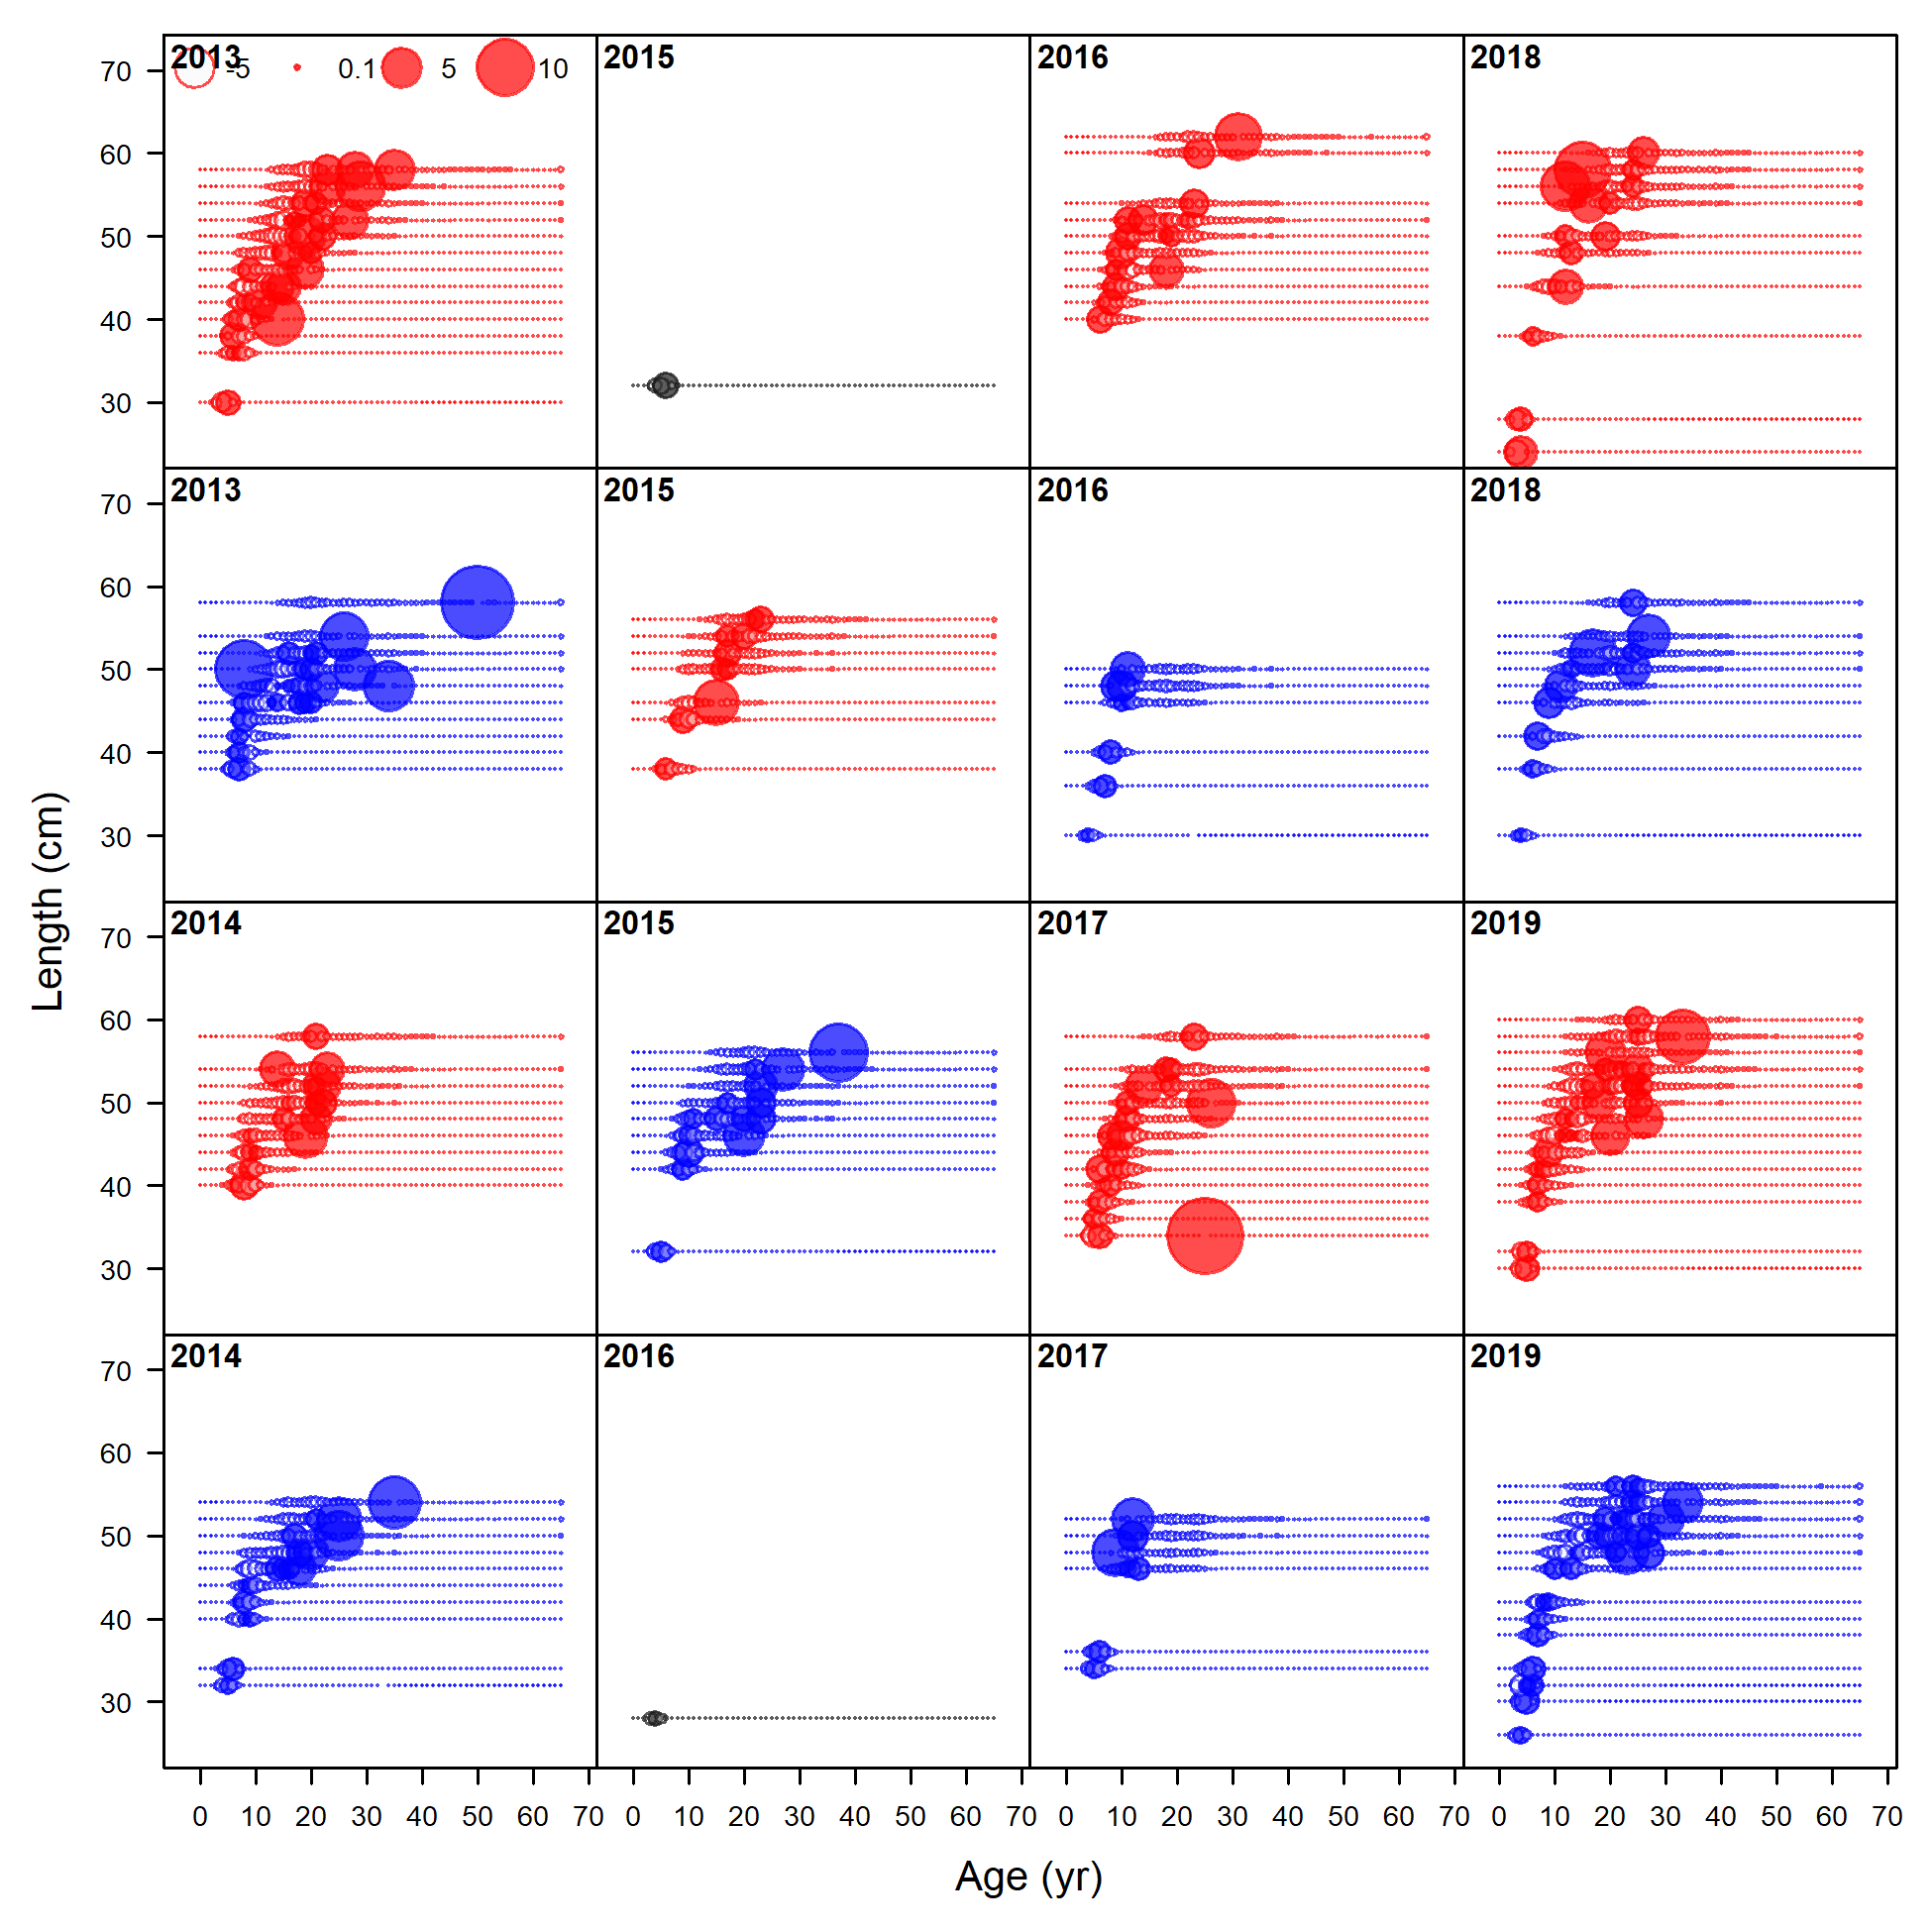
\includegraphics[width=1\textwidth,height=1\textheight]{C:/Users/Jason.Cope/Documents/Github/Vermilion rockfish OR WA assessment 2021/OR/write_up/models/Reference model/plots/comp_condAALfit_residsflt2mkt0_page2.png}
\caption{Pearson residuals, whole catch, Recreational (max=30.63) (plot 1 of 3) (plot 2 of 3).\label{fig:comp_condAALfit_residsflt2mkt0_page2}}
\end{figure}

\tagmcend\tagstructend

\tagstructbegin{tag=Figure,alttext={Pearson residuals, whole catch, Recreational (max=30.63) (plot 1 of 3) (plot 2 of 3) (plot 3 of 3).}}\tagmcbegin{tag=Figure}

\begin{figure}
\centering
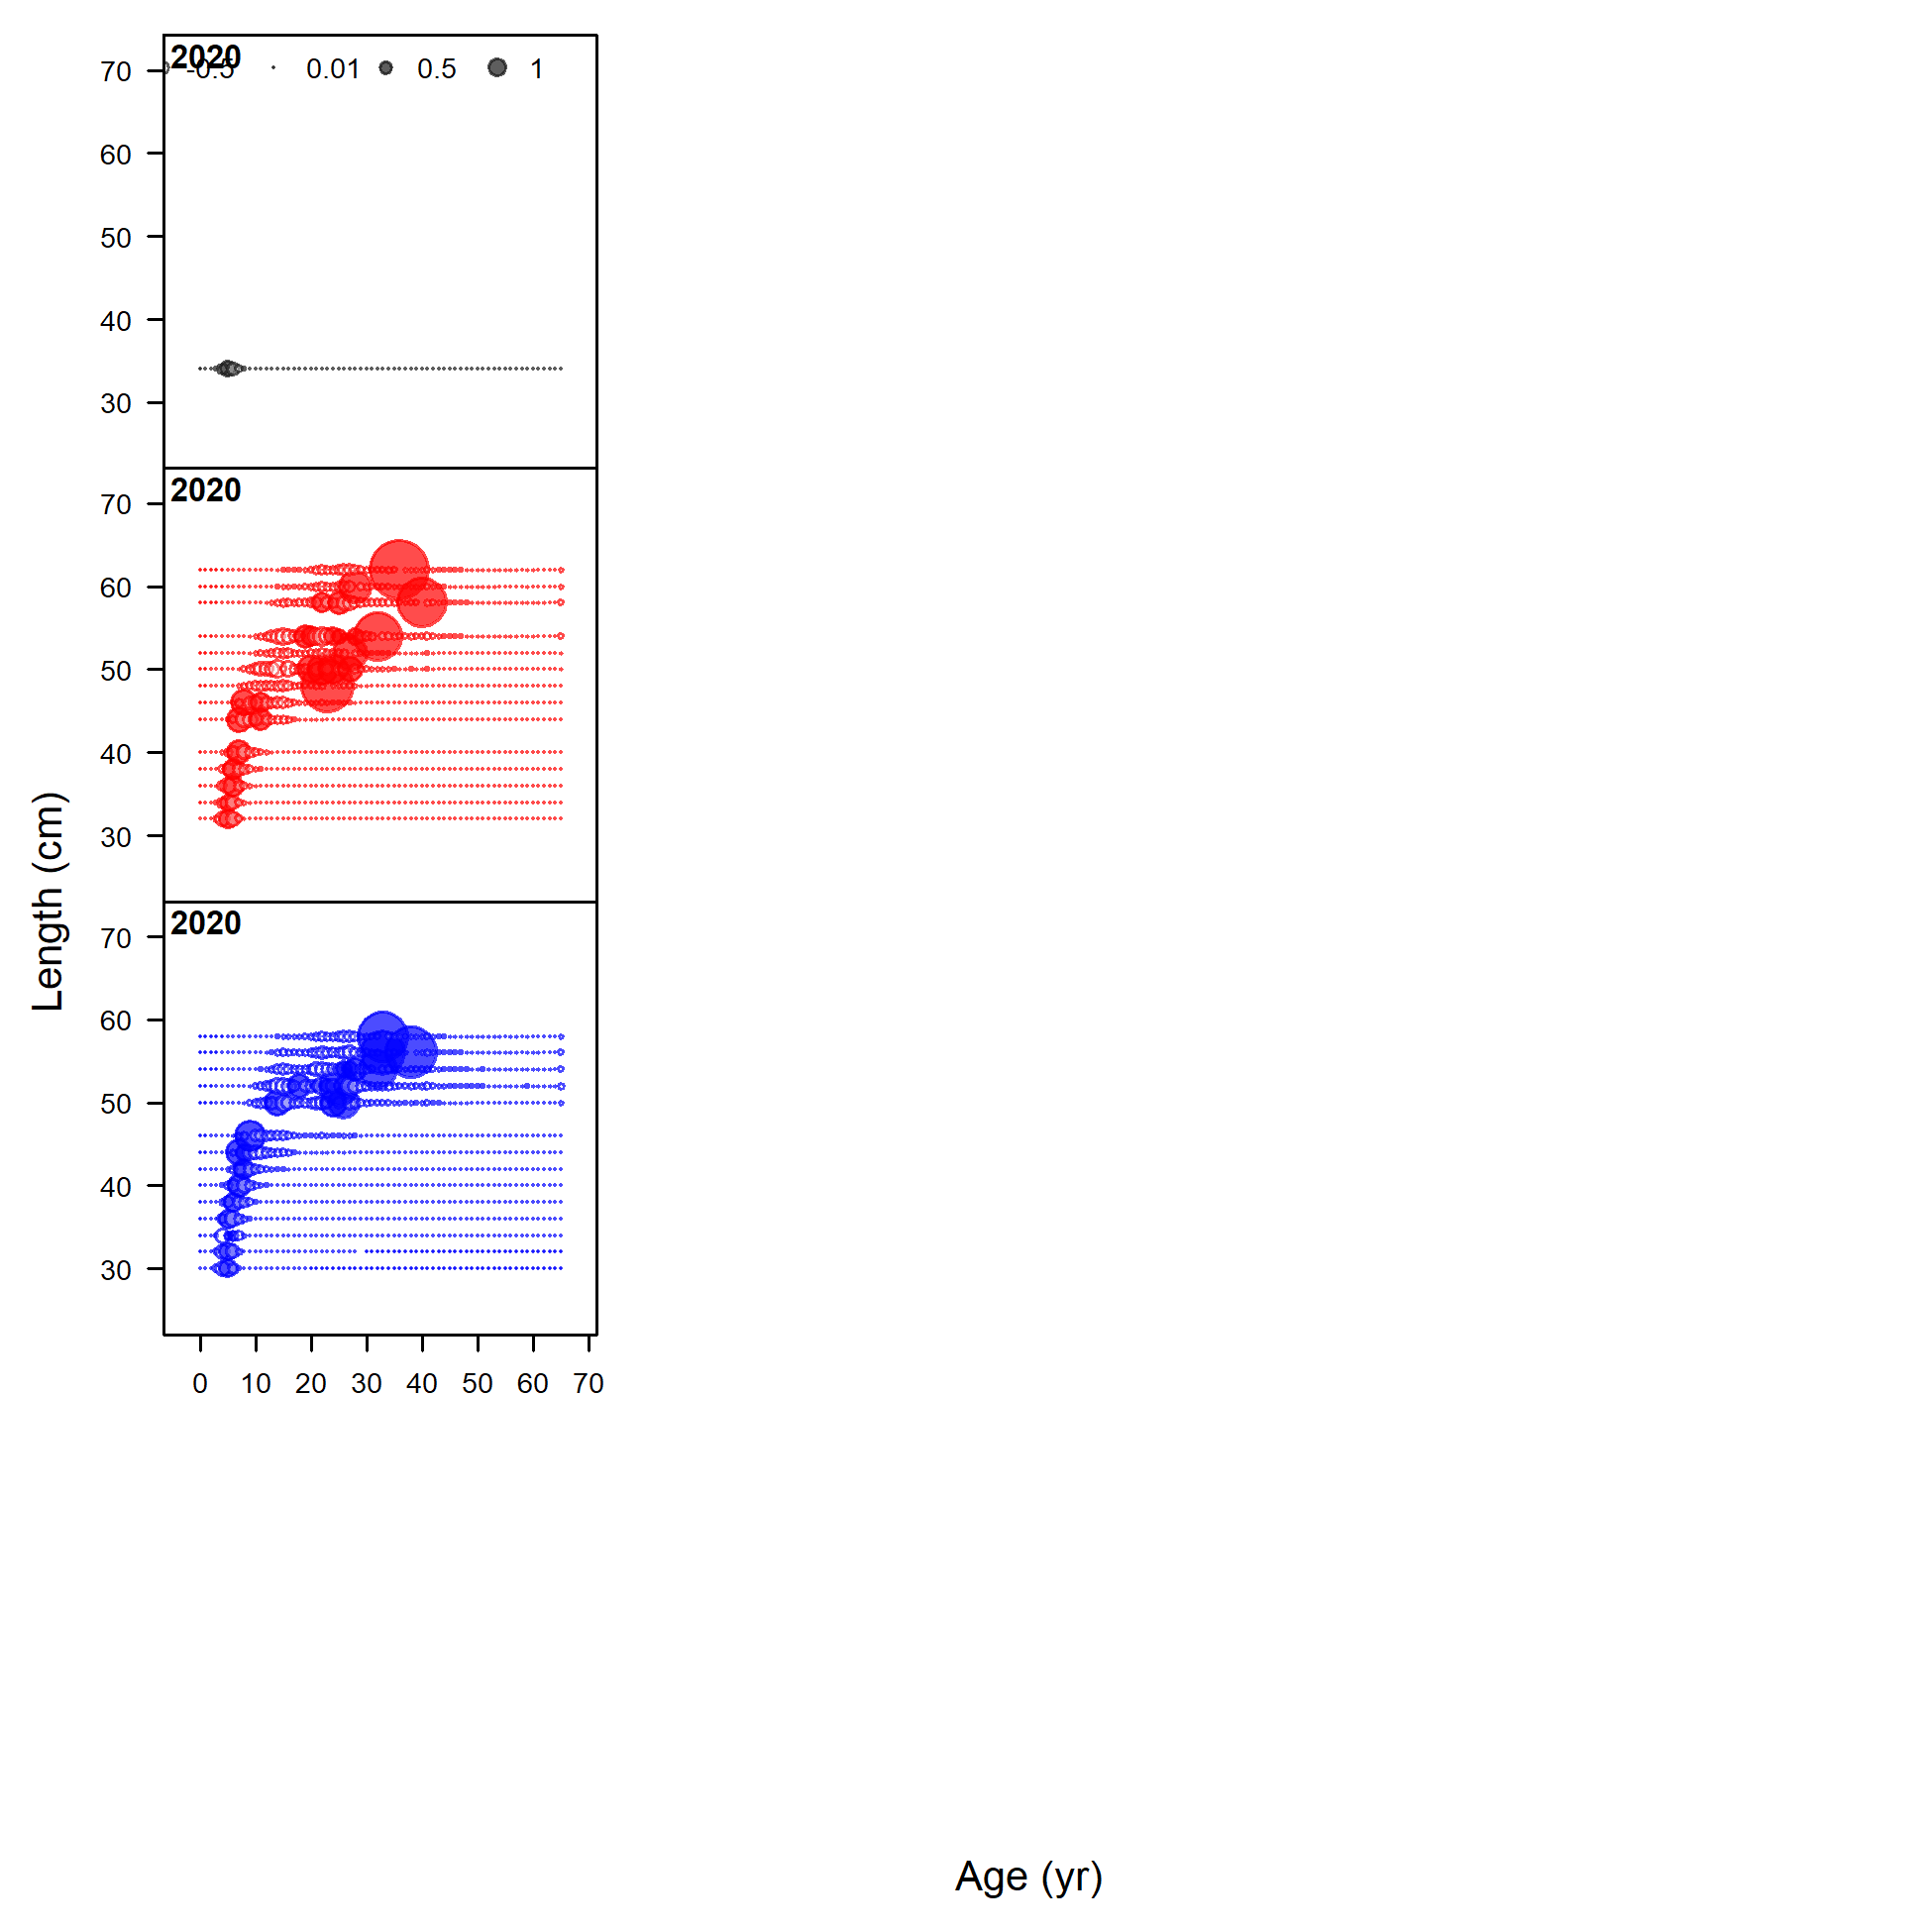
\includegraphics[width=1\textwidth,height=1\textheight]{C:/Users/Jason.Cope/Documents/Github/Vermilion rockfish OR WA assessment 2021/OR/write_up/models/Reference model/plots/comp_condAALfit_residsflt2mkt0_page3.png}
\caption{Pearson residuals, whole catch, Recreational (max=30.63) (plot 1 of 3) (plot 2 of 3) (plot 3 of 3).\label{fig:comp_condAALfit_residsflt2mkt0_page3}}
\end{figure}

\tagmcend\tagstructend
\end{document}
